\documentclass[12pt,a4paper]{book}
\usepackage[utf8]{inputenc}
%\usepackage{amsmath}
\usepackage{mathtools}
\usepackage{amsfonts}
\usepackage{amssymb}
\usepackage{listings}
\usepackage{url}
\usepackage[bulgarian]{babel}
\usepackage{listings}
\usepackage{enumerate}
\usepackage[framemethod=tikz]{mdframed}
\usepackage{enumitem}
\usepackage{relsize}
\usepackage{hyperref}
\usepackage{caption}
\usepackage{tikz}
\usetikzlibrary{shapes,arrows,positioning,calc,positioning,fit,chains}
\usepackage{forest}


\captionsetup{font=footnotesize}

\lstset{breaklines=true}

\setenumerate[1]{label=\thesection.\arabic*.}
\setenumerate[2]{label*=\arabic*.}

\newcommand{\code}[1]{\texttt{#1}}

\hypersetup{
    colorlinks,
    citecolor=black,
    filecolor=black,
    linkcolor=black,
    urlcolor=black
}

\tikzset{
block/.style = {draw, fill=white, rectangle,align = center},
entry/.style = {draw, fill=black, circle, radius=3em},
condition/.style = {draw, fill=white, diamond, align = center,node distance=3cm},
fork/.style = {draw, fill=black, circle,inner sep=1pt},
}
\tikzset{
block/.style = {draw, fill=white, rectangle,align = center},
entry/.style = {draw, fill=black, circle, radius=3em},
condition/.style = {draw, fill=white, diamond, align = center,node distance=3cm},
fork/.style = {draw, fill=black, circle,inner sep=1pt},
lnode/.style={rectangle split, rectangle split parts=3,draw, rectangle split horizontal},
treenode/.style = {align=center, inner sep=0pt, text centered, circle, font=\sffamily\bfseries, draw=black, fill=white, text width=1.5em}
}

\renewcommand{\thesection}{\arabic{section}}
\raggedbottom 

\author{\textit{Калин Георгиев}\\
\small{kalin@fmi.uni-sofia.bg}}
\title{\textsc{Задачи за задължителна самоподготовка} \\
по \\
Увод в програмирането, Обектно-ориентирано програмиране и Структури от данни}


\begin{document}
\maketitle

\tableofcontents

\pagebreak

\small{Някои от задачите по-долу са решени в сборника \cite{sbornik}\textit{Магдалина Тодорова, Петър Армянов, Дафина Петкова, Калин Георгиев, ``Сборник от задачи по програмиране на C++. Първа част. Увод в програмирането''}. За задачите от сборника е посочена номерацията им от сборника.}

\pagebreak

\chapter{Увод в програмирането}
\section {Увод, основи и примери}

\subsection {Основни примери}

\begin{enumerate}

	\item Превърнете рождената си дата шестнадесетична, в осмична и в двоична бройни системи.

	\item Как бихте кодирали вашето име само с числа? Измислете собствено представяне на символни константи чрез редици от числа и запишете името си в това представяне.

	Разгледайте стандартната ASCii таблица (\code{http://www.asciitable.com/}) и запишете името си чрез серия от ASCii кодове.

\end{enumerate}

\subsection {Променливи, вход и изход, логически и аритметични операции, условен оператор}

\begin{enumerate}[resume]

	\item Задача 1.6.\cite{sbornik} Да се напише програма, която по зададени навършени години намира приблизително броя на дните, часовете, минутите и секундите, които е живял човек до навършване на зададените години.

	\item Задача 1.7.\cite{sbornik} Да се напише програма, която намира лицето на триъгълник по дадени: а) дължини на страна и височина към нея; б) три страни.


	\item Задача 2.7.\cite{sbornik} Да се напише програма, която въвежда координатите на точка от равнина и извежда на кой квадрант принадлежи тя. Да се разгледат случаите, когато точката принадлежи на някоя от координатните оси или съвпада с центъра на координатната система.

	\item Задача 1.14.\cite{sbornik} Да се запише булев израз, който да има стойност истина, ако посоченото условие е вярно и стойност - лъжа, в противен случай:

	\renewcommand{\theenumii}{\Alph{enumii}}

	\begin{enumerate}[label=\alph*)]%[a)] % a), b), c), ...
			 \item цялото число p се дели на 4 или на 7;
			 \item уравнението $ax^2 + bx + c = 0 (a \neq 0)$ няма реални корени;
			 \item точка с координати (a, b) лежи във вътрешността на кръг с радиус 5 и център (0, 1); г) точка с координати (a, b) лежи извън кръга с център (c, d) и радиус f;
			 \item точка принадлежи на частта от кръга с център (0, 0) и радиус 5 в трети квадрант;
			 \item точка принадлежи на венеца с център (0, 0) и радиуси 5 и 10;
			 \item x принадлежи на отсечката [0, 1];
			 \item x е равно на max \{a, b, c\};
			 \item x е различно от max \{ a, b, c\};
			 \item поне една от булевите променливи x и y има стойност true;
			 \item и двете булеви променливи x и y имат стойност true;
			 \item нито едно от числата a, b и c не е положително;
			 \item цифрата 7 влиза в записа на положителното трицифрено число p;
			 \item цифрите на трицифреното число m са различни;
			 \item поне две от цифрите на трицифреното число m са равни помежду си;
			 \item цифрите на трицифреното естествено число x образуват строго растяща или строго намаляваща редица;
			 \item десетичните записи на трицифрените естествени числа x и y са симетрични;
			 \item естественото число x, за което се знае, че е по-малко от 23, е просто.
  \end{enumerate}


\item Задача 2.12.\cite{sbornik} Да се напише програма, която проверява дали дадена година е високосна.

\end{enumerate}

\subsection {Цикли}

\begin{enumerate}[resume]


	\item Задача 1.20.\cite{sbornik} Да се напише програма, която по въведени от клавиатурата цели числа x и k ($k \geq 1$) намира и извежда на екрана k-тата цифра на х. Броенето да е отдясно наляво.

	\item Задача 2.40.\cite{sbornik} Да се напише програма, която (чрез цикъл for) намира сумата на всяко трето цяло число, започвайки от 2 и ненадминавайки n (т.е. сумата 2 + 5 + 8 + 11 + ...).

	\item Задача 2.44.\cite{sbornik} Дадено е естествено число n ($n \geq 1$). Да се напише програма, която намира броя на тези елементи от серията числа $i^3 + 13 \times i \times n + n
	^3$ , $i = 1, 2, ..., n$, които са кратни на 5 или на 9.

	\item За въведени от клавиатурата естествени числа $n$ и $k$, да се провери и изпише на екрана дали $n$ е точна степен на числото $k$.

	\textit{Упътване: Разделете променливата $n$ на променливата $k$ ``колкото пъти е възможно'' и проверете дали $n$ достига единица или някое друго число след края на процеса. Използвайте добре подбрано условие за for цикъл, оператора \% за намиране на остатък при целочислено деление, и оператора за целочислено деление /.}

\end{enumerate}


\subsection {Машини с неограничени регистри}


\small{Дефиницията на Машина с неограничени регистри по-долу е взаимствана от учебника \cite{tprog}\textit{А. Дичев, И. Сосков, ``Теория на програмите'', Издателство на СУ, София, 1998}.

\vspace{20px}

\begin{mdframed}[hidealllines=true,backgroundcolor=gray!20]

	``Машина с неограничени регистри'' (или МНР) наричаме абстрактна машина, разполагаща с неограничена памет. Паметта на машината се представя с безкрайна редица от естествени числа $m[0],m[1],...$, където $m[i] \in \mathcal{N}$. Елементите $m[i]$ на редицата наричаме ``клетки'' на паметта на машината, а числото $i$ наричаме ``адрес'' на клетката $m[i]$.

	 МНР разполага с набор от инструкции за работа с паметта. Всяка инструкция получава един или повече параметри (операнди) и може да предизвика промяна в стойността на някоя от клетките на паметта. Инструкциите на МНР за работа с паметта са:

	\begin{enumerate}[label=\arabic*)]
		\item \code{ZERO n}: Записва стойността 0 в клетката с адрес $n$
		\item \code{INC n}: Увеличава с единица стойността, записана в клетката с адрес $n$
		\item \code{MOVE x y}: Присвоява на клетката с адрес $y$ стойността на клетката с адрес $x$
	\end{enumerate}

	``Програма'' за МНР наричаме всяка последователност от инструкции на МНР и съответните им операнди. Всяка инструкция от програмата индексираме с поредния ѝ номер. Изпълнението на програмата започва от първата инструкция и преминава през всички инструкции последователно, освен в някои случаи, описани по-долу. Изпълнението на програмата се прекратява след изпълнението на последната ѝ инструкция. Например, след изпълнението на следната програма:

	\begin{verbatim}
	0: ZERO 0
	1: ZERO 1
	2: ZERO 2
	3: INC 1
	4: INC 2
	5: INC 2
	\end{verbatim}

	Първите три клетки на машината ще имат стойност 0, 1, 2, независимо от началните им стойности.

	Освен инструкциите за работа с паметта, МНР притежават и една инструкция за промяна на последователността на изпълнение на програмата:

	\begin{enumerate}[label=\arabic*)]
	\setcounter{enumi}{3}
		\item \code{JUMP x}: Изпълнението на програмата ``прескача'' и продължава от инструкцията с пореден номер $x$. Ако програмата има по-малко от $x+1$ инструкции, изпълнението ѝ се прекратява
		\item \code{JUMP x y z}: Ако съдържанията на клетките  $x$ и $y$ съвпадат, изпълнението на програмата ``прескача'' и продължава от инструкцията с пореден номер $z$. В противен случай, програмата продължава със следващата инструкция. Ако програмата има по-малко от $z+1$ инструкции, изпълнението ѝ се прекратява
	\end{enumerate}

	Например, нека изпълнението на следната програма започва при стойности на клетките на паметта 10,0,0,...:

	\begin{verbatim}
	0: JUMP 0 1 5
	1: INC 1
	2: INC 2
	3: INC 2
	4: JUMP 0
	\end{verbatim}

	След приключване на програмата, първите три клетки на машината ще имат стойности 10, 10, 20.

\end{mdframed}

\begin{enumerate}[resume]
	\item Нека паметта на МНР е инициализирана с редицата $m,n,0,0,...$. Да се напише програма на МНР, след изпълнението на която клетката с адрес 2 съдържа числото $m+n$.
	\item Нека паметта на МНР е инициализирана с редицата $m,n,0,0,...$. Да се напише програма на МНР, след изпълнението на която клетката с адрес 2 съдържа числото $m \times n$.
	\item Нека паметта на МНР е инициализирана с редицата $m,n,0,0,...$. Да се напише програма на МНР, след изпълнението на която клетката с адрес 2 съдържа числото 1 тогава и само тогава, когато $m>n$ и числото 0 във всички останали случаи.
\end{enumerate}

\begin{mdframed}[hidealllines=true,backgroundcolor=gray!20]
\textbf{Упътване:} На Фигура \ref{fig:mnr}~(a) е показана блок схема на програма, използваща само операторите \code{=}, \code{==}, \code{++} и \code{if}, която намира в променливата \code{result} сумата на променливите $a_0$ и $a_1$. $a_0$ и $a_1$ считаме за дадени. Променливата \code{count} се инициализира с 0, а \code{result} - с $a_0$. В цикъл се добавя по една единица към \code {count} и \code{result} дотогава, докато \code{count} достигне стойността на $a_1$. По този начин, към \code{result} се добавят $a_1$ на брой единици, т.е. стойността ѝ се увеличава с $a_1$ спрямо началната ѝ стойност $a_0$.

На Фигура \ref{fig:mnr}~(b) е показана същата програма, като операторите от първата са заменени със съответните им инструкции на МНР. Резултатът от програмата се получава в клетката $m[2]$, а за брояч се ползва клетката $m[3]$. На блок схемата са дадени поредните номера на инструкциите в окончателната програмата на МНР:
\begin{verbatim}
0:MOVE 0 2
1:ZERO 3
2:JUMP 1 3 6
3:INC 2
4:INC 3
5:JUMP 2
\end{verbatim}
\end{mdframed}

\begin{figure}
\relscale{0.7}
  \begin{tabular}{p{7cm} p{7cm}}
      \begin{tikzpicture}[auto, node distance=1.5cm,>=latex']
      \node [entry, name=start](start){};
      \node [block,name=init, below of = start] (init)
         {\code{result:=$a_0$}\\\code{counter:=0}};
      \node [fork,name=test1fork,below of = init,node distance = 1cm]{};
      \node [condition,name=test1, below of = test1fork,node distance = 2cm] (test1) {\code{counter==$a_1$}};
      \node [block,name=inc,right of = test1, node distance = 3cm] (inc) {\code{$a_0$++}\\\code{counter++}};
      \node [entry, name=end, below of = test1, node distance = 2.5cm](end){};
      \draw [->] (start) -- (init);
      \draw [-] (init) -- (test1fork);
      \draw [->] (test1fork) -- (test1);
      \draw [->] (test1) -- node{no} (inc);
      \draw [->] (inc) |- (test1fork);
      \draw [->] (test1) -- node []{yes}(end);
      \end{tikzpicture}

      &

      \begin{tikzpicture}[auto, node distance=1.5cm,>=latex']
      \node [entry, name=start](start){};
      \node [block,name=init, below of = start, align = left] (init)
         {\code{0:MOVE 0 2}\\\code{1:ZERO 3}};
      \node [fork,name=test1fork,below of = init,node distance = 1cm]{};
      \node [condition,name=test1, below of = test1fork,node distance = 2cm] (test1) {\code{2:JUMP 1 3 6}};
      \node [block,name=inc,right of = test1, node distance = 3cm,align = left] (inc) {\code{3:INC 2}\\\code{4:INC 3}\\\code{5:JUMP 3}};
      \node [entry, name=end, below of = test1, node distance = 2.5cm](end){};
      \draw [->] (start) -- (init);
      \draw [-] (init) -- (test1fork);
      \draw [->] (test1fork) -- (test1);
      \draw [->] (test1) -- node{} (inc);
      \draw [->] (inc) |- (test1fork);
      \draw [->] (test1) -- node []{}(end);
      \end{tikzpicture}

      \\
      (a)Програма за сумиране на числата $a_0$ и $a_1$ с изпозлване само на операторите \code{=}, \code{==}, \code{++} и \code{if}.
      &
      (b)Програма за сумиране на клетките $m[0]$ и $m[1]$ с инструкции на МНР.
  \end{tabular}

  \caption{Блок схеми на програма за сумиране на числа}
  \label{fig:mnr}
\end{figure}




\pagebreak

\clearpage\section {Типове и функции}

\subsection {Прости примери за функции}

\begin{enumerate}[]
	\item Задача 4.12.\cite{sbornik} Да се напише булева функция, която проверява дали дата, зададена в следния формат: dd.mm.yyyy е коректна дата от грегорианския календар.
	\item Задача 4.25.\cite{sbornik} Да се дефинира процедура, която получава целочислен параметър $n$ и база на бройна система $k \leq 16$. Процедурата да отпечатва на екрана представянето на числото $n$ в системата с база $k$.
	\item Задача 2.57.\cite{sbornik}	Да се напише булева функция, която проверява дали сумата от цифрите на дадено като параметър положително цяло число е кратна на 3.
	\item Задача 2.81.\cite{sbornik} Едно положително цяло число е съвършено, ако е равно на сумата от своите делители (без самото число). Например, 6 е съвършено, защото 6 = 1+2+3; числото 1 не е съвършено. Да се напише процедура, която намира и отпечатва на екрана  всички съвършени числа, ненадминаващи дадено положително цяло число в параметър n.

\end{enumerate}

\subsection {Елементарна растерна графика}

  \begin{mdframed}[hidealllines=true,backgroundcolor=gray!20]

  Следните задачи да се решат с показаните на лекции графични примитиви, базирани на платформата за компютърни игри SDL2. За целта е необходимо да инсталирате SDL2 на компютъра си и да настроите средата си за програмиране така, че да свърже SLD2 с вашия проект. Информация за това можете да намерите на сайта на платформата.
	Задачите можете да решите с помощта на всяка друга библиотека, поддържаща примитивите за рисуване на точки и отсечки.

  Примерната програма от лекции използва модула \code{Sdlwrapper}, който можете да намерите в \href{https://github.com/stranxter/lecture-notes/tree/master/samples/01_programming%20101/2022-23-kn/pixels/draw}{\underline{хранилището на курса}}:
  \begin{mdframed}[hidealllines=true,backgroundcolor=lightgray!20]
  \relscale{0.8}
  \begin{verbatim}
  #include "draw/sdlwrapper.h"
  \end{verbatim}
  \end{mdframed}

  \code{Sdlwrapper} ``обвива'' библиотеката SLD2 и дефинира следните лесни за използване примитиви:

  \begin{itemize}
    \item \code{setColor (r,g,b)}: Дефинира цвят на рисуване с компоненти $r,g,b\in[0,255]$. Например, белият цвят се задава с $(255,255,255)$, червеният с $(255,0,0)$ и т.н.
    \item \code{drawPixel(x,y)}: Поставя една точка на екранни координати $(x,y)$.
    \item \code{drawLine (x1,y1,x2,y2)}: Рисува отсечка, свързваща точките с екранни координати $(x_1,y_1)$ и $(x_2,y_2)$.
    \item \code{updateGraphics()}: Извиква се веднъж в края на програмата, за да се изобрази нарисуваното с горните примитиви.
  \end{itemize}
\end{mdframed}

\begin{figure}
  \begin{center}
  \relscale{0.7}
  \begin{tabular}{|p{5.2cm}p{5.2cm}|}
   \hline
   \vspace{10pt}
   \includegraphics[width=3cm]{images/graph_sine} &
   \vspace{10pt}
   \includegraphics[width=3cm]{images/graph_sine_coarse}\\
   (a)Графика на $y=sin(x)$, нарисувана с 300 отсечки&
   (b)Графика на $y=sin(x)$ с 10 отсечки. Нарисувани са също отсечки между точките от графиката на функцията и абсцисата\\%\hline
   \vspace{10pt}
   \includegraphics[width=3cm]{images/graph_4_polygons}  &
   \vspace{10pt}
   \includegraphics[width=3cm]{images/graph_16_polygons}  \\
   (c)Четири многоъгълника, нарисувани един върху друг с нарастващи радиус и брой върхове
   \vspace{10pt}&
   (d)Шестнадесет многоъгълника, нарисувани един върху друг с нарастващи радиус и брой върхове
   \vspace{10pt}  \\%\hline
   \vspace{10pt}
   \includegraphics[width=3cm]{images/graph_twentygon}   &
    \\
    (e)Многоъгълник с 20 върха, приближаващ окръжност
   \vspace{10pt} &
   \\\hline
  \end{tabular}
  \end{center}

  \caption{Примерни резултати от решенията на някои задачи}
  \label{fig:drawings}
\end{figure}



\begin{enumerate}[resume]


	\item Да се нарисуват програмно следните фигури чрез дефиниране на подходящи функции:

	\begin{itemize}
		\item Равностранен триъгълник по дадена дължина на страната
		\item Равностранен шестоъгълник по дадена дължина на страната
		\item Графиката на функциите $y=sin(x)$, $y=x^2$, и $y=x^3+5x^2$ поотделно и заедно
    \item Равностранен многоъгълник по дадени координати на пресечната точка на симетралите му (център), брой страни $n$ и разстояние от центъра до върховете $r$. При какви стойности на $n$ фигурата наподобява окръжност?
		\item Логаритмична крива
		\item Елипса с център дадени $(x,y)$ и радиуси дадени $r_1$ и $r_2$
	\end{itemize}

	\item По дадени екранни координати $(x,y)$ на горния ляв ъгъл на квадрат, дължина на страната $a$ на квадрата и число $n$:

	\begin{itemize}
		\item Да се нарисува квадратна матрица от $n \times $n квадрата със страна $a/n$, изпълваща дадения квадрат.
		\item Квадратите от горното условие да се заменят с триъгълниците, образувани от пресичането на диагоналите им.
	\end{itemize}




\begin{mdframed}[hidealllines=true,backgroundcolor=gray!20]
  \textbf {Упътване към задачата за чертане на графика на функция. Да разгледаме функцията $y=sin(x)$:} Рисуват се отсечки между последователни точки от графиката на функцията, като всяка следваща точка се получава като увеличаваме стойността на аргумента $x$ с числото \code{stepX}. Добре е \code{stepX} да е достатъчно малко, за да не се ``накъса'' графиката на функцията и да е достатъчно голямо, за да е видимо изменението ѝ. За този пример сме избрали \code{stepX = 0.05}.
  
  Тъй като $sin(x)\in[-1,1]$, ако директно визуализираме точките на получените по този начин координати $(x,sin(x))$, те ще са ``сгъстени'' около правата $y=0$ и резултатът няма да е добър. Поради това, координатите на получените  точки от кривата се умножават по \code{scaleX} и \code{scaleY} съответно, $(x * scaleX,sin(x) * scaleY)$, за да се ``разпъне'' графиката по двете оси. (Вж. Фигура \ref{fig:drawings})\\

  \begin{mdframed}[hidealllines=true,backgroundcolor=lightgray!20]
  \relscale{0.8}
  \begin{verbatim}
  const double //scaleX: коефициент на скалиране по X
                scaleX = 40.0,
                //y0: ордината на началната точка
                y0 = 100,
                //scaleY: коефициент на скалиране по Y
                scaleY = 50.0,
                //stepX: стъпка за нарастване на аргумента
                stepX = 0.05;
                //nsegments: брой сегменти от кривата
  const int nsegments = 300;

  for (int i = 0; i < nsegments; i++)
  {
        double x     = scaleX*i*stepX,
              xnext = scaleX*(i+1)*stepX,
              y     = y0+scaleY*sin(stepX*i),
              ynext = y0+scaleY*sin(stepX*(i+1));
        drawLine (x,y,xnext,ynext);
  }
  \end{verbatim}
  \end{mdframed}

  \end{mdframed}
  
\begin{mdframed}[hidealllines=true,backgroundcolor=gray!20]

\textbf {Упътване към задачата за чертане на многоъгълник:} Върховете на многоъгълника получаваме, като започнем с точката с координати $(x+radius,y)$ и получаваме всяка следваща точка като ``завъртим'' предишната около $(x,y)$ с $2\pi/n$ радиана, където $n$ е броят на върховете на многоъгълника. Получените по този начин точки се съединяват с отсечки. (Вж. Фигура \ref{fig:drawings} и Фигура \ref{fig:pentagon}.)\\

  \begin{mdframed}[hidealllines=true,backgroundcolor=lightgray!20]
  \relscale{0.8}
  \begin{verbatim}
  /*
  Функция polygon (n,x,y,radius): Рисуване на многоъгълник
  параметър n: брой върхове на многоъгълника
  параметри x,y: координати на центъра на многоъгълника
  параметър radius: разстояние от центъра до върховете
  */
  void polygon (int n, double x, double y, double radius)
  {
    for (int side = 0; side < n; side++)
    {
      drawLine (radius*cos(side*2.0*M_PI/n)+x,
                radius*sin(side*2.0*M_PI/n)+y,
                radius*cos((side+1)*2.0*M_PI/n)+x,
                radius*sin((side+1)*2.0*M_PI/n)+y);
    }
  }
  \end{verbatim}
  \end{mdframed}

\end{mdframed}



    \begin{figure}
    \centering
    \relscale{0.7}

        \begin{tikzpicture}[auto,>=latex']
        \node [fork, name=center, fill = red] (center) at(4,4){};
        \node [left of = center,node distance = 0.7cm] {\small{$(x_0,y_0)$}};
        %(cos 0, sin 0)
        \node [fork, name=v0] (v0) at(7,4) {};
        \node [right of = v0, node distance=2cm] {\small{$(x_0+r.cos(0),y_0+r.sin(0))$}};
        %cos 2Pi/5, sin 2pi/5
        \node [fork, name=v1] (v1) at(4.927,6.853) {};
        \node [right of = v1,node distance = 2.8cm] {\small{$(x_0+r.cos(4\times\frac{2\pi}{5}),y_0+r.sin(4\times\frac{2\pi}{5}))$}};
        %cos 2*2Pi/5, sin 2*2pi/5
        \node [fork, name=v2] (v2) at(1.573,5.763) {};
        %cos 3*2Pi/5, sin 3*2pi/5
        \node [fork, name=v3] (v3) at(1.573,2.237) {};
        %cos 4*2Pi/5, sin 4*2pi/5
        \node [fork, name=v4] (v4) at(4.927,1.147) {};
        \node [right of = v4,node distance = 2.5cm] {\small{$(x_0+r.cos(\frac{2\pi}{5}),y_0+r.sin(\frac{2\pi}{5}))$}};


        %\draw [->] (test1) -- node []{yes}(end);
        \draw [-] (v0)--(v1);
        \draw [-] (v1)--(v2);
        \draw [-] (v2)--(v3);
        \draw [-] (v3)--(v4);
        \draw [-] (v4)--(v0);
        \draw[densely dashed] (center) -- (v0);
        \draw[densely dashed] (center) -- (v1);
        \draw[densely dashed] (center) -- (v2);
        \draw[densely dashed] (center) -- (v3);
        \draw[densely dashed] (center) -- (v4);
        \draw (4.5,4) arc (0:72:0.5);
        \node [] at (4.7,4.5) {\small{$\frac{2\pi}{5}$}};
        \draw[help lines, densely dotted] (0,0) grid (12,8);
        \draw [->, dashed,semithick](v1) arc (72:432:3);
        \end{tikzpicture}

      \caption{Рисуване на петоъгълник чрез намиране на 5 равноотдалечени точки по окръжността с радиус $r$ и център $(x_0,y_0)$}
      \label{fig:pentagon}
    \end{figure}




	\item Да се нарисува програмно фигура на котка. (вж. примерите на фигура ~\ref{fig:cats} и статията \cite{pusheen}).

  \begin{figure}
    \begin{tabular}{p{5.2cm}p{5.2cm}}
	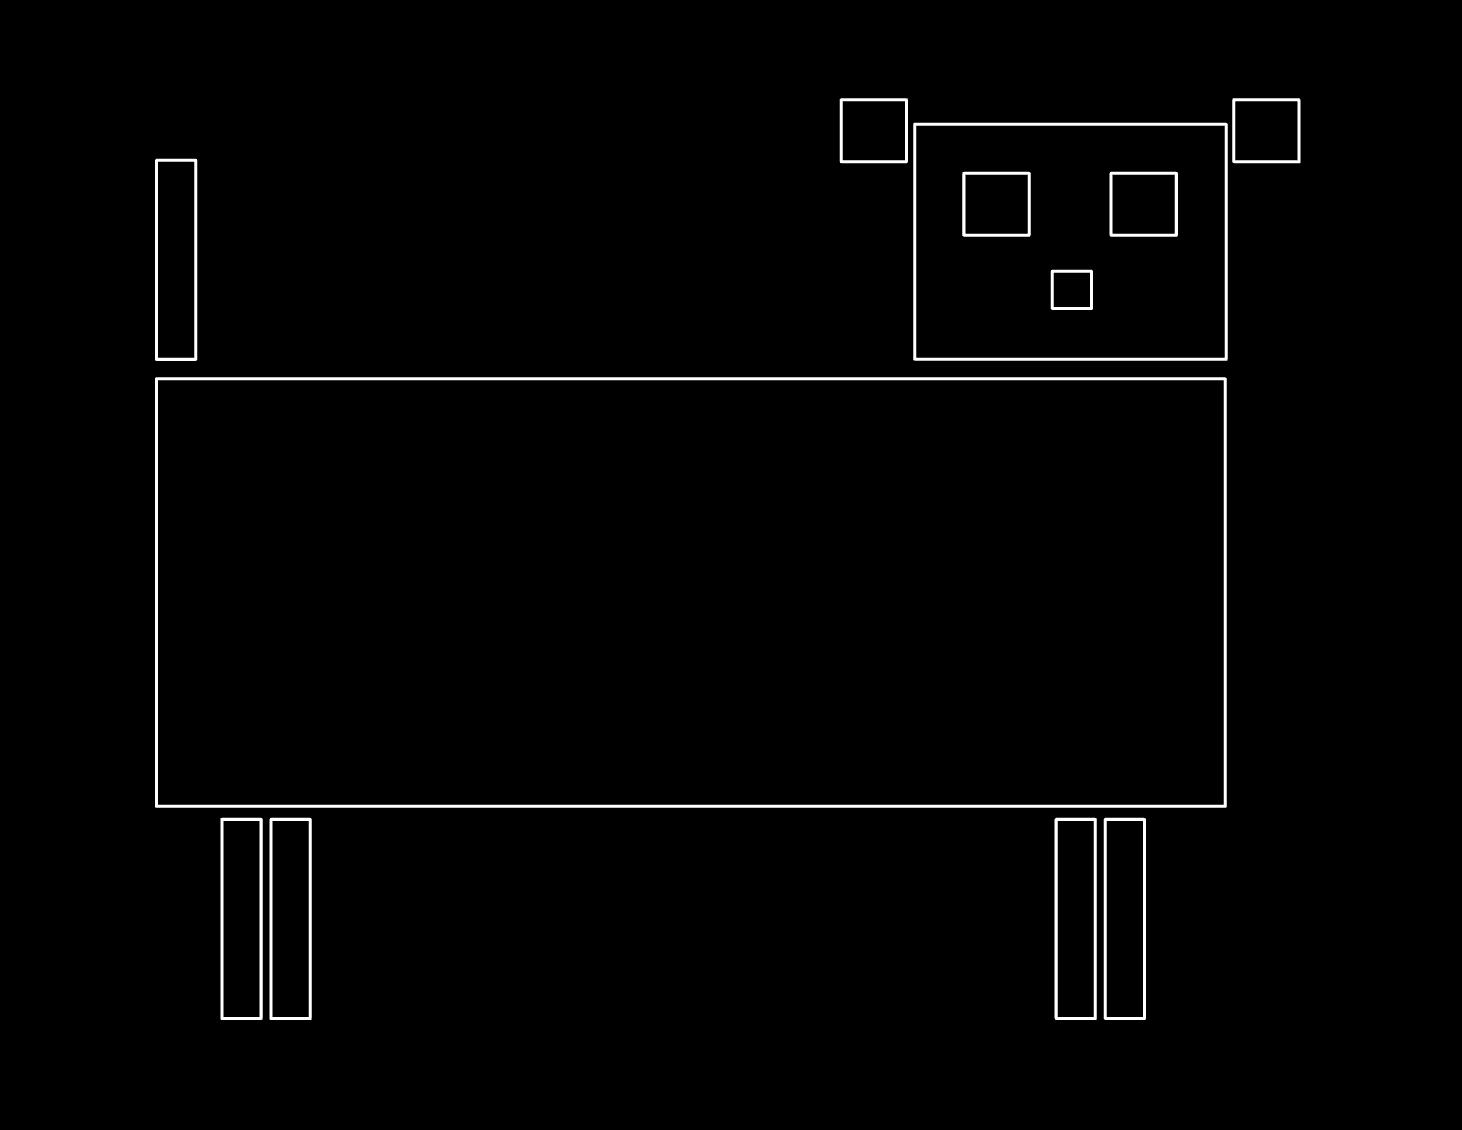
\includegraphics[width=5cm]{images/cat}
  \caption {Котка, нарисувана само с правоъгълници}
  \label{fig:cats}
  &
	\includegraphics[width=5cm]{images/pusheen}
  \caption {Pusheen the cat. Фигурата е от \cite{pusheen}}
\end{tabular}
\end{figure} 


  \item(*) \textit{Следната задача илюстрира метода на трапеците (Trapezoidal rule) за приближено изчисление на определени интеграли:}
	Да се нарисуват програмно координатни оси на евклидова координатна система с даден център в екранните координати (x,y). Да приемем, че в програмата е дефинирана функция \code {double f (double x)}, за която знаем, че е дефинирана за всяка стойност на $x$.
	\begin{itemize}
		\item Да се изобрази графиката на функцията спрямо нарисувана координатна система
		\item Да се приближи чрез трапеци с дадена дължина на основата $\delta$ фигурата, заключена между видимата графика на фигурата и абсцисата
		\item Да се визуализират така получените трапеци
		\item Да се изчисли сумата от лицата на така получените трапеци
		\item Да се експериментира с различни дефиниции на функцията $f$
	\end{itemize}

  За пример виж фигура \ref{fig:trapezoidal}.

\end{enumerate}


\clearpage\section {Цикли, масиви и низове}

\subsection {Цикли \textrm{II}}

Където не е посочено изрично, под ``редица от числа $a_0, a_1, ..., a_{n-1}$'' по-долу се разбира последователност от $n$ числа, въведени от стандартния вход. Задачите да се решат \emph{без} използването на масиви.


\begin{enumerate}[]


		\item Задача 3.1. \cite{sbornik} Да се напише програма, която въвежда редица от n цели числа $(1 \leq n \leq 50)$ и намира и извежда минималното от тях.

		\item Задача 3.2. \cite{sbornik} Да се напише програма, която въвежда редицата от n $(1 \leq n \leq 50)$ цели числа $a_0, a_1, ..., a_{n-1}$ и намира и извежда сумата на тези елементи на редицата, които се явяват удвоени нечетни числа.

		\item Задача 3.3. \cite{sbornik} Да се напише програма, която намира и извежда сумата от положителните и произведението на отрицателните елементи на редицата от реални числа $a_0, a_1, ..., a_{n-1}$ $(1 \leq n \leq 20)$.

		\item Задача 3.7. \cite{sbornik} Да се напише програма, която изяснява има ли в редицата от цели числа $a_0, a_1, ..., a_{n-1}$ $(1 \leq n \leq 100)$ поне два последователни елемента с равни стойности.

		\item Задача 3.8. \cite{sbornik} Да се напише програма, която проверява дали редицата от реални числа $a_0, a_1, ..., a_{n-1}$ $(1 \leq n \leq 100)$ е монотонно растяща.

    \item Задача 3.15. \cite{sbornik} Да се напише програма, която въвежда реалните вектори $a_0, a_1, ..., a_{n-1}$ и $b_0, b_1, ..., b_{n-1}$ $(1 \leq n \leq 100)$,  намира скаларното им произведение  и го извежда на екрана.

		\item Задача 3.10. \cite{sbornik} Да се напише програма, която за дадена числова редица $a_0, a_1, ..., a_{n-1}$ $(1 \leq n \leq 100)$ намира дължината на най-дългата ú ненамаляваща подредица $a_i, a_{i+1}, ..., a_{i+k}$ $(a_i \leq a_{i+1} \leq ... \leq a_{i+k})$.


\end{enumerate}

\subsection {Цикли и низове}
Където не е посочено изрично, под ``редица от символи $s_0, s_1, ..., s_{n-1}$ $(1 \leq n \leq 100)$ $a_0, a_1, ..., a_{n-1}$'' по-долу се разбира символен низ с дължина $n$, въведен от клавиатурата в масив от тип \code{char[255]}.

\begin{enumerate}[resume]


  \item Задача 3.11. \cite{sbornik}	Дадена е редицата от символи $s_0, s_1, ..., s_{n-1}$ $(1 \leq n \leq 100)$. Да се напише програма, която извежда отначало всички символи, които са цифри, след това всички символи, които са малки латински букви и накрая всички останали символи от редицата, запазвайки реда им в редицата.

	\item Задача 3.13. \cite{sbornik} Задача 3.13. Да се напише програма, която определя дали редицата от символи $s_0, s_1, ..., s_{n-1}$ $(1 \leq n \leq 100)$ е симетрична, т.е. четена отляво надясно и отдясно наляво е една и съща.

  \item Да се напише функция, която по два низа намира дължината на най-дългия им общ префикс. \textit{Префикс на низ наричаме подниз със същото начало като дадения. Пример: празният низ и низовете ``a'', ``ab'', и ``abc'' са всички възможни префикси на низа ``abc''. Дължината на най-дългия общ префикс на низовете ``abcde'' и ``abcuwz'' е 3.}

  \item Да се напише функция, която в даден низ замества всички малки латински букви със съответните им големи латински букви.

  \item Да се напише функция \code{reverse(s)}, която превръща даден низ в огледалния му образ. \textit{Например, низът ``abc'' ще се преобразува до ``cba''.}

  \item Да се напише функция, която по даден низ $s$, всички букви в който са латински, извършва следната манипулация над него: Ако $s$ съдържа повече малки, отколкото големи букви, замества всички големи букви в $s$ с малки. В останалите случаи, всички малки букви се заместват с големи.

	\item Задача 3.26. "Хистограма на символите" \cite{sbornik} Символен низ е съставен единствено от малки латински букви. Да се напише програма, която намира и извежда на екрана броя на срещанията на всяка от буквите на низа.

  \item Да се напише булева функция, която по дадени низове $s_1$ и $s_2$ проверява дали $s_2$ е подниз на $s_1$ (\textit{Например, низът ``uv'' е подниз на низовете ``abuvc'', ``uvz'', ``zuv'' и ``uv'', но не е подниз на низа ``uwv''}.). Функцията да \emph{не} използва вложени цикли.

  \item Задача 3.28. "Търсене на функция" \cite{sbornik} Дадени са два символни низа с еднаква дължина $s_1$ и $s_2$, съставени от малки латински букви. Да се напише програма, която проверява дали съществува функция $f:char \rightarrow char$, изобразяваща $s_1$ в $s_2$, така че $f(s_1[i])$ = $f(s_2[i])$ и $i=1..$дължината на $s_1$ и $s_2$. \textit{Упътване: За да е възможна такава функция, не трябва в $s_1$ да има символ, на който съответстват два или повече различни символи в $s_2$. Например, низът ``aba'' може да бъде изобразен в низа ``zwz``, но не и в низа ``zwu''.}

\end{enumerate}


\pagebreak

\subsection {Матрици и вложени цикли}

\begin{enumerate}[resume]

	\item Задача 3.18. \cite{sbornik} Дадени са числовите редици $a_0, a_1, ..., a_{n-1}$ и $b_0, b_1, ..., b_{n-1}$ $(1 \leq n \leq 50)$. Да се напише програма, която въвежда от клавиатурата двете редици и намира броя на равенствата от вида $a_i = b_j$ $(i = 0, ..., n-1, j = 0, ..., n-1)$.

	\item Задача 3.21. \cite{sbornik} Две числови редици си приличат, ако съвпадат множествата от числата, които ги съставят. Да се напише програма, която въвежда числовите редици $a_0, a_1, ..., a_{n-1}$ и $b_0, b_1, ..., b_{n-1}$ $(1 \leq n \leq 50)$ и установява дали си приличат.

	\item Задача 3.29. \cite{sbornik} Дадена е квадратна целочислена матрица A от n-ти ред $(1 \leq n \leq 50)$. Да се напише програма, която намира сумата от нечетните числа под главния диагонал на A (без него).

  \item Задача 3.45. \cite{sbornik} Матрицата А има седлова точка в $a_{i,j}$, ако $a_{i,j}$ е минимален елемент в i-тия ред и максимален елемент в j-тия стълб на A. Да се напише програма, която извежда всички седлови точки на дадена матрица А с размерност $n \times m (1 \leq n \leq 20, 1 \leq m \leq 30)$.

	\item Задача 3.113. (периодичност на масив). \cite{sbornik}	Да се напише програма, която проверява дали в едномерен масив от цели числа съществува период. Например, ако масивът е с елементи 1, 2, 3, 1, 2, 3, 1, 2, 3, 1, периодът е 3. Ако период съществува, да се изведе.

	\item Да се напише програма, която въвежда от клавиатурата матриците от цели числа $A_{N\times M}$ и $B_{M\times N}$ и извежда на екрана резултатът от умножението на двете матрици.


\end{enumerate}

\subsection {Елементарно сортиране на масиви}

\begin{enumerate}[resume]
  \item Да се реализира функция, сортираща масив по метода на мехурчето. При този метод масивът $a[0],..,a[n-1]$ се обхожда от началото към края, като на всяка стъпка се сравняват двойката съседни елементи $a[i]$ и $a[i+1]$. Ако $a[i+1] < a[i]$, местата им се разменят. Този процес се извършва $n$ пъти.
  \item Да се напише функция \code{unsortedness}, която оценява доколко един масив е несортиран като преброява колко от елементите му ``не са на местата си''. Т.е. функцията намира броя на тези елементи $a_i$, които не са $i$-ти по големина в масива. Например, за масива $\{0,2,1\}$ това число е $2$.
  \item Да се напише функция \code{swappable}, която за масива $a[0],..,a[n-1]$ проверява дали има такова число $i(0 < i < n-1)$, че масива $a_i,..,a_n,a_0,..,a_{i-1}$ е сортиран в нарастващ ред. Т.е. може ли масивът да се раздели на две части (незадължително с равна дължина) така, че ако частите се разменят, да се получи нареден масив. Пример за такъв масив е $\{3,4,5,1,2\}$.

\end{enumerate}

\begin{mdframed}[hidealllines=true,backgroundcolor=gray!20]
Функцията \code{std::clock()} от \code{<ctime>} връща в абстрактни единици времето, което е изминало от началото на изпълнение на програмата. Обикновено тази единица за време, наречена ``\code{tick}'', е фиксиран интервал ``реално'' време, който зависи от хардуера на системата и конфирграцията ѝ. Константата \code{CLOCKS\_PER\_SEC} дава броя \code{tick}-ове, които се съдържат в една секунда реално време.

Чрез следния примерен код може да се измери в милисекунди времето за изпълнение на програмния блок, обозначен с ``...''.
\begin{verbatim}
clock_t start = std::clock();
//...
clock_t end = std::clock();

long milliseconds = (double)(end-start)/
                    (CLOCKS_PER_SEC/1000.0);

\end{verbatim}
\end{mdframed}
\begin{mdframed}[hidealllines=true,backgroundcolor=gray!20]
Функцията \code{rand()} от \code{<cstdlib>} генерира редица от псевдо-случайни числа. Всяко последователно изпълнение на функцията генерира следващото число от редицата. За да се осигури, че при всяко изпълнение на програмата ще се генерира различна редица от псевдо-случайни числа, е необходимо да се изпълни функцията \code{srand()} с параметър, който е различен за всяко изпълнение на програмата. Една лесна възможност е да се ползва резултата на функцията \code{time(0)}, която дава текущото време на системния часовник в стандарт \code{epoch time}. Достатъчно е \code{srand()} да се изпълни веднъж за цялото изпълнение на програмата.

Чрез следния примерен код може да се генерира редица от 10 (практически) случайни числа, които са различни при всяко изпълнение на програмата.
\begin{verbatim}
srand (time(0));
for (int i = 0; i < 10; i++)
{
  std::cout << rand () << std::endl;
}
\end{verbatim}
Стойностите на \code{rand()} са в интервала $[0..INT\_MAX]$. Ако е нужно да генерирате стойности в друг интервал, например $[0..N]$, това може да стане по формулата $\frac{rand()}{INT\_MAX}\times N$ (трябва да избегнете целочисленото делене)!
\end{mdframed}

\begin{enumerate}[resume]

  \item Да се измери емпирично времето за изпълнение на алгоритъма за сортиране по метода на мехурчето. Да се начертае графика на зависимостта на времето за изпълнение от големината на масива. Всеки тест да е с наново генериран масив от случайни числа.
  \item Да се въведе матрица от числа $A_{N \times M}$.
  \begin{itemize}
      \item Да се сортира всеки от редовете на матрицата
      \item Да се сортира всяка от колоните на матрицата
  \end{itemize}
  Така получените матрици да се отпечатат на стандартния изход.

\end{enumerate}



\begin{mdframed}[hidealllines=true,backgroundcolor=gray!20]
\code{Bozosort} е случайностен алгоритъм за сортиране на масиви. При този алгоритъм, на всяка стъпка се разменят две случайни числа от масива, след което се проверява дали масивът се е сортирал. Процесът продължава до сортиране на масива.
\end{mdframed}

\begin{enumerate}[resume]

  \item Да се реализира алгоритъма \code{Bozosort}. Да се измери емпирично времето му за изпълнение. \emph{Внимание: тествайте с достатъчно малки масиви, тъй като този алгоритъм е изключително бавен.}

\end{enumerate}

\subsection {Низове II}

\begin{itemize}[resume]

  \item Задача 3.55. \cite{sbornik} Дадена е квадратна таблица $A_{n\times n}$ $(1 \le n \le 30)$ от низове, съдържащи думи с максимална дължина 6. Да се напише програма, която проверява дали изречението, получено след конкатенацията на думите от главния диагонал (започващо от горния ляв ъгъл) съвпада с изречението, получено след конкатенацията на думите от вторичния главен диагонал на A (започващо от долния ляв ъгъл).

  \item Задача 3.56. \cite{sbornik} Дадена е квадратна таблица A от n-ти ред $(1 \le n \le 20)$ от низове, съдържащи думи с максимална дължина 9. Да се напише програма, която намира и извежда на екрана изречението, получено след обхождане на A по спирала в посока на движението на часовниковата стрелка, започвайки от горния ляв ъгъл. Например ако матрицата A има вида:

  $\left( \begin{array}{ccc}
  a & b & c \\
  d & e & f \\
  g & h & i
  \end{array} \right)$

  изречението след обхождането по спирала е: ``abcfihgde''.

  \item Задача 3.57 (Inner Join). \cite{sbornik} Нека са дадени два масива от низове – students и grades с най-много 20 низа във всеки. Низовете в масива students имат вида ``XXXXXX YYYY...'', където ``XXXXXX'' е шестцифрен факултетен номер, а ``YYYY...'' е име с произволна дължина. Низовете в grades имат вида ``XXXXXX YYYY'', където ``XXXXXX'' е шестцифрен факултетен номер, а ``YYYY'' е оценка под формата на число с плаваща запетая. И двата масива са сортирани във възходящ ред по факултетен номер. Възможно е в някой от двата масива да има данни за факултетни номера, за които няма данни в другия. И в двата списъка даден факултетен номер се среща най-много един път. Да се напише програма, която извежда на екрана имената и оценките на тези студенти, за които има информация и в двата списъка, като оценките са увеличени с 1 единица, но са максимум 6.00.

\end{itemize}

\subsection{Инвариант на цикъл и верификация на програми}

\emph{Изложението в тази секция е силно опростена версия на метода на Флойд (Floyd) за верификация на блок схеми, описан в монументалната му статия \cite{floyd}. Редица идеи и задачи са взаимствани от книгата \cite{tpsbornik} на А. Соскова и С. Николова ``Теория на програмите в задачи''. За по-подробно изложение и допълнителни примери и задачи препоръчваме тази книга. Изложението по-долу е нарочно опростено, като на места е жертвана прецизността му.}

\begin{mdframed}[hidealllines=true,backgroundcolor=gray!20]


\bigskip
\textbf{Инвариант на цикъл}
\bigskip


Нека е дадена програма или част от програма, която се се състои от единствен \code{while} цикъл. Нека имаме някакъв набор от работни променливи $v_1,..,v_n$, които се инициализират непосредствено преди \code {while} цикъла. Условието на цикъла зависи изцяло от работните променливи, а тялото на цикъла използва или променя само тях. Приемаме, че програмата не произвежда странични ефекти и не зависи от такива.

Тоест, за програмата знаем, че: (1) не извършва входни и изходни операции, (2) поведението ѝ зависи изцяло от началните стойности на работните променливи $v_1,..,v_n$ и (3) не модифицира никакви други променливи, освен работните. Такава програма можем да изобразим чрез блок схемата на Фигура \ref{fig:1while}.
\end{mdframed}


\begin{figure}
    \begin{tikzpicture}[auto, node distance=1.5cm,>=latex']
    \node [entry, name=start](start){};
    \node [block,name=init, below of = start] (init)
       {Инициализация на\\ $v_0,..,v_n$};
    \node [fork,name=test1fork,below of = init,node distance = 2cm]{};
    \node [condition,name=test1, below of = test1fork,node distance = 3cm] (test1) {Условие \\ $C(v_0,..,v_n)$};
    \node [block,name=inc,right of = test1, node distance = 6.5cm] (inc) {Операции \\$(v_0^i,..,v_n^i) \rightarrow (v_0^{i+1},..,v_n^{i+1})$};
    \node [fork,name=endfork,below of = test1, node distance = 3cm]{};
    \node [entry, name=end, below of = endfork, node distance = 1cm](end){};

    \node [name=cut1, left of = test1fork, node distance = 2cm](cut1){1};
    \node [name=cut2, left of = endfork, node distance = 2cm](cut2){2};

    \draw [->] (start) -- (init);
    \draw [-] (init) -- (test1fork);
    \draw [->] (test1fork) -- (test1);
    \draw [->] (test1) -- node{true} (inc);
    \draw [->] (inc) |- (test1fork);
    \draw [-] (test1) -- node []{false}(endfork);
    \draw [->] (endfork) -- (end);

    \draw [-,dashed] (cut1) -- (test1fork);
    \draw [-,dashed] (cut2) -- (endfork);
    \end{tikzpicture}

  \caption{Блок схема на част от програма с \code{while} цикъл}
  \label{fig:1while}
\end{figure}


\begin{mdframed}[hidealllines=true,backgroundcolor=gray!20]
На фигурата $C(v_1,..,v_n)$ е някакъв логически израз, зависещ само от $v_1,..,v_n$. Да допуснем, че сме ``замразили'' изпълнението на програмата в точката, обозначена с ``1'', точно преди да започне $i$-тото поред ($i\geq 0$) изпълнение на тялото на цикъла, т.е. непосредствено преди да бъдат изпълнени операторите в него за $i$-ти път. В този момент $n$-торката работни променливи $(v_1,..,v_n)$ имат някакви конкретни стойности. Да ги обозначим с $(v_0^{i},..,v_n^{i})$. След изпълнение на всички оператори в тялото на цикъла работните променливи получават някакви нови стойности. Това са точно стойностите $(v_0^{i+1},..,v_n^{i+1})$, които работните променливи ще имат в началото на $i+1$-вата итерация. Това е изобразено на фигурата чрез прехода $(v_0^i,..,v_n^i) \rightarrow (v_0^{i+1},..,v_n^{i+1})$.

Нека приемем, че при някакво конкретно изпълнение на програмата, при конкретни дадени начални стойности на работните променливи  $(v_0^{0},..,v_n^{0})$, тялото на цикъла ще бъде изпълнено точно  $k\geq 0$ пъти, след което условието $C(v_1,..,v_n)$ на цикъла ще се наруши и той ще приключи. Изпълнението на програмата достига точката, обозначена с ``2''. По този начин се получава редицата от $n$-торки $(v_0^{0},..,v_n^{0}),..,(v_0^{k},..,v_n^{k})$, като за всички нейни членове $0\leq i < k$, освен за последния, знаем че е вярно $C(v_0^{i},..,v_n^{i})$, а за последния, $k$-ти член, е вярно обратното --- $\neg C(v_0^{k},..,v_n^{k})$.

Освен свойството $C(v_0^{i},..,v_n^{i})$ (или неговото отрицание), което знаем за всички последователни стойности на работните променливи, можем да въведем още едно свойство $I(v_0^{i},..,v_n^{i})$, наречено ``инвариант на цикъла''. За свойството $I$ искаме да е вярно за всички възможни стойности на работните променливи, дори и за последния член на редицата им. От там идва името ``инвариант'', т.е. факт, което е винаги верен.

Това свойство може да е произволно, например тъждествената истина \code{true} изпълнява условието за инвариант, тъй като е вярна за всички членове на редицата на работните променливи. Инвариантът обаче е най-полезен, когато представя ``смисъла'' на работните променливи, и ако от верността на $\neg C(v_0^{k},..,v_n^{k})\,\&\, I(v_0^{k},..,v_n^{k})$ можем да изведем нещо полезно за ``крайния резултат'' от изпълнението на цикъла, съдържащ се в стойностите $(v_0^{k},..,v_n^{k})$.
\end{mdframed}

\begin{figure}
    \begin{tikzpicture}[auto, node distance=1.5cm,>=latex']
    \node [entry, name=start](start){};
    \node [block,name=init, below of = start, align=left] (init)
       {\code{candidate = 0;}\\\code{current = 1;}};

    \node [fork,name=test1fork,below of = init,node distance = 2cm]{};

    \node [block,name=inc2, right of = test1fork, node distance = 5cm,minimum height=1.5cm]{\code{current++;}};

    \node [condition,name=test1, below of = test1fork,node distance = 3cm] (test1) {\code{current < m}};

    \node [condition, name=test2, right of = test1, node distance = 5cm,font=\tiny] (test2) {\code{A[current]}\\\code{<A[candidate]}};

    \node [block,name=inc,right of = test2, node distance = 5cm, minimum height=1.5cm] (inc) {\code{candidate = current};};

    \node [fork,name=endfork,below of = test1, node distance = 3cm]{};
    \node [entry, name=end, below of = endfork, node distance = 1cm](end){};

    \node [name=cut1, left of = test1fork, node distance = 2cm](cut1){1};
    \node [name=cut2, left of = endfork, node distance = 2cm](cut2){2};

    \draw [->] (start) -- (init);
    \draw [-] (init) -- (test1fork);
    \draw [->] (test1fork) -- (test1);

    \draw [->] (test1) -- node{true} (test2);
    \draw [->] (test2) -- node{true} (inc);

    \draw [->] (inc) |- (inc2);
    \draw [->] (inc2) -- (test1fork);
    \draw [->] (test2) -- node{false} (inc2);


    \draw [-] (test1) -- node []{false}(endfork);
    \draw [->] (endfork) -- (end);

    \draw [-,dashed] (cut1) -- (test1fork);
    \draw [-,dashed] (cut2) -- (endfork);
    \end{tikzpicture}

  \caption{Блок схема на програмата за намиране на най-малък елемент в масив}
  \label{fig:minel}
\end{figure}



\begin{mdframed}[hidealllines=true,backgroundcolor=gray!20]

\bigskip
\textbf{Верификация на програми}
\bigskip

Понятието ``инвариант'' ще илюстрираме чрез едно негово приложение: ``Верификация на програма''. Верификацията на програма е доказателство, че при необходимите начални условия дадена програма изчислява стойност, удовлетворяваща някакво желано свойство. Като пример да разгледаме следната  програма, за която ще се уверим, че намира най-малък елемент на едномерен масив $A$ с $m>0$ елемента $A[0],..,A[m-1]$.


\begin{verbatim}
size_t candidate = 0, current = 1;
while (current < m)
{
  if (A[candidate] < a[current])
  {
    candidate = current;
  }
  current++;
}
\end{verbatim}
Можем да приложим метода на инварианта, за да докажем строго, че когато цикълът приключи, то елементът $A[candidate]$ е гарантирано по-малък или равен на всички останали елементи на масива.
Като първа стъпка, за улеснение изобразяваме програмата като блок схемата на Фигура \ref{fig:minel}.


Работните променливи на програмата, освен масива $A$, са целочислените променливи \code{candidate} и \code{current}. Какъв е смисълът на тези променливи? Веднага се вижда, че \code{current} е просто брояч --- служи за обхождане на елементите на масива последователно от $A[0]$ до $A[m-1]$, като на всяка итерация от цикъла се разглежда стойността на $A[current]$.

Интуитивно се вижда, че \code{candidate} е намереният най-малък елемент на масива до текущия момент от обхождането. Тоест, можем да се надяваме, че ако сме разгледали първите $i$ елемента на масива, то правилно сме определили, че най-малкият от тях е $A[current]$.

Тези размишления може да запишем чрез инварианта:

$I ::= A[candidate]=min(A[0],..,A[current-1])$.

Този инвариант очевидно е верен в началото на изпълнението на програмата, когато $current=1$, а $candidate=0$. Как да се уверим, че инвариантът е валиден за всички стойности, през които преминават работните променливи?

Нека допуснем, че инвариантът е верен за някаква стъпка $i$ от изпълнението на цикъла. Тоест, допускаме $I(candidate^i, current^i)$, или $A[candidate^i]=min(A[0],..,A[current^i-1])$.

На итерация $i+1$ имаме  и $current^{i+1}=current^{i}+1$, и следователно трябва да покажем, че $A[candidate^{i+1}]=min(A[0],..,A[current^{i+1}-1])$.

След навлизане в тялото на цикъла, имаме две възможности:
\begin{enumerate}[label=\arabic*)]
  \item $A[current^i]\geq A[candidate^i]$. От допускането следва, че добавянето на $A[current^i]$ към $min(A[0],..,A[current^i-1])$ не променя стойността на минимума, или $min(A[0],..,A[current^i-1])=min(A[0],..,A[current^i-1],A[current^i])$. От тук директно се вижда, че инвариантът е верен за итерация $i+1$.
  \item $A[current^i] < A[candidate^i$]. Тъй като по допускане $A[candidate^i] = min(A[0], .., A[current^i-1])$, от тук следва, че $A[current^i] < min(A[0], .., A[current^i-1])$, следователно

   $A[current^i] = min(A[0], .., A[current^i-1], A[current^i])$.

   Но след присвояването имаме $candidate^{i+1} = current^i$, от където $A[candidate^{i+1}] = min(A[0],..,A[current^i])$. Но $current^i = current^{i+1}-1$, от където получаваме верността на $I$ за итерация $i+1$: $A[candidate^{i+1}] = min(A[0], .., A[current^{i+1}-1])$.

\end{enumerate}
  Доказателството протича по индукция. Уверяваме се, че инвариантът е верен за цялата редица от стойности на \code{candidate} и \code{current}.

  Какво се случва в края на цикъла, когато имаме $\neg(current<m)$? Тъй като числата са цели, а \code{current} се увеличава само с единица, можем да заключим, че $current=m$. Замествайки това равенство в инварианта, получаваме твърдението

  $A[candidate] = min(A[0], .., A[m-1])$.

  Тоест, намерили сме минималния елемент на масива.
\end{mdframed}

\begin{enumerate}[resume]
  \item Да се докаже строго, че за следната функция е вярно $pow(x,y)=x^y$:
  \begin{enumerate}[label=\alph*)]%[a)] % a), b), c), ...

    \item
\begin{verbatim}
unsigned int pow (unsigned int x, usnigned int y)
{
  unsigned int p = 1, i = 0;
  while (i < y)
  {
    p *= x;
    i++;
  }
  return p;
}
\end{verbatim}
    \item
\begin{verbatim}
unsigned int pow (unsigned int x, usnigned int y)
{
  unsigned int p = 1;
  while (y > 0)
  {
    p *= x;
    y--;
  }
  return p;
}
\end{verbatim}
      \item
\begin{verbatim}
unsigned int pow (unsigned int x, usnigned int y)
{
  unsigned int z = x, t = y, p = 1;
  while (t > 0)
  {
    if (t%2 == 0)
    {
      z *= z;
      t /= 2;
    }else{
      t = t - 1;
      p *= z;
    }
  }
  return p;
}
\end{verbatim}
  \end{enumerate}

  \item Да се докаже строго, че за следната функция е вярно $sqrt(n)=[\sqrt{n}]$.

\begin{verbatim}
unsigned int sqrt (unsigned int n)
{
  unsigned int x = 0, y = 1, s = 1;
  while (s <= n)
  {
    x++;
    y += 2;
    s += y;
  }
  return x;
}
\end{verbatim}

\item Да се напише програма, която проверява дали дадени два масива $A$ и $B$ с еднакъв брой елементи $m$ са еднакви, т.е. съдържат същите елементи в същия ред. Да се докаже строго, че програмата работи правилно.

\item Да се докаже, че следната функция връща истина тогава и само тогава, когато масивът \code{A} с \code{n} елемента съдържа елемента \code{x}.

\begin{verbatim}
bool member (int A[], size_t n, int x)
{
  size_t i = 0;
  while (i < n && A[i] != x)
  {
    i++;
  }
  return i < n;
}
\end{verbatim}

\item Да се напише програма, която проверява дали даден масив $A$ с $m$ елемента е сортиран, т.е. дали елементите му са наредени в нарастващ ред. Да се докаже строго, че програмата работи правилно.

\end{enumerate}

\begin{mdframed}[hidealllines=true,backgroundcolor=gray!20]
Съществуват редица съвременни методи за верификация на програми. Пълната версия на метода, използван по-горе, се нарича ``логика на Флойд-Хоар'' (Floyd–Hoare logic) и е само един представител на този клас методи.

Също така, в компютърните науки има направление, наречено ``Синтез на програми'' (Program refinement). При синтеза на програми се решава обратната задача: по спецификация на входа и изхода да се генерира програма, която удовлетворява спецификацията.

Препоръчваме на любознателния читател да се запознае с логиката на Floyd–Hoare и методите за синтез на програми.
\end{mdframed}

\pagebreak

\clearpage\section{Указатели и програмен стек}

\subsection {Предаване на масиви и указатели като параметри на функции}
\begin{enumerate}
  \item Да се дефинира функция, която получава като параметри два масива с еднакъв брой елементи. Функцията да разменя съответните елементи на масивите ($a[i] \leftrightarrow b[i]$).
  \item Да се дефинира функция \texttt{swap([подходящ тип] a,[подходящ тип] b)}, която разменя стойностите на две целочислени променливи, предадени на функцията чрез a и b.

  \emph{Каква е разликата с предишната задача? Защо при тази задача се налага използване на псевдоними?}
\end{enumerate}

\subsection {Масиви от указатели}
\begin{enumerate}[resume]
  \item Да се напише булева функция \code{bool duplicates (long *ponters[])}, която получава като параметър масив \code{pointers} от указатели към целочислени променливи. Функцията да проверява дали поне две от съответните променливи имат еднакви стойности.
  \item Да се дефинира функцията  \texttt{bool commonel (int *arrays[],int npointers, int arrlengths[])}. Масивът \texttt{arrays} съдържа \texttt{npointers} на брой указатели към масиви от цели числа. \texttt{i}-тият масив има големина \texttt{arrlengths[i]}. Функцията да връща истина, ако има поне едно число $x$, което е елемент на всички масиви.
  \item Да се дефинира функцията \texttt{bool subarrays (int *arrays[],int npointers, int arrlengths[])}. Масивът \texttt{arrays} съдържа \texttt{npointers} на брой указатели към масиви от цели числа. \texttt{i}-тият масив има големина \texttt{arrlengths[i]}. Функцията да връща истина, ако поне един от масивите е подмасив на друг масив. Масивът $a$ наричаме подмасив на $b$, ако заетата от $a$ памет е част от заетата от $b$ памет. Да се напишат подходящи тестове за функцията.
\end{enumerate}

\subsection {Програмен стек}
\begin{enumerate}[resume]
  \item Да се дефинира рекурсивна функция \code{double sum(size\_t n)}, която въвежда $n$ числа от стандартния вход връща сумата им. \emph{Да не се използват оператори за цикъл!}

  \item Да се дефинира рекурсивна функция \code{reverse(n)}, която въвежда $n$ числа от стандартния вход и ги извежда в обратен ред. \emph{Да не се използват масиви. Да се използва програмния стек чрез рекурсия.}

  \item Да се дефинира функция \code{void getmax (long *pmax, size\_t n)}, която въвежда $n$ числа от стандартния вход и записва максималното от тях в променливата, сочена от указателя \code{pmax}.

  Пример: Следната програма ще изведе най-малкото от 5 въведени от стандартния вход числа.
  \begin{verbatim}
  int main ()
  {
    long max = -1;
    getmax (&max,5);
    std::cout << max;

    return 0;
  }
  \end{verbatim}
  \emph{Функцията да се реализира по два начина: чрез цикъл и чрез използване на рекурсия без оператори за цикъл.}
\end{enumerate}

\pagebreak

\clearpage\section {Рекурсия}
\subsection {Прости рекурсивни функции}

\begin{enumerate}

	\item Задача 5.2.\cite{sbornik} Да се дефинира рекурсивна функция за намиране на стойността на полинома на Ермит $Hn(x)$ (x е реална променлива, а n неотрицателна цяла променлива), дефиниран по следния начин:

	$H_0(x)=1$

	$H_1(x)=2x$

	$H_n(x)=2xH_{n-1}(x)+2(n-1)H_{n-2}(x), n>1$


	\item Задача 5.3.\cite{sbornik} Произведението на две положителни цели числа може да се дефинира по
следния начин:

	$mult (m,n) = m$, ако n = 1

	$mult (m,n) = m + mult (m,n-1)$, иначе.

	Да се дефинира рекурсивна функция, която намира произведението на две положителни цели числа по описания по-горе начин.

	\item Задача 5.5.\cite{sbornik} Да се дефинира функция, която намира най-големия общ делител на две неотрицателни цели числа, поне едното от които е различно от 0.

	\item Задача 5.7.\cite{sbornik} Дадени са естествените числа n и k $(n \ge 1, k > 1)$. Да се дефинира рекурсивна функция, която намира произведението на естествените числа от 1 до n със стъпка k.

	\item Задача 5.10.\cite{sbornik} Дадено е неотрицателно цяло число n в десетична бройна система. Да се дефинира рекурсивна функция, която намира сумата от цифрите на n в бройна система с основа k $(k > 1)$.

	\item Задача 5.11.\cite{sbornik} Да се дефинира рекурсивна функция, която установява дали в записа на неотрицателното цяло число n, записано в десетична бройна система, се съдържа цифрата k.

	\item Задача 5.19.\cite{sbornik} Да се дефинира рекурсивна функция, която проверява дали дадено положително цяло число е елемент на редицата на Фибоначи.

	\item Задача 5.28.\cite{sbornik} Да се дефинира рекурсивна функция, която намира максималния елемент на редицата от цели числа $a_0, a_1, a_2, ..., a_{n-1}$, където $n \ge 1$.

	Забележка: Редицата е представена като масив.

	\item Задача 5.31.\cite{sbornik} Да се напише функция

	\texttt{void insertSorted (long x, long arr[], long n)},

	която включва цялото число \texttt{x} число в сортирана във възходящ ред редица от цели числа \texttt{arr}, в която има записани \texttt{n} елемента. Вмъкването да запазва наредбата на елементите. Предполага се, че за редицата е заделена достатъчно памет за допълване с още едно число.

	\item Задача 5.34.\cite{sbornik} Да се дефинира рекурсивна функция, която сравнява лексикографски два символни низа.
\end{enumerate}

\subsection{Търсене с пълно изчерпване}


\begin{figure}
\includegraphics[width=15cm]{images/path1}
\vspace{-200px}
\caption{Примерени лабиринти}
\label{fig:samplelab}
\end{figure}


\begin{enumerate}[resume]

	\item \label{zad:labds} Нека е дадена квадратна матрица от цели числа $N \times N$, представяща ``лабиринт''. Елементи на матрицата със стойност $0$ смятаме за ``проходими'', а всички останали - за ``непроходими''. Път в лабиринта наричаме всяка последователност от проходими елементи на матрицата, които са съседни вертикално или хоризонтално, такава че (1) никой елемент от последователността не е последван директно от предшественика си (забранено е ``връщането назад'') и (2) най-много един елемент на последователността се среща в нея повече от веднъж (има най-много един ``цикъл'').

	Да се дефинира функция \texttt{bool downstairs (int sx, int sy, int tx, int ty)}, която проверява дали съществува път от елемента $(sx,sy)$ до елемента $(tx,ty)$, такъв, че всеки следващ елемент от пътя е или вдясно, или под предишния. Такъв път да наричаме ``низходящ''.

	Пример: На Фигура \ref{fig:samplelab}(а) такъв път съществува от елемента $(0,2)$ до елемента $(3,3)$, но не и от $(3,1)$ до $(0,0)$.

	\item При условията на дефинициите от предишната задача, да се дефинира функция \texttt{bool connected()}, която проверява дали от всеки елемент на матрицата $(sx,sy)$ до всеки елемент на матрицата  $(tx,ty)$, такива, че $sx \leq tx$ и $sy \leq ty$, съществува низходящ път.

	Пример: За лабиринта от Фигура \ref{fig:samplelab}(а) условието е изпълнено, но не и за лабиринта от Фигура \ref{fig:samplelab}(б).


	\item Да се напише програма, която по въведени от клавиатурата $4 \le n \le 8$ и $0 \le k \le n$ намира извежда на екрана всички възможни конфигурации на абстрактна шахматна дъска с размери $n \times n$ с разположени на нея $k$ коня така, че никоя фигура не е поставена на поле, което се ``бие'' от друга фигура според съответните шахматни правила.

	Пример за отпечатана конфигурация с $n=5, k=2$:
	\begin{verbatim}
	_ _ _ _ _
	_ _ H _ _
	_ _ _ _ _
	_ _ _ _ H
	_ _ _ _ _

	\end{verbatim}


	\item При условията на задача \ref{zad:labds} да се напише функция

	\texttt{int minDistance (int sx, int sy, int tx, int ty)},

	която по въведени от клавиатурата координати на елементи $s=(sx,sy)$ и $t=(tx,ty)$ намира \textit {дължината} на най-краткия път между $s$ и $t$. Обърнете внимание, че се иска \textit{път}, а не просто низходящ път.

	\item

	При условията на задача \ref{zad:labds} да се напише функция, която по въведени от клавиатурата координати на елементи $s=(sx,sy)$ и $t=(tx,ty)$ намира и отпечатва на екрана елементите, от които се състои най-краткия път между $s$ и $t$. Обърнете внимание, че се иска \textit{път}, а не просто низходящ път.


	\item Пъзел на Синди\cite{cindy}.

	Дадена е игрова дъска като на фигура 2, която се състои от $n$ черни и $n$ бели фигури. Фигурите могат да бъдат разположени на $2n+1$ различни позиции. Играта започва с разполагане на всички черни фигури вляво, а всички бели - вдясно на дъската.

	Черните фигури могат да се местят само надясно, а белите - само наляво. На всеки ход важат следните правила:


	\begin{itemize}
		\item всяка фигура се мести само с по една позиция, ако съответната позиция не е заета;
		\item ако позицията е заета, фигурата $X$ може да прескочи точно една фигура $Y$ от противоположния цвят, ако позицията след $Y$ e свободна.
	\end{itemize}

	Да се напише програма, която по въведено число $n$ отпечатва на екрана инструкции за игра така, че в края на играта всички бели фигури да са вляво на дъската, а всички черни - вдясно. Инструкциите да са от следния вид:

	\begin{verbatim}
		...
		Преместете черна фигура фигура от позиция 1 на позиция 2.
		Преместете бяла фигура от позиция 5 на позиция 3.
		...
	\end{verbatim}

	Допустимо е инструкциите да бъдат отпечатани в обратен ред.


	\begin{mdframed}[hidealllines=true,backgroundcolor=gray!20]

		На следните фигури е даден пример за игра:

		\begin{flushleft}
		\includegraphics[width=5cm]{images/step0}

		\relscale{0.8}
		1. Начална конфигурация.
		\end{flushleft}


		\begin{flushleft}
		\includegraphics[width=5cm]{images/step1}

		\relscale{0.8}
		2. Преместване на черна фигура с един ход надясно.
		\end{flushleft}

		\begin{flushleft}
		\includegraphics[width=5cm]{images/step2}

		\relscale{0.8}
		3. Преместване на бяла фигура с прескачане.
		\end{flushleft}

		\begin{flushleft}
		\includegraphics[width=5cm]{images/step3}

		\relscale{0.8}
		4. Преместване на черна фигура с един ход надясно.
		\end{flushleft}

		\begin{flushleft}
		\includegraphics[width=5cm]{images/step4}

		\relscale{0.8}
		5. Преместване на черна фигура чрез прескачане
		\end{flushleft}

		След ход 5 конфигурацията на играта е безперспективна.

	\end{mdframed}

\end{enumerate}

\subsection{Рекурсивен парсер}


\begin{mdframed}[hidealllines=true,backgroundcolor=gray!20]
По време на лекции разработваме лексически анализатор, рекурсивен парсер и интепретатор на прост език, състоящ се от аритметични изрази от следния вид:
\begin{flushleft}
  \relscale{0.7}
  \begin{lstlisting}[mathescape]
  <expression> ::= <number> | (<expression> <operator> <exprerssion>)
  <number> ::= {0,..,9}+
  <operator> ::= + | - | * | /
  \end{lstlisting}
\end{flushleft}

За двата вида възнможни изрази -- числова константа и приложение на двуместен аритметичен оператор, оградено в скоби -- дефинираме съответно класовете \code{ExprConstant} и \code{ExprOperator}, представящи изразите в синтактично дърво. Двата класа са наследници на абстрактен базов клас \code{Expression}, дефиниращ основаната операция \code{value} за намиране на оценка на израз.

Езикът разширяваме с условен оператор от вида:
\begin{flushleft}
  \relscale{0.6}
  \begin{lstlisting}[mathescape]
<expression> ::= ... | if <expression> than <expression> else <expression>
  \end{lstlisting}
\end{flushleft}

Изразите от този вид се представят в синтактичното дърво с обекти от клас \code{ExprIf}, съдържащ три член данни от тип \code{Expression*}, \code{condition}, \code{expthen} и \code{exprelse}. Методът \code{value} върща оценката на \code{expthen} или \code{exprelse} в зависимост от оценката на \code{condition}.
\end{mdframed}

\begin{enumerate}[resume]
\item Интерпретаторът на аритметични изрази от лекции да се разшири с възможност за групиране на изрази в ``блокове'', започващи с ключовата дума \code{begin} и завършващи с ключовата дума \code{end}:
\begin{flushleft}
  \relscale{0.7}
  \begin{lstlisting}[mathescape]
<expression> ::= ... | begin (<expression>;)+ end
  \end{lstlisting}
\end{flushleft}

Оценката на блок от изрази да се състои в последоватлено оценяване на всички изрази в блока и използване на онцеката на последния израз от блока като оценка на целия блок. Например: \code{begin 1; 2; 3; end} има оценка $3$.

\item Интерпретаторът на аритметични изрази от лекции да се разшири с възможност за извеждане на стойност на израз на стандартния изход:
\begin{flushleft}
  \relscale{0.7}
  \begin{lstlisting}[mathescape]
<expression> ::= ... | print <exprression>
  \end{lstlisting}
\end{flushleft}

Оценката на израз от типа \code{print e} се намира като оценката на израза \code{e}, като освен това се произвежда извеждане на страндартния изход като страничен ефект. Всяка отделна стайност да бъде изведена на нов ред.

Примрер: Оценката на израза \code{print 1} ще е $1$ и ще доведе до извежане на ``1'' на стандарния изход. Оценката на 

\begin{flushleft}
  \relscale{0.7}
  \begin{lstlisting}[mathescape]
begin 
   print 1; 
   print 2; 
   print begin 3; 4; end;
end
  \end{lstlisting}
\end{flushleft}
ще доведе до извеждане на следните редове на стандартния изход: 
\begin{flushleft}
  \relscale{0.7}
  \begin{lstlisting}[mathescape]
1
2
4
  \end{lstlisting}
\end{flushleft}

\item Нека е дадена следната граматика на език за програмиране, зададена чрез BNF:

\begin{flushleft}
\relscale{0.7}
\begin{lstlisting}[mathescape]
<program> ::= (<statement>;)$^+$
<statement> ::= <assignment> | <output>
<assignment> ::= set <variable> = <expression>
<output> ::= print <expression>
<variable> ::= a..z
<expression> ::= <variable> | <number> | <complex-expr>
<complex-exp> ::= <expression>(<operator> <expression>)$^*$ 
<complex-exp> ::=(<expression>(<operator> <expression>)$^+$)
<operator> ::= + | - | * | /
\end{lstlisting}
\end{flushleft}

Примерни програми на този език и съответния резултат на стандартния изход са:
\begin{lstlisting}[mathescape]
  print 10;
\end{lstlisting}
\emph{Изход:} 10

\begin{lstlisting}[mathescape]
  set x = 3*(1+2);
  print x + 10;
\end{lstlisting}
\emph{Изход:} 20

\begin{lstlisting}[mathescape]
  set x = 10;
  set y = 5*5;
  print x*y*2;
\end{lstlisting}
\emph{Изход:} 500

Да се напише интерпретатор за дадения език.

\item Към интерпретатора от предишната задача да се добави възможност за стандартен вход, условен оператор и аритметични сравнения:

\begin{flushleft}
  \relscale{0.7}
  \begin{lstlisting}[mathescape]
  <program> ::= (<statement>;)$^+$
  <statement> ::= <assignment> | <output> | <input> | <condition>
  <input> ::= read <variable>
  <condition> ::= if <expression> then <statement>
  <condition> ::= if <expression> then <statement> else <statement>
  <operator> ::= + | - | * | / | < | > | =
\end{lstlisting}
\end{flushleft}

Пример: следната програма намира броя на корените на квадратно уравнение:
\begin{lstlisting}[mathescape]
  read a;
  read b;
  read c;
  set D = b * b - 4 * a * c;
  if D > 0 then print 2;
  if D = 0 then print 1 else print 0;
\end{lstlisting}

\end{enumerate}

\pagebreak

\small{Някои от задачите по обектно-ориентирано програмиране са решени в сборника \cite{sbornik2}\textit{Магдалина Тодорова, Петър Армянов, Калин Николов, ``Сборник от задачи по програмиране на C++. Част втора. Обектно-ориентирано програмиране''}. За тези задачи е запазена номерацията в сборника.}

\pagebreak

\clearpage\section{Структури}

\begin{mdframed}[hidealllines=true,backgroundcolor=gray!20]
Задачите за полиноми са на базата на разработените на лекции примери за полиноми, представени чрез структурата:

\begin{verbatim}
const size_t maxPower = 50;
struct Poly
{
  double coefs[maxPower];
  size_t power;
};
\end{verbatim}
\end{mdframed}

\begin{enumerate}


  \item Да се реализира функция \code{diff} за за намиране на първата производна на полином относно променливата \code{x}.

  \emph{Задачата да се реши в два варианта: като функция изображение $Poly \rightarrow Poly$ и като ``деструктивна'' функция с тип на резултата \code{void}, която изменя стойността на аргумента си.}

  \emph{И двете функции да се тестват с подходящи примери!}
  \item Да се реализира функция \code{prod} за умножение на два полинома.

  \item Задача 1.1. \cite{sbornik2}  \label{zad:structproduct} Нека е дефинирана структурата Product:
	\begin{verbatim}
		struct Product
		{
		  char description[32];
		  //описание на изделие
		  int partNum;
		  //номер на изделие
		  double cost;
		  //цена на изделие
		};

	\end{verbatim}

	\begin{enumerate}[label=\alph*)]%[a)] % a), b), c), ...
		\item Да се създадат две изделия и се инициализират чрез следните данни:

		\begin{tabular}{c | c | c}
			description & partNum & cost \\\hline
			screw driver & 456 & 5.50 \\\hline
			hammer & 324 & 8.2-0
		\end{tabular}

		\item Да се изведат на екрана компонентите на двете изделия;
		\item Да се дефинира масив от 5 структури Product. Елементите на масива да не се инициализират;
		\item Да се реализира цикъл, който инициализира масива чрез нулевите за съответния тип на полетата стойности;
		\item Да се променят елементите на масива така, че да съдържат следните стойности:

		\begin{tabular}{c | c | c}
			description & partNum & cost \\\hline
			screw driver & 456 & 5.50 \\\hline
			hammer & 324 & 8.20 \\\hline
			socket & 777 & 6.80 \\\hline
			plier & 123 & 10.80 \\\hline
			hand-saw & 555 & 12.80
		\end{tabular}
		\item Да се изведат елементите на масива на конзолата с подходящо форматиране;
		%\item Да се изведат елементите на масива в текстов файл;
		%\item Да се дефинира втори масив и неговите елементи да се инициализират чрез прочитане на записаните от предната точка данни в съответния файл;
		%\item Да се изведат на конзолата елементите на втория масив и да се сравнят с елементите на първия.

		\end{enumerate}


	\item Задача 1.4. \cite{sbornik2} Да се дефинират структурите polar и rect, задаващи вектор с полярни и с правоъгълни координати съответно. Да се дефинират функции, които преобразуват вектор, зададен чрез правоъгълни координати, в полярни координати и обратно, както и функции, които извеждат вектор, зададен чрез полярните си и чрез правоъгълните си координати.

	В главната функция да се дава възможност за избор на режим на въвеждане: r – за въвеждане в правоъгълни и p – в полярни координати. За всеки избран режим да се въведат произволен брой вектори, да се преобразуват в другия режим и да се изведат.

	\item Задача 1.8.\cite{sbornik2} \label{zad:structpoint}Да се дефинира функция, която сортира лексикографски във възходящ ред редица от точки в равнината. За целта да се дефинира структура Point, описваща точка от равнината с декартови координати.

	\item Задача 1.Б.5.\cite{sbornik2} Да се дефинира структура Planet, определяща планета по име (символен низ), разстояние от слънцето, диаметър и маса (реални числа). Да се дефинират функции, изпълняващи следните действия:

	\begin{enumerate}[label=\alph*)]%[a)] % a), b), c), ...
		\item въвежда данни за планета от клавиатурата;
		\item извежда данните за планета;
		\item  връща като резултат броя секунди, които са необходими на светлината да достигне от слънцето до планетата (да се приеме, че светлината има скорост 299792 km/s и че разстоянието на планетата до слънцето е зададено в километри).
		\item създава едномерен масив от планети с фиксиран размер и въвежда данните за тях от стандартния вход;
		\item извежда данните за планетите от масив, подаден на функцията като параметър;
		\item отпечатва данните за планетата с най-голям диаметър от масив, подаден на функцията като параметър;
	\end{enumerate}


\end{enumerate}

\pagebreak

\clearpage\section {Динамична памет}

\subsection {Заделяне на динамична памет}

\begin{enumerate}


\item Задача 1.4.24. \cite{sbornik} Да се дефинира функция \texttt{strduplicate}, която създава копие на символен низ. Функцията да се грижи за заделянето на памет за новия низ.

\item Задача 1.4.25.  \cite{sbornik}  Да се дефинира функция, която преобразува положително цяло число в съответния му символен низ и връща така построения символен низ.

\item Задача 1.4.30.  \cite{sbornik}  Обединение на два символни низа $s_1$ и $s_2$ наричаме всеки символен низ, който съдържа без повторение всички символи на $s_1$ и $s_2$. Да се дефинира функция, която намира и връща обединението на два символни низа.

\item Задача 1.4.36. За  \cite{sbornik}  работа със символни низове могат да бъдат използвани следните основни функции:

\begin{itemize}

\item \texttt{char car(const char* x)}, която връща първия символ (елемент) на низа x;
\item \texttt{char* cdr(char* x)}, която връща останалата част от низа x след отделянето на първия елемент на низа x;
\item \texttt{char* cons(char x, const char* y)}, която връща указател към символен низ, разположен в динамичната памет и съдържащ конкатенацията на символa x със символния низ y;

\item \texttt{bool eq(const char* x, const char* y)}, която връща true тогава и само тогава, когато низовете съвпадат.


\end{itemize}
Да се дефинират описаните функции. Като се използват тези функции, да се дефинират следните функции:

\begin{itemize}

\item \texttt{char* reverse(char* x)}, която връща указател към символен низ, разположен в динамичната памет и съдържащ символите на x, записани в обратен ред;
\item  \texttt{char* copy(char* x)}, която връща указател към символен низ, разположен в динамичната памет и съдържащ копие на символния низ x;
\item  \texttt{char* car\_n( char* x, int n)}, която връща указател към символен низ, разположен в динамичната памет и съдържащ първите n символа на символния низ x;
\item \texttt{char* cdr\_n(char* x, int n)}, която връща останалата част от низа x след отделянето на първите n символа. Предварително е известно, че x притежава поне n символа;
\item \texttt{int number\_of\_char( char* x, char ch)}, която намира колко пъти символът ch се среща в символния низ x;
\item \texttt{int number\_of\_substr( char* x, char* y)}, която намира колко пъти символният низ y се среща в символния низ x;
\item \texttt{char* delete\_substr(char* x, char* y)}, която връща указател към символен низ, разположен в динамичната памет и съдържащ символите на низа x, от който са изтрити всички срещания на символния низ y.

\end{itemize}

\end{enumerate}


\subsection {Масиви от структури в динамичната памет и текстови файлове}

\begin{enumerate}[resume]

\item Решението на задача \ref{zad:structproduct} да се разшири така, че масив от структури да може да се протича от и записва във текстов файл. Броят на записаните във файла структури да може да е произволен и да се използва динамична памет за инициализация на масива с необходимия брой елементи.

\item Решението на задача \ref{zad:structpoint} да се разшири като се добави диалогов режим (т.нар. ``меню''), чрез който може да се модифицира съдържанието на глобална редица (масив) от точки в равнината:
\begin{enumerate}[label=\alph*)]
  \item Да може към редицата от точки да се добавят $n \geq 2$ точки от отсечка с начало точката $(x_1,y_1)$ и край точката $(x_2,y_2)$. Координатите на началото и края, както и числото $n$, се задават от потребителя. Точките да са на равно разстояние помежду си.
  \item Да могат да се изпишат на стандартния изход всички точки от редицата, които са в посочен от потребителя кавадрант.
  \item Да може да се премахнат всички точки, лежащи на дадена права. Правата се въвежда чрез коефициентите на уравнението на правата $ax + by + c=0$.
  \item Редицата от точки да може да се запише в текстов файл ``points.dat''.
  \item Редицата от точки да може да се прочете от текстов файл ``points.dat''. Ако текущата работна редицата не е празна, съществуващите точки се изтриват.

\end{enumerate}
\end{enumerate}

\subsection {Динамични масиви}

\begin{mdframed}[hidealllines=true,backgroundcolor=gray!20]
Често се налага функции да създават масиви в динамичната памет и да ги връщат като резултат. Както е известно, за да може такъв масив да се използва нормално, трябва да е известен не само адреса на първия му елемент, но и броя на елементите му. Поради това, функциите, заделящи масиви, е необходимо да връщат два резултата. С прости средства това може да се постигне, например, ако размера на масива се връща чрез параметър от тип ``псевдоним'':
\begin{verbatim}
int* createIntArray (size_t &array_size,...){...}  
\end{verbatim}
Вместо това, можем да обединим адреса на буфера и броя на елементите на масива в структура:
\begin{verbatim}
struct intarray
{
  int *arr;
  sizr_t size;  
};
\end{verbatim}
По този начин \code{createIntArray} би придобила формата:
\begin{verbatim}
inarray createIntArray (...){...}  
\end{verbatim}
Функции, които работят с няколко масива, също се дефинират по-елегантно. Например: 
\begin{verbatim}
inarray append (intarray a, intarray b){...}
\end{verbatim}
Горната функция би изглеждала значително по-сложно, ако трябваше всеки масив да представяме с две величини.
\end{mdframed}

\begin{enumerate}[resume]
  \item Да се дефинира функция 
  
        \code{intarray append (intarray a, intarray b)},
       
        създаваща нов масив в динамичната памет, съдържащ последователно елементите на \code{a} и \code{b}.

  \item Да се дефинира функция 

  \code{intarray mergesorted (intarray a, intarray b)}.
  
  \code{a} и \code{b} са подредени в нарастващ ред. Функцията да създава нов масив в динамичната памет, съдържащ всички елементи на \code{a} и \code{b} също в нарастващ ред. Например, резултатът от сливането на \code{[1,3,3,5]} и \code{[2,4,5]} би бил \code{[1,2,3,3,4,5,5]}. Функцията да обхожда елементите на \code{a} и \code{b} точно по веднъж (да работи с линейна сложност).

  \item Да се дефинира функция 
  
  \code{intarray union (intarray a, intarray b)},
  
  създаваща нов масив в динамичната памет, съдържащ всички  елементи на \code{a} и \code{b} без повторения (обединение на множествата на елементите).

  \item Да се дефинира функция 
  
  \code{intarray intersection (intarray a, intarray b)},
  
  създаваща нов масив в динамичната памет, съдържащ елементите, които се съдържат едновременно в \code{a} и \code{b} (сечение на множествата на елементите).

  \item Да се дефинира функция 
  
  \code{intarray evens (intarray a)},
  
  създаваща нов масив в динамичната памет, съдържащ само тези елементи на \code{a}, които са четни числа.

\end{enumerate}

\pagebreak


\clearpage\section {Шаблони и указатели към функции}

\subsection{Шаблони на функции}

\begin{enumerate}

	\item Да се реализира шаблон на функция \texttt{void input ([подходящ тип] array, int n)}, която въвежда от клавиатурата стойностите на елементите на масива \texttt{array} от произволен тип \texttt{T} с големина \texttt{n}. \\

	\textit{Какви са допустимите типове \texttt{T} за този шаблон? Защо функцията е от тип \texttt{void}?}\\

	Да се реализира и изпълни подходящ тест за функцията.

	\item Да се реализира шаблон на функция \texttt{bool ordered ([подходящ тип] array, int n)}, която проверява дали елементите на масива \texttt{array} от произволен тип \texttt{T} с големина \texttt{n} образуват монотонно-растяща редица спрямо релацията \texttt{<}.\\

	\textit{Какви са допустимите типове \texttt{T} за този шаблон?}\\

	Да се реализира и изпълни подходящ тест за функцията.

	\item Да се реализира шаблон на функция \texttt{bool member ([подходящ тип] array, int n, [подходящ тип]x)}, която проверява дали \texttt{x} е елемент на масива \texttt{array} от произволен тип \texttt{T} с големина \texttt{n}.\\

	\textit{Има ли в C++ тип \texttt{T}, който не е съвместим с този шаблон?}\\

	Да се реализира и изпълни подходящ тест за функцията.

\end{enumerate}

\pagebreak
\subsection {Функции от високо ниво}

\begin{enumerate}[resume]  


	\item Да се дефинира масив \texttt{functions} с 5 елемента от тип функция $double \rightarrow double$. Да се дефинират 5 произволни функции от този тип и адресите им да се се присвоят на елементите на масива.\\

	При въведено от клавиатурата число $x:double$, да се намери и отпечата индексът на тази функция в масива \texttt{functions}, чиято стойност е най-голяма в точката \texttt{x} спрямо стойностите на всички функции в масива. Ако има няколко такива функции, да се отпечата индекса на коя да е от тях.

	\item Да се дефинира функция \texttt{double fmax([подходящ тип]f, [подходящ тип]g, double x)}, където \texttt{f} и \texttt{g} са две произволни функции от тип $double \rightarrow double$, за които приемаме, че са дефинирани в \texttt{x}.  Функцията да връща по-голямата измежду стойностите на \texttt{f} и \texttt{g} в точката x.\\

	Да се реализира и изпълни подходящ тест за функцията.

	\item Да се дефинира функция \texttt{double maxarray ([подходящ тип] array, int n, double x)}, където \texttt{array} е масив от функции от тип $double \rightarrow double$ с големина \texttt{n}. \\

	Функцията \texttt{maxarray} да връща най-голямата измежду стойностите на всички функции от масива в точката \texttt{x} като приемаме, че всички те са дефинирани в тази точка.\\

	Задачата да се реши със и без използването на функцията \texttt{fmax} от предишната задача.\\

	Да се реализира и изпълни подходящ тест за функцията.

	\item Нека е дадена следната структура: \texttt{struct S \{int a; int b; int c;\};}. Да се дефинира функция \texttt{void sort([подходящ тип]array, int n, [подходящ тип]compare)}, където \texttt{array} е масив от \texttt{n} структури от тип \texttt{S}.\\

	Типът на функцията \texttt{compare} да се подбере така, че чрез нея да може да се реализира произволна наредба за типа \texttt{S}, т.е. функцията да може да сравнява ``по големина'' две структури от \texttt{S} по произволен критерий.\\

	Да се създаде и инициализира масив с 5 структури от тип \texttt{S}. Като се използва функцията \texttt{sort} да се сортира масива по веднъж по всеки от следните начини:

	\begin{enumerate}[label=\alph*)]
		\item по полето \texttt{a}
		\item по полето \texttt{b}
		\item лексикографски по тройката $(a,b,c)$
  \end{enumerate}
\end{enumerate}






\pagebreak 

\chapter{Обкетно ориентирано програмиране}

\setcounter{section}{8}

\section {Класове I: Прости класове, методи и оператори}

\begin{enumerate}


\item Задача 2.39.\cite{sbornik2} Да се дефинира клас \texttt{Time}, който определя момент от денонощието по зададени час и минути. Класът да съдържа подходящи методи за:

\begin{itemize}

 \item достъп и промяна на часа и минутите с проверки за коректност;
 \item добавящ към времето цяло число минути;
 \item достъп до боря минути, изминали от началото на денонощието;
 \item оператор за сравнение (казваме, че $t_1 < t_2$, ако $t_2$ е по-късно в денонощието от $t_1$).

\end{itemize}


Да се предефинират операторите +, - и *, така че да могат да се събират и изваждат две времена, както и да се умножават време с цяло число и цяло число с време. Да се включи дефинираният клас в програма и направят обръщения към член-функциите му и предефинираните оператори.

\item Да се дефинира структура \code{Point}, описваща точка в евклидовата равнина и клас  \code{Line}, описващ права в евклидовата равнина, зададена чрез две нейни точки.

Класът \code{Line} да съдържа методи, чрез които може да се извършват следните операции:

\begin{itemize}
	\item Проверка дали две прави са успоредни;
	\item Проверка дали дадена точка лежи на дадена права;
	\item Намиране на пресечната точка на две прави. Приемаме, че правите не са успоредни. Стойността на резултата може да е произволна в противен случай.
	\item Създаване на права, която е ъглополовяща на по-големия ъгъл, образуван от две прави. Стойността на резултата може да е произволна в противен случай.
\end{itemize}

Където е подходящо да се дефинират оператори вместо методи.


\item Задача 2.44. \cite{sbornik2} (асоциативен масив) Да се дефинира клас \texttt{Dictionary}, който създава тълковен речник. Тълковният речник се състои от не повече от 500 двойки дума–тълкувание, като думата е символен низ с не повече от 100 символа, а тълкованието е символен низ с не повече от 500 символа.

\begin{itemize}
	\item Да се дефинира подходяща структура, описваща една двойка дума-тълкувание;
	\item Да се дефинират подходящи член-данни на клас \texttt{Dictionary};
\end{itemize}

Клас \texttt{Dictionary} да съдържа методи, с които може да се извършват следните операции над речника:

\begin{itemize}

\item Инициализация на празен речник;
\item извеждане на всички думи в речника и техните тълкувания;
\item включване на нова двойка дума–тълкуване в речника;
\item изключване на двойка дума–тълкуване от речника (по дадена дума);
\item търсене на значението на дадена дума в речник.
\item извеждане на всички думи в речника и техните тълкувания по азбучен ред на думите;
\end{itemize}

Да се дефинира оператор +, обединяващ два речника, такъв че:

\begin{itemize}
 \item Ако някои думи имат значение и в двата речника, значенията да се конкатенират в резултатния сумарен речник;
 \item Ако общият брой на думите в двата речника надхвърля 500, да се използват само първите 500 думи (при произволна наредба).
\end{itemize}


\end{enumerate}


\pagebreak

\clearpage\section {Жизнен цикъл на обектите}

\subsection {Конструктори}

\begin{enumerate}

\item Да се дефинира клас Word, описващ дума, съставена от не повече от 20 символа от тип char. Класът да съдържа следните операции:

\begin{itemize}
\item оператор \code{[]} за намиране на \code{i}-тия пореден символ в думата
\item оператори \code{+} и \code{+=} за добавяне на един символ в края на думата. Ако думата вече има 20 символа, операторите да нямат ефект
\item оператори \code{<} и \code{==} за сравнение на думи спрямо лексикографската наредба
\item подходящи конструктори

\end{itemize}

Да се реализира и изпълни подходящ тест за класа и неговите методи.


\item Да се реализира клас \code{NumbersSummator},  който поддържа сума на цели числа. При създаване на обект от класа,  съответната му сума да се инициализира с число, което се подава като аргумент на конструктора. За класа да се реализират следните методи:

\begin{itemize}
\item sum, който връща текущата стойност на сумата
\item add, увеличаващ сумата с дадено число
\item sub, намаляващ сумата с дадено число
\item num, връща колко пъти сумата е била променяна
\item average, връщащ средното аритметично на всички числа, с които сумата е била променяна.

\end{itemize}


\textit{Забележка:}Функционалност извън тези 4 метода, като например съхраняване на отделните числа от поредицата, не е необходима.
Пример:
\begin{lstlisting}

	NumbersSummator seq1 (10);
	seq1.add (10);
	seq1.add (5);
	seq1.sub (15);
	cout << seq1.sum() ; //->10 (10+10+5-15)
	cout << seq1.average(); //->0 (10+5-15)/3

\end{lstlisting}



\item \label{zad:browser} Да се дефинира клас \code{BrowserHistory}, който съдържа информация за историята на посещението до най-много \code{N} Web сайта. \code{N} е параметър на конструктора на класа. За целта да се реализира структура \code{HistoryEntry}, описваща едно посещение на сайт чрез:

\begin{enumerate}[label=\alph*)]
	\item Месец от годината, през който е посетен сайтът;
	\item Неговото URL.
\end{enumerate}

Класът code{BrowserHistory} да поддържа следните операции:
\begin{itemize}
\item Метод за добавяне на нов сайт към историята. Информацията за всеки сайт се въвежда от клавиатурата
\item Оператор += с параметър \code{HistoryEntry}, добавящ сайт към историята
\item Метод за отпечатване на информацията за всички сайтове в историята
\item Метод, който по даден месец от годината намира броя на сайтовете, посетени през този месец
\item Намиране на този месец от годината, в който има най-много посетени сайтове
\item Премахване на най-скоро добавеният сайт в историята
\item Оператор +, който обединява двете истории
\end{itemize}

Да се реализира и изпълни подходящ тест за класа и неговите методи.

\end{enumerate}

\pagebreak

\subsection{Управление на динамична памет}

\begin{enumerate}[resume]

  \item За клас \code{BrowserHistory} от задача \ref{zad:browser} да се реализират конструктор за копиране, оператор за присвояване, оператори за събиране \code{+} и \code{+=}, обединяващи две истории и деструктор.\\

  Да се реализира подходящ тест на класа.

  \item Задача 2.2.44. (асоциативен масив) \cite{sbornik2}\label{zad:dict1} Да се дефинира клас \texttt{Dictionary}, който създава тълковен речник. Тълковният речник се състои от не повече от 500 двойки дума–тълкувание, като думата е символен низ с не повече от 100 символа, а тълкованието е символен низ с не повече от 500 символа.

  \begin{itemize}
  	\item Да се дефинира подходяща структура, описваща една двойка дума-тълкувание;
  	\item Да се дефинират подходящи член-данни на клас \texttt{Dictionary};
  \end{itemize}

  Клас \texttt{Dictionary} да съдържа методи, с които може да се извършват следните операции над речника:

  \begin{itemize}

  \item Инициализация на празен речник;
  \item извеждане на всички думи в речника и техните тълкувания;
  \item включване на нова двойка дума–тълкуване в речника;
  \item изключване на двойка дума–тълкуване от речника (по дадена дума);
  \item търсене на значението на дадена дума в речник.
  \item извеждане на всички думи в речника и техните тълкувания по азбучен ред на думите;
  \end{itemize}

  Да се дефинира оператор +, обединяващ два речника, такъв че:

  \begin{itemize}
   \item Ако някои думи имат значение и в двата речника, значенията да се конкатенират в резултатния сумарен речник;
   \item Ако общият брой на думите в двата речника надхвърля 500, да се използват само първите 500 думи (при произволна наредба).
  \end{itemize}


  \item Клас \code{Dictionary} от задача \ref{zad:dict1} да се реализира така, че максималният брой \code{N} на двойки ключ-стойност, които могат да бъдат добавени към речника, да се задава като параметър на конструктора на класа. За класа да се реализират конструктор за копиране, оператор за присвояване и деструктор.\\

 Да се реализират оператори за събиране \code{+} и \code{+=}, обединяващи два речника. Ако в речниците \code{a} и \code{b} има еднакви думи с различни значения, то за тези думи в речника \code{a+b} да се използва значението им от речника \code{a}. \\

 Да се реализира подходящ тест на класа.

\end{enumerate}
\begin{mdframed}[hidealllines=true,backgroundcolor=gray!20]
Някои от следващите задачи са върху примерния шаблон \code{Vector}, разработен на лекции. Шаблонът реализира прост контейнер чрез масив в динамичната памет:
\begin{verbatim}
template <typename T>
class Vector
{
public:
    Vector();
    Vector(const Vector<T> &);
    Vector<T>& operator=(const Vector<T> &);
    ~Vector ();
    Vector<T> operator + (const Vector<T> &) const;
    Vector<T>& operator+=(const Vector<T> &);
    T& operator[] (size_t i);
    T operator[](size_t i) const;
    void push (const T& x);
    void print () const;
    size_t size() const;
  private:
    T* elements;
    size_t nCapacity;
};

\end{verbatim}
\end{mdframed}
\begin{enumerate}[resume]
\item За шаблона \code{Vector} от лекции да се дефинира метод \code{Vector::resize}, с който да може динамично да се променя капацитета на масива. При намаляване на капацитета да отпадат най-левите елементи на масива. При увеличаване на капацитета на масива, новите елементи да остават неинициализирани.

Да се реализират подходящи тестове.

\item \label{zad:vectm} Като се използва шаблона \texttt{Vector} да се създаде масив \texttt{M} то 3 елемента, чиито елементи са масиви от по 3 числа от тип \texttt{double}. Да се въведат елементите на \texttt{M} от клавиатурата.


\item За шаблона на клас \code{Vector} от лекции да се дефинира метод:

 \code{Vector<Vector<T>{}> Vector<T>::slice(size\_t n)}.

 Ако приемем, че изходният масив е  с елементи от тип T, то методът \code{slice} създава и връща масив от масиви, т.е. резултатният масив се състои от масиви с елементи от тип T.

 Методът да ``разделя'' изходният масив на равни по големина части с по \code{n} последователни елемента. \code{i}-тият поред масив от резултата съдържа i-тата поредна n-торка от последователни членове на изходния масив. Последният масив в резултата може да съдържа по-малко от \code{n} елемента, ако броят на елементите на изходният масив не е кратен на \code{n}.\\

Пример: Нека масивът \code{a} има елементите \code{[1,2,3,4,5,6,7,8,10,11]}. При тези условия, \code{a.slice(3)} създава и връща масива от масиви\\ \code{[[1,2,3],[4,5,6],[7,8,9],[10,11]]}.\\

%Да се обмисли ролята на (\code{private}) конструктора по подразбиране за решението на задачата. \\

Да се напишат подходящи тестове.


%\item Да се добави нов оператор \texttt{<<} за изход в поток към шаблона \texttt{DinArr} така, че при печатане на масива от масиви (матрицата) \texttt{M} от предишната задача, елементите да се отпечатат като правоъгълна таблица - т.е. три реда, като на всеки ред има по три числа, разделени с интервали. Операторът да е универсален и да може да се ползва за матрици, построени чрез \texttt{DynArr} във всякакви размерности и с елементи от всякакви типове.

\item Реализирайте шаблон на клас \texttt{Set}, като подберете подходящо представяне и методи за боравене с множество от елементи от тип \texttt{T}. Да се поддържат стандартни операции като:
\begin{itemize}
  \item Добавяне и премахване на елементи от множеството
  \item Търсене на елемент в множеството
  \item Обединение, сечение, разлика на множества (като оператори)
  \item Оператори за сравнение (съвпадение, подмножество)
\end{itemize}

Да се напишат подходящи тестове. Да се дефинира оператор \texttt{<<} за извеждане на съдържанието на множеството в поток.






\end{enumerate}


\pagebreak

\clearpage

\section{$\lambda$ функции}

\subsection {Map и Reduce}

\begin{enumerate}[]  
  \item Да се изведат всички елементи на масив чрез функцията \code{map}.
  
  \item Нека е дадена следната структура \texttt{struct S \{int a; int b; int c;\}}. Да се дефинира и попълни примерен масив \texttt{A} с елементи от  \texttt{S}. 
  
  \begin{enumerate}[label=\alph*)]
    \item Чрез подходяща помощна функция и използване на \texttt{map}, да се отпечата сумата на полетата \texttt{a}, \texttt{b} и \texttt{c} на всеки от елементите на \texttt{A}.
    \item Чрез подходяща помощна функция и използване на \texttt{map}, да се въведат елементите на \texttt{A}.
    \item Чрез подходяща помощна функция и използване на \texttt{map}, да се увеличи с единица всяко поле \texttt{a} на елементите на \texttt{A}.
    \item Чрез подходяща помощна функция и използване на \texttt{map}, да се разменят стойностите на полетата \texttt{a} и \texttt{b} на елементите на \texttt{A}.
    \item Да се тестват решенията на горните задачи.
    
  \end{enumerate}
  
\end{enumerate}

\subsection{$\lambda$ функции и \code{std::function}}

\begin{mdframed}[hidealllines=true,backgroundcolor=gray!20]
  Някои от следните задачи са взаимствани от библиотеката на \code{JavaScript} за функционално програмиране ``lodash''. За примери и повече информация: \href{https://lodash.com/docs/4.17.15#after}{документация на библиотеката}.
\end{mdframed}

\begin{enumerate}[resume]

  \item Да се дефинира функция \code{negate(p)}, където $p:A \rightarrow bool$ е едноместен предикат. \code{negate} да връща предиката $\neg p$.


  \item Да се дефинира функция \code{repeated(k,f)}, където $k \geq 0$ е естествено число, а $f:A \rightarrow A$ е едноместна функция. Ако $h=repeated(k,f)$, то $h:A \rightarrow A$ е такава, че $h=f^k(x)=\underbrace{f(f...}_{k}(x))$.

  \item Да се дефинира функция \code{createfn(args,values)}, където \code{args} е вектор с елементи от тип \code{U}, а values е вектор с елементи от тип \code{V}. Двата вектора са с еднакъв брой елементи. Ако $h=createfn(args,values)$, то $h:U \rightarrow V$. По дефиниция $h(u)=v$ т.с.т.к. \code{u} е елемент на \code{args} с индекс \code{i}, a $v=values[i]$ (при повече от едно срещания на \code{u} приемаме най-малкия индекс). Ако \code{u} не е елемент на \code{values}, функцията $h$ е недефинирана.

  \item Да се дефинира функция \code{switch(n,f,g)}, където $n \geq 1$ е естествено число, а $f,g:A \rightarrow B$ са едноместни функции. \code{switch} да връща функция $h:A \rightarrow B$, която при първите си \code{n} извиквания да дава същите стойности като \code{f}, а след това - като \code{g}.


  \item Да се дефинира функция \code{before(n,f)}, където $n \geq 1$ е естествено число, а $f:A \rightarrow B$ е едноместна функция от произволен тип. \code{before} да връща функция $h:A \rightarrow B$, която при първите си \code{n} извиквания да дава същите стойности като \code{f}, а след това - последната върната от \code{f} стойност.
  
\end{enumerate}

\begin{figure}
  \begin{centering}
  \includegraphics[width=7cm]{images/trapezoidal}
  \caption{Chained trapezoidal rule. Източник: Wikipedia\cite{trapezoidal}}
  \label{fig:trapezoidal}
  \end{centering}
\end{figure}
  

\begin{mdframed}[hidealllines=true,backgroundcolor=gray!20]
  Методът на трапеците\cite{trapezoidal} (Trapezoidal rule) е числен метод за приблежено изчисление на стойността на определения интеграл $\int_{a}^{b} f(x) dx$ на функцията $f(x)$ в интервала $[a,b]$. Същността на метода е разбиване на интервала $[a,b]$ на определен брой подинтервали $[x_i,x_{i+1}]$. За всеки подинтервал се построява правоъгълен трапец с основа $x_i x_{i+1}$ и бедра, свързващи основата с графиката на функцията в точките $f(x_i)$ и $f(x_{i+1})$ (вж. фиг. \ref{fig:trapezoidal}). Лицата на така построените трапеци се сумират, което дава приблезижение на стойността на определения интеграл. Можете да прочетете повече за метода например \href{https://en.wikipedia.org/wiki/Trapezoidal_rule}{тук}\cite{trapezoidal}.
\end{mdframed}  

\begin{enumerate}[resume]

  \item Да се дефинира функция \code{integrate(f,N)}, където $f$ е функция от тип $f:double \rightarrow double$, а $N$ е цяло положително число. \code{integrate} да конструира и връща функция $i(a,b)$ от тип $i:double \times double \rightarrow double$, изчисляваща приближено стойността на определния интеграл $\int_{a}^{b} f(x) dx$ (приемайки, че такъв съществува) по метода на трапеците, по-специално Chained trapezoidal rule\cite{trapezoidal} с $N$ на брой подинтервала.
\end{enumerate}

\pagebreak

\clearpage\section{\label{sect:llists}Линейни едносвързани списъци}

\begin{mdframed}[hidealllines=true,backgroundcolor=gray!20]
Следващите задачи са върху примерния шаблон \code{LList}, разработен на лекции. Шаблонът реализира прост контейнер чрез линеен едносвързан списък:
\begin{verbatim}
template <typename T>
struct box
{
  box(const T, box<T>*);
  box();
  T data;
  box<T>* next;
};
template <typename T>
class LList
{
public:
  LList ();
  LList (const LList<T>&);
  LList<T>& operator = (const LList<T>&);
  void push (const T&);
  void pop ();
  void insertAt (size_t, const T&);
  void deleteAt (size_t);
  void print () const;
  ~LList ();
private:
  box<T> *first;
};

\end{verbatim}
Следните задачи да се решат като упражнение за директно боравене с указателите и двойните кутии, вместо да се свеждат до използването на вече готови методи от реализацията на класа. Т.е. решенията на задачите да не ползват други методи, освен ако не са помощни функции, специално написани за тях.
\end{mdframed}

\begin{enumerate}

  \item Да се реализира метод \code{int LList<T>::count(int x)}, който преброява колко пъти елементът \code{x} се среща в списъка.

  \item Да се реализира конструктор с два аргумента $x$ и $y$ от тип $int$. Конструкторът създава списък с елементи $x, x+1, ..., y$, при положение, че $x \leq y$.

  \item Да се реализира метод \code{LList<T>::push\_back} за добавяне на елемент от тип \code{T} към \textit{края} на списъка.

  \item Да се реализира метод оператор \code{LList<T>::operator +=} за добавяне на елемент от тип \code{T} към \textit{края} на списъка.

  \item Да се реализира метод \code{LList<T>::get\_ith(int n)} за намиране на \code{n}-тия поред елемент на списъка.

  \item Да се реализира метод \code{LList::removeAll (x)}, който изтрива всички срещания на елемента \code{x} от списъка.

  \item Да се реализира метод \code{$l_1$.append($l_2$)}, която добавя към края на списъка $l_1$ всички елементи на списъка $l_2$.

  \item Да се реализира метод \code{LList<T>::concat}, който съединява два списъка в нов, трети списък. Т.е. \code{$l_1$.concat($l_2$)} създава и връща нов списък от елементите на \code{$l_1$}, следвани от елементите на \code{$l_2$}.

  \item Да се дефинират оператори \code{LList<T>::operator+=} и \code{LList<T>::operator+}, съответни на методите \code{append} и \code{concat}.

  \item Да се дефинира оператор за индексиране, позволяващ четене и писане на елемент на даден индекс в списъка.

  \item Да се дефинира метод \code{LList::reverse}, който обръща реда на елементите на списъка. Например, списъкът с елементи $1,2,3$ ще се преобразува до списъка с елементи $3,2,1$.

  \item Да се дефинира функция \code{map} за списъци във функционален и деструктивен вариант.

  \item Да се дефинира функция \code{reduce} за списъци.

  \item За шаблона на клас  LList да се разработят контруктор за копиране, оператор за присвояване и деструктор. 


\end{enumerate}

\pagebreak

\clearpage\section{Клас символен низ}\label{sect:String}

\begin{mdframed}[hidealllines=true,backgroundcolor=gray!20]
Следващите задачи са върху примерния клас, реализиращ символен низ, разработен на лекции. Шаблонът реализира символен низ в динамичната памет:
\begin{verbatim}
class String
{
public:
  String ();
  String (const String<T>&);
  String (const char*);
  String& operator = (const String&);
  ~String();

  char operator [] (size_t) const;
  bool operator != (const String&) const;

  friend std::ostream &operator<<(std::ostream &, const String &);
  ~String ();
private:
  char *str;
};

\end{verbatim}
\end{mdframed}

\begin{enumerate}
  \item Да се реализира метод \code{substring (startIndex, endIndex)} на клас \code{String}, намиращ подниз с дадено начало и край.
  \item Да се реализира метод \code{substring (s)} на клас \code{String}, който намира индекса на първото срещане на подниза \code{s} в дадения низ, или \code{-1}, ако \code{s} не е подниз на дадения низ.
  \item Да се реализира метод \code{split(char separator)} на клас \code{String}. Методът да връща \code{std::vector} от символни низове (обекти от клас \code{String}), които се получават като се раздели на части дадения низ според дадения разделител. Например, низът ``\emph{Hello wold, have a nice day!}'' с разделител символа ',' ще генерира масива \{``Hello world'', `` have a nice day!''\}.
  \item Да се добавят оператори \code{+=} към класа \code{String}, позволяващи добавяне към края на низа на: символ (\code{char}), цяло число (\code{int}), булева стойност (\code{bool}).
  \item Да се добави оператор \code{=} към класа \code{String}, позволяващ на низ да се присвои произволен вектор с елементи от произволен тип \code{T}. Резултатният низ $s$ от присвояването $s=v$ да има формата ``$\{v_1,..,v_k\}$'', където $v_1,..v_k$ са представянията на елементите на $v$ като низове. Приемаме, че типа \code{T} е някой от типовете, поддържани от оператора \code{+=} на клас \code{String}.
  \item (*)Да се реализира оператор за вход от поток. \emph{Внимание: Да се съобрази, че броят на въведените символи от оператора  \code{>{}>} за \code{char[]} не е предварително известен!}

\end{enumerate}


\clearpage\section {Наследяване и полиморфизъм}

\subsection {Наследяване, виртуални методи и абстрактни класове}

\begin{enumerate}


    \item \label{zad:gamechess}Шахматни фигури.

    \begin{enumerate}[label=\alph*)]
      \item Да се дефинира структура \code{ChessPosition}, описваща коректна позиция на фигура върху шахматна дъска (‘A’-‘H’,1-8). Да се дефинира абстрактен клас \code{ChessPiece}, описващ шахматна фигура със следните операции:

      \begin{itemize}
      \item \code{ChessPosition getPosition ()}: Дава позицията на фигурата на дъската
      \item \code{[подходящ тип] allowedMoves ()}: Дава списък с всички възможни позиции, до които дадена фигура може да достигне с един ход
      \item \code{bool wins (ChessPosition)}: Проверява дали фигурата ``владее'' дадена позиция, т.е. дали позицията е в списъка с възможни ходове на фигурата
      \end{itemize}

      \item Да се дефинират класовете \code{Rook} и \code{Knight}, наследници на \code{ChessPiece}, описващи съответно шахматните фигури топ и кон.

      \item ``Стабилна конфигурация'' наричаме такава подредба на фигурите по дъската, при която никоя фигура да не е върху позволен ход на друга фигура (т.е. никои две фигури не се ``бият''). Да се дефинира функция \code{allMoves ([подходящ тип] pieces[, …])}, която по списъка \code{pieces}, съдържащ произволен брой разнородни шахматни фигури, отпечатва на конзолата всеки възможен ход на фигура от \code{pieces} такъв, че след изпълнението му списъка с фигури представлява стабилна конфигурация. Информацията за ходовете да съдържа типа на фигурата, старата позиция и новата позиция, например:

      \code{Queen A1 -> B2}

      \code{Knight B3 -> A5}

      \begin{flushleft}
      \relscale{0.85}
      Забележка: Реализирайте всички конструктори и други операции, които смятате, че са необходими на съответните класове.\\

      Забележка: Под ``списък'' се има предвид обект от класовете за линеен едносвързан списък или динамичен масив, разработени на лекции, или който е да е друг тип, който познавате и който представлява контейнер за обекти.

      \end{flushleft}

    \end{enumerate}


    \item \label{zad:boardgame}Походова игра.

    Нека GameBoard е дадена квадратна матрица \code{NxN} от цели числа, всеки елемент на която има стойност 0, 1 или 2. Елементите на матрицата със стойност 0 наричаме ``земя'', тези със стойност 1 наричаме ``огън'', а тези със стойност 2 - ``вода''. \code{GameBoard} ще наричаме ``игрова дъска''. Под ``съседна позиция'' на позицията $(i,j)$ ще разбираме тези елементи на матрицата $(i’,j’)$, такива че $|i-i’| \leq 1$ и $|j-j’| \leq 1$.

    В условието по-долу \code{N} и \code{GameBoard} да се приемат за предварително дефинирани глобални променливи.

    \begin{enumerate}[label=\alph*)]
      \item Да се дефинира структура \code{Position}, описваща позиция на игровата дъска, задаваща реда и колоната на нейн елемент. Да се дефинира абстрактен клас \code{GamePlayer}, който описва играч на игровата дъска със следните операции:

      \begin{itemize}
        \item \code{Position getPosition ()}: Дава позицията на играча на дъската
        \item \code{[подходящ тип] allowedMoves ()}: Дава списък с всички възможни позиции, до които даден играч може да достигне с един ход
        \item \code{bool wins (Position)}: Проверява дали играча ``владее'' дадена позиция, т.е. дали позицията е в списъка с възможни ходове на играча

      \end{itemize}

      \item Да се дефинира клас \code{Knight}, наследник на \code{GamePlayer}, описващ ``сухопътен рицар''. Позволените ходове на сухопътния рицар се задават със следното правило: Рицарят може да се премести в позициите, които са съседни на текущата му и които:
      \begin{itemize}
        \item са земя
        \item нямат огън в съседство
      \end{itemize}

      \item Да се дефинира клас \code{SeaMonster}, наследник на \code{GamePlayer}, описващ ``морско чудовище''. Позволените ходове на морското чудовище се задават със следното правило: Морското чудовище може да се премести във всички позиции, които са достижими от неговата при придвижване по хоризонтала или вертикала, което преминава само през вода. Например, ако вдясно от играча има три поредни позиции с вода, следвани от една позиция земя, то и трите водни позиции са достижими, но земната и всички вдясно от нея - не.
      
      \item Всяко морско чудовище да има ``сила'': цяло число $k$, което показва колко е максималния брой позиции по вертикала и хоризонтала, които чидовището може да преплува на един ход. Силата да се задава при конструиране на чудовища. 

      \item ``Стабилна конфигурация'' наричаме такава подредба на играчите по дъската, при която никой играч да не е върху позволен ход на друг играч (т.е. никои два играча не се ``бият''). Да се дефинира функция \code{allMoves ([подходящ тип] players[, …])}, която по списъка \code{players}, съдържащ произволен брой разнородни играчи, отпечатва на конзолата всеки възможен ход на играч от \code{players} такъв, че след изпълнението му списъка с играчи представлява стабилна конфигурация. Информацията за ходовете да съдържа типа на играча, старата позиция и новата позиция, например:

      \code{Knight (0,0) -> (1,1)}

      \code{SeaMonster (2,2) -> (5,2)}

      \begin{flushleft}
      \relscale{0.85}
      Забележка: Реализирайте всички конструктори и други операции, които смятате, че са необходими на съответните класове.\\

      Забележка: Под ``списък'' се има предвид обект от класовете за линеен едносвързан списък или динамичен масив, разработени на лекции, или който е да е друг тип, който познавате и който представлява контейнер за обекти.

      \end{flushleft}

    \end{enumerate}

    \item Задача 2.4.25\cite{sbornik2} В софтуерна фирма има два вида служители – програмисти и мениджъри. Отдел ``личен състав'' поддържа следната информация за всеки от програмистите:
    \begin{itemize}
      \item име;
      \item стаж (в месеци);
      \item дали знае C++;
      \item дали знае C\#
    \end{itemize}
    и следната информация за всеки от мениджърите:
    \begin{itemize}
      \item име;
      \item стаж (в месеци);
      \item колко човека управлява.
    \end{itemize}

    Да се напише програма, която позволява на отдел ``личен състав'' да поддържа списък с всички програмисти и мениджъри във фирмата. Програмата да може да извършва следните операции:
    \begin{itemize}
      \item постъпване на нов служител;
      \item напускане на служител;
      \item извеждане на списък с данни за всички служители.
    \end{itemize}

    Да се въведат примерни данни за служители  в софтуерна фирма и над тях да се изпълнят следните операции:

    \begin{itemize}
      \item изтриване на всички служители, които имат стаж по-малко от 3 месеца;
      \item записване на данните в текстов файл;
      \item прочитане на данните от текстов файл;
    \end{itemize}

\end{enumerate}

\pagebreak

\subsection{Сериализация и десериализация на контейнери. Шаблон ``Фабрика''}

\begin{enumerate}[resume]

	\item Да се сериализира и десериализира масив от масиви от числа:

	 \code{vector<vector<int> >}

	Да дефинират необходимите за целта оператори. Да се тества програмата!

	\item Да се сериализира и десериализира масив от масиви от символни низове (\texttt{char*}):

	 \code{vector<vector<char*> >}

	Да дефинират необходимите за целта оператори. Да се тества програмата!

  \item \label{zad:gamechess2}Да се разработи клас \code{ChessGame}, описващ шахматна игра с ножество от фигури по дефиницията на задача \ref{zad:gamechess} и имената на двамата играчи. Функциите за игра от задачата да се преобразуват до методи на\code{ChessGame}. Да се сериазалират и десериализират шахматни игри.

  \item \label{zad:boardgame2}Да се разработи клас \code{BoardGame}, описващ походова игра с ножество от фигури по дефиницията на задача \ref{zad:boardgame} и имената на двамата играчи. Функциите за игра от задачата да се преобразуват до методи на\code{BoardGame}. Да се сериазалират и десериализират походови игри.

	\item \label{zad:network}Да се реализира абстрактен клас \code{NetworkDevice}, който дефинира следните (абстрактни, чисто виртуални) операции:

	\begin{itemize}
		\item \code{bool attachTo(NetworkDevice* device)}: свързва устройството с друго устройство \code{device}.

		Реализациите на метода в наследниците на \code{NetworkDevice} ще връщат \code{true}, ако свързването е възможно и \code{false}, ако свързването не е възможно.  Правилата, по които се определя дали може или не може да се свърже устройството, зависят от конкретния наследник на \code{NetwrokDevice}.

		При дефиниране на метода в наследените класове осигурете, че създадената връзка е двупосочна. Т.е. счита се, че ако устройството \code{A} е свързано с устройството \code{B}, то и устройството \code{B} е свързано с устройството \code{A}. Не допускайте дадено устройство да може да се свърже повече от веднъж с едно и също устройство или пък да се свърже със себе си.

		\item \code{[попълнете правилния тип] getAttachedDevice(int i)}. Връща (\textit{Упътване: указател към}) i-тото поред устройство, към което даденото устройство е свързано и \code{nullptr}, ако индексът i не е валиден.

	\end{itemize}

	Класът \code{NetworkDevice} също да съдържа и уникален идентификатор от тип \code{int} за всяко устройство. Идентификаторът може да се задава чрез конструкторите на наследниците.

	Да се реализират производните класове \code{EndDevice} и \code{Switch}.

	\begin{itemize}
		\item За \code{EndDevice} е характерно, че устройството може да е свързано най-много с още едно устройство. Т.е. във всеки момент от времето \code{EndDevice} или не е свързан с нищо, или е свързан с точно едно устройство. Веднъж свързано, \code{EndDevice} не може да бъде свързано отново с друго устройство.

		\item За Switch е характерно, че устройството може да е свързано с максимум 8 други устройства. При достигане на броя на свързаните устройства до 8, устройството \code{Swith} не може да бъде свързвано с повече устройства.

	\end{itemize}

	Промяна на вече създадена връзка не е възможна и при двата вида устройства.

	За така дефинираните класове да се решат следните задачи:


	\begin{enumerate}[label=\alph*)]
		\item Да се реализира функция \code{void printConnections(NetworkDevice* devices[],int n)}, която отпечатва на екрана информация за връзките на всяко устройство в масив от устройства. \textit{Упътване: добавете нова виртуална функция printConncection в базовия клас. Връзките можете да печатате във формата \code{<идентификатор 1> --- <идентификатор 2>}}.

		\item Да се създаде примерна програма, в която се инициализират няколко устройства, добавят се в масив, създават се връзки между тях и се използва функцията \code{printConnections} за отпечатване на връзките.

		\item Да се реализира функция \code{bool connected([попълнете правилния тип] d1, [попълнете правилния тип] d2)}, която проверява дали има връзка (пряка или косвена) между устройствата d1 и d2. За улеснение приемете, че няма циклични връзки между устройствата. \textit{Упътване: използвайте рекурсивна функция по подобие на функциите за търсене на път.}

		\item \textit{Допълнителна задача:}Решете горната задача и при случая на възможни циклични връзки.

		\item \textit{Допълнителна задача:}Напишете функция, която по масив от устройства търси дали има циклична връзка между някои две от тях.

		\item \textit{Допълнителна задача с повишена трудност:} Сериализирайте и десериализирайте масив от свързани устройства.
	\end{enumerate}




\end{enumerate}


\pagebreak

\subsection {Виртуални конструктори и деструктори}

\begin{enumerate}[resume]
  \item Да се реализира абстрактен базов клас \code{Set}, описващ множество от цели числа (\code{int}) с една единствена операция:
  
  \code{bool member(int x)}

  Операцията проверява дали даено число е елемент на множеството. Да се реализират следните наследници на Set:

  \begin{enumerate}[label=\alph*)]
    \item \code{EvenNumbers}: множеството на всички четни числа от тип \code{int}
    \item \code{DynamicSet}: множество, което позволява добаяне на елементи чрез операция \code{addElement(int)}
    \item \code{SetUnion}: обеденинение на проиволен брой множества с операция \code{addSet([подходящ тип] s)}, където \code{s} може да е от всеки един от трите вида множества(*)
  \end{enumerate}

  Да се реализират необходимите конструктори и деструктори, включително и виртуални такива.

  (*)Множеството s може да се добави към обединението във вида, в който е при извършване на \code{addSet}. Т.е. бъдещи промени по s не е нужно да имат ефект върху обединение, което съдържа s.

  \item За класа \code{ChessGame} от задача \ref{zad:gamechess2} да се разработят подходящи конструктори, деструктори и оператори за присвояване.
  \item За класа \code{BoardGame} от задача \ref{zad:boardgame2} да се разработят подходящи конструктори, деструктори и оператори за присвояване.
  \item Да се реализира копиране и изтриване на мрежови устройства (клас \code{NetworkDevice}) от зад \ref{zad:network}. Приемаме, че в мрежата няма цикли.
\end{enumerate}


\pagebreak

\subsection {Наследяване и агрегация. Йерархични дървета от обекти, съдържащи други обекти. Шаблон за дизайн ``Посетител.''}

\begin{mdframed}[hidealllines=true,backgroundcolor=gray!20]
  Проблемите около агрегацията на обекти от същата йерархия и получаващите се йерархични дървета от обекти, съдържащи други обекти, са демонстрирани чрез йерархия от геометрични фигури, наследници на абстрактен базов клас \code{Shape}.
  \begin{verbatim}
    class Shape
    {
    public:
        Shape ();
        Shape (int x,int y,const char *title);
        Shape (const Shape&);
        virtual Shape* clone () = 0;    
        void set_x (int);
        void set_y (int);
        void set_text (const char*);
        void operator = (const Shape& s);
        int get_x();
        int get_y();
        char* get_text();
        virtual ~Shape();
      protected:
        int x;
        int y;
        char *text;
    };
    \end{verbatim}
    
    Към йерархията е добавен клас \code{Group}, който освен че е наследник на \code{Shape}, съдържа и контейнер от наследници на \code{Shape}:

    \begin{verbatim}
      class Group: public Shape
      {
        public:
          //...
          void addShape (Shape*);
          size_t get_nChildren () const;
          Shape* getChild (size_t i) const;
          //...
          private:
          std::vector<Shape*> children;
      };
    \end{verbatim}

    За изобразяване на фигурите и сериализацията им във файл се ползва шаблонът посетител (Visitor Pattern). Всеки конкретен посетител е наследник на клас:
    \begin{verbatim}
      class Visitor
      {
      public:
          virtual void visitReactangle (Rect*) = 0;
          virtual void visitCircle (Circle*) = 0;
          virtual void visitGroup (Group*) = 0;
      };  
    \end{verbatim}

    Йерархията от фигури реализира виртуалния метод 
    
    \code{void accept (Visitor*)}, 
    
    като всяка конкретна фигура изпълнява съответния на нея метод на посетителя. По този начин се реализира т.нар. ``double dispatch''. Т.е. в следната ситуация:

    \code {figure->accept(visitor)},
    
    кой точно метод ще се изпълни се определя динамично не само според типа на обекта, сочен от \code{figure}, но и според типа на конкретния посетител, сочен от \code{visitor}. Това е изобразено на фигура \ref{fig:visitor}.
  \end{mdframed}

  \begin{figure}
    \relscale{0.5}
    \begin{tikzpicture}[auto, node distance=1.2cm,>=latex]
  
      \node  [] (title1){Rectangle};
      \node  [block,align=left,below of=title1,node distance = 0.6cm,draw] (proc1) 
        {virtual accept(Visitor*):\\visitor->process\_Rectangle(this)};
      \node[fit=(title1)(proc1), draw] (rect) {};
    
      \node  [below of = proc1] (title2){Cicrcle};
      \node  [block,align=left,below of=title2,draw,node distance = 0.6cm] (proc2) 
        {virtual accept(Visitor*):\\visitor->process\_Circle(this)};
      \node  [fit=(title2)(proc2), draw] (circ) {};
  
      \node  [below of = proc2] (title3){Group};
      \node  [block,align=left,below of=title3,draw,node distance = 0.6cm] (proc3) 
      {virtual accept(Visitor*):\\visitor->process\_Group(this)};
      \node  [fit=(title3)(proc3), draw] (group) {};
  
  
      \node  [right of = title1, node distance = 5cm] (title5){Painter};
      \node  [below of=title5,draw,node distance = 0.6cm] (proc7) {process\_Rectangle(Rectangle*)};
      \node  [below of=proc7,draw,node distance = 0.6cm] (proc8) {process\_Circle(Circle*)};
      \node  [below of=proc8,draw,node distance = 0.6cm] (proc9) {process\_Group(Group*)};
      \node  [fit=(title5)(proc7)(proc8)(proc9), draw, dashed] (paint1) {};
  
  
      \node  [below of = paint1, node distance = 2cm] (title4){Serializer};
      \node  [below of=title4,draw,node distance = 0.6cm] (proc4) {process\_Rectangle(Rectangle*)};
      \node  [below of=proc4,draw,node distance = 0.6cm] (proc5) {process\_Circle(Circle*)};
      \node  [below of=proc5,draw,node distance = 0.6cm] (proc6) {process\_Group(Group*)};
      \node  [fit=(title4)(proc4)(proc5)(proc6), draw] (ser1) {};
  
      \draw[->]  (proc1)-- (proc4);   
      \draw[->]  (proc2)-- (proc5);   
      \draw[->]  (proc3)-- (proc6);   
  
      \draw[->,dashed]  (proc1)-- (proc7);   
      \draw[->,dashed]  (proc2)-- (proc8);   
      \draw[->,dashed]  (proc3)-- (proc9);   
  
  
      %\draw[->]  (proc6.east) -| node[right of = proc6, distance=5cm]{a} (proc4.east);   
      %\draw[->] (proc6.east) -| ([xshift=1.5cm,yshift=0cm]proc5.east) |- (proc4.east);    
      %\draw[->] (proc6.east) -| ([xshift=1.5cm,yshift=0cm]proc5.east) |- (proc5.east);    
      %\draw[->]  (proc6)-- (proc5);   
  
      \node  [block,align=left,left of=proc2,draw, node distance = 4cm] (call) 
      {figure->accept(serializer)};
  
      \draw[->] (proc6.south) -| ([xshift=0cm,yshift=-1cm]proc6.south) -| (call.south); 
  
  
      \draw[->]  (call)-- (rect);   
      \draw[->]  (call)-- (circ);   
      \draw[->]  (call)-- (group);   
  
  
    \end{tikzpicture}
  
  \caption{Double Dispatch при йерархии от фигури и посетители}
  \label{fig:visitor}
  \end{figure}  


\begin{enumerate}[resume]
  \item Да се реализира сериазлиция на йерархия от фигури чрез шаблона ``Посетител''.
  \item При сериазлизирането на фигури чрез посетител, представянето на всяка фигура да започва на нов ред. Фигурите, вложени в групи, да са подравнени навътре в реда в зависимост от дълбочината на влагането. Например:
\begin{verbatim}
circle 0 0 10
group 100 100 3
   circle 0 0 1
   rect 10 10 20 30
   group 0 0 1
     circle 1 1 5
rect 0 0 10 10 
\end{verbatim}
  \item Да се резлизира посетител за фигури \code{Splitter}, чрез който могат да се достъпят отделно вектори от всички кръгове и всички правоъгълници в йерархията, напреимер чрез \code{split.getCircles()}, \code{split.getRects()}.
  
  \code{Splitter} да съдържа копия на оригиналните фигури. Да се разработят подходящи конструктори, деструктори и оператори за присвояване за \code{Splitter}.
  \item Да се дефинира посетител \code{SurfaceCalculator}, който обхожда йерархия от фигури и изчисля сумата на лицата на всички фигури в нея. Приемеме, че лицето на група от фигури е равно на сумата на лицата на фигурите в групата.
  \item Да се модифицира посетителя \code{Painter} от лекции така, че групите да имат цвят. Цветът на групата служи за фон, върху който се изобразяват елементите на групата. Фонът да се изрисува в правоъгълник с горен-ляв връх -- координатите на група и страни, успоредни на осите. Размерът на правоъгълника да е минмалният възможен такъв, че всички вложени фигури се съдържат в правоъгълника. 
  
\end{enumerate}

\pagebreak

\section{Обработка на изключения}
\begin{enumerate}

  \item Да се добавят подходящ изключенията за методите за добавяне и изтриване на елементи на линейния едносвързан списък от секция \ref{sect:llists}.

  \item \label{zad:boardex}При десериализацията на класа \code{BoardGame} от задача \ref{zad:boardgame2} да се хвърлят подходящи изключения, сигнализиращи за 
  
  \begin{itemize}
    \item Непознат тип играч
    \item Грешни данни за даден играч (напр. липсва сила за мосрко чудовище)
    \item Невъзможна конфигурация (напр. два играча на еднаква позиция)
    \item Други
  \end{itemize}

  Ако е подходящо, да се реазлизират наследници на \code{std::exception}. 
  
  Програмата да съобщава грешките на потребителя.

  (*)Какво трябва да са направи, за да се посочи реда от файла, на който е открита грешката?

  \item Решението на задача \ref{zad:boardex} да се разшири така, че да позволява възстановяване от грешки. При грешка при десериализацията на някой играч, да се изведе съобщение на потребителя и да се направи опит да се продължи с прочитането на останала част от дефиницията на играта.
  

\end{enumerate}



\pagebreak 

\chapter{Структури от данни}

\setcounter{section}{15}

\section {Линеен едносвързан и двусвързан списък}

\subsection {Представяне на двусвързан списък}

\begin{mdframed}[hidealllines=true,backgroundcolor=gray!20]
Възел на линеен двусвързан списък представяме със следния шаблон на структура:
\begin{verbatim}
template <class T>
struct dllnode
{
  T data;
  dllnode<T> *next, *previous;
};
\end{verbatim}
Освен ако не е указано друго, задачите по-долу да се решат като се реализират методи на клас \code{DLList} със следния скелет:
\begin{verbatim}
template <class T>
class DLList
{
  //...
  private:
  dllnode<T> *first, *last;
};
\end{verbatim}
Преди да пристъпите към задачите, реализирайте подходящи конструктори, деструктор и оператор за присвояване на класа.
\end{mdframed}

\begin{figure}
    \centering
  
      \begin{tikzpicture}[auto, node distance=2cm,>=latex']
      \node[lnode] (n1) {\nodepart{two}1};
      \node[lnode, right of = n1] (n2) {\nodepart{two}2};
      \node[lnode, right of = n2] (n3) {\nodepart{two}3};
      \node[lnode, right of = n3] (n4) {\nodepart{two}4};
      \node[lnode, right of = n4] (n5) {\nodepart{two}5};
  
      \node[rectangle,left of = n1](start){};
  
      \draw[*->]  (start)-- (n1);
  
      \draw[*->] let \p1 = (n2.three), \p2 = (n1.center) in (\x1,\y2) -- (n3);
      \draw[*->] let \p1 = (n1.three), \p2 = (n1.center) in (\x1,\y2) -- (n2);
      \draw[*->] let \p1 = (n3.three), \p2 = (n1.center) in (\x1,\y2) -- (n4);
      \draw[*->] let \p1 = (n4.three), \p2 = (n1.center) in (\x1,\y2) -- (n5);
      \draw[*->,dashed] let \p1 = (n2.one), \p2 = (n1.center) in ([shift={(0.1cm,-0.1cm)}]\x1,\y2) |-([shift={(0,0.5cm)}]n2.north west) -- ([shift={(0,0.5cm)}]n1.north) -| ([shift={(-1cm,0cm)}]n1);
      \draw[*->,dashed] let \p1 = (n3.one), \p2 = (n2.center) in ([shift={(0.1cm,0.1cm)}]\x1,\y2) |-([shift={(0,-1cm)}]n3.north west) -- ([shift={(0,-1cm)}]n2.north) -| ([shift={(-1cm,0cm)}]n2);
      \draw[*->,dashed] let \p1 = (n4.one), \p2 = (n3.center) in ([shift={(0.1cm,-0.1cm)}]\x1,\y2) |-([shift={(0,0.5cm)}]n4.north west) -- ([shift={(0,0.5cm)}]n3.north) -| ([shift={(-1cm,0cm)}]n3);
      \draw[*->,dashed] let \p1 = (n5.one), \p2 = (n4.center) in ([shift={(0.1cm,0.1cm)}]\x1,\y2) |-([shift={(0,-1cm)}]n5.north west) -- ([shift={(0,-1cm)}]n4.north) -| ([shift={(-1cm,0cm)}]n4);
      \end{tikzpicture}
    \caption{Двусвързан списък}
    \label{fig:skiplist}
  \end{figure}
  

Следните задачи да се решат като упражнение за директно боравене с възлите на линеен двусвързан списък. Функциите (методите) да се тестват с подходящи тестове.

\begin{enumerate}

	\item  Да се дефинира функция \code{int count(dllnode<T>* l,int x)}, която преброява колко пъти елементът \code{x} се среща в списъка с първи елемент \code{l}.
	\item  Функция \code{dllnode<int>* range (int x, int y)} която създава и връща първия елемент на списък с елементи $x, x+1, ..., y$, при положение, че $x \leq y$.
	\item  Да се дефинира функция \code{removeAll (dllnode<T>*\& l,const T\& x)}, която изтрива всички срещания на елемента \code{x} от списъка \code{l}.
	\item  Да се дефинира функция \code{void append(dllnode*<T>\& l1, dllnode<T>* l2)}, която добавя към края на списъка $l_1$ всички елементи на списъка $l_2$. Да се реализира съответен оператор \texttt{+=} в класа на списъка.
	\item  Да се дефинира функция \code{dllnode* concat(dllnode<T>* l1, dllnode<T>* l2)}, който съединява два списъка в нов, трети списък. Т.е. \code{concat($l_1,l_2$)} създава и връща нов списък от елементите на \code{$l_1$}, следвани от елементите на \code{$l_2$}. Да се реализира съответен оператор \texttt{+} в класа на списъка.
	\item  Да се дефинира функция \code{reverse}, която обръща реда на елементите на списък. Например, списъкът с елементи $1,2,3$ ще се преобразува до списъка с елементи $3,2,1$.
	\item Да се напише функция \code{void removeduplicates (dllnode *\&l)}, която изтрива всички дублиращи се елементи от списъка $l$.
  \item За шаблона \texttt{DLList} да се реализира изтриване на елемент по индекс.
  \item Да се реализира метод \texttt{mergeWithSorted(const DLList<T>\&)} на шаблона \texttt{DLList}. 
  
  \texttt{a.mergeWithSorted(b)} да слива сортирано списъците \texttt{a} и \texttt{b}, като резултатът от сливането се получава в списъка \texttt{a}. Приема се, че елементите и на двата списъка са в нарастващ ред спрямо оператора $\leq$ на типа \texttt{T}, като елементите на резултата също трябва да са в нарастващ ред. Сливането да се извършва за линейно време. 
  
  \emph{Пример: при сливането на списъците \texttt{\{1, 3, 5 ,7\}} и \texttt{\{2, 4, 6\}} се получава списъка \texttt{\{1, 2, 3, 4, 5, 6, 7\}}}.

\end{enumerate}

\subsection {Списъци и сложности}
\label{timing}
\begin{mdframed}[hidealllines=true,backgroundcolor=gray!20]
Функцията \code{std::clock()} от \code{<ctime>} връща в абстрактни единици времето, което е изминало от началото на изпълнение на програмата. Обикновено тази единица за време, наречена ``\code{tick}'', е фиксиран интервал ``реално'' време, който зависи от хардуера на системата и конфигурацията ѝ. Константата \code{CLOCKS\_PER\_SEC} дава броя \code{tick}-ове, които се съдържат в една секунда реално време.

Чрез следния примерен код може да се измери в милисекунди времето за изпълнение на програмния блок, обозначен с ``...''.
\begin{verbatim}
clock_t start = std::clock();
//...
clock_t end = std::clock();

long milliseconds = (double)(end-start)/
                    (CLOCKS_PER_SEC/1000.0);

\end{verbatim}
\end{mdframed}

\begin{enumerate}[resume]

\item За шаблона DLList да се дефинира метод \texttt{size\_t find(const T\& x)}, който намира поредния номер на елемента \texttt{x} в списъка (или връща размера на списъка, ако такъв елемент няма). Да се напише подходящ тест и да се изследва времевата сложност на метода емпирично.

\item Да се изпробват поне две различни стратегии за разширяване на динамичен масив (например, увеличаване на размера с 1 и с коефициент). Да напишат подходящи тестове и да се сравнят производителностите на двата подхода емпирично.

\end{enumerate}


\subsection{SList (опростен вариант на Skip List)}

\begin{mdframed}[hidealllines=true,backgroundcolor=gray!20]
Разглеждаме \emph{опростена} реализация на структурата от данни Skip List (``Списък с прескачане, СП''). Възелът на линейния едносвързан списък разширяваме с още един указател към следващ елемент:

\begin{verbatim}
template <class T>
struct lnode
{
  T data;
  lnode<T> *next, *skip;
};
\end{verbatim}
Както и при стандартния едносвързан списък, всеки от елементите на СП съдържа в указателя \code{next} адреса на непосредствения си съсед. Елементите на списъка са под дадена наредба. Някои от елементите могат да съдържат в указателя \code{skip} адреса на друг елемент, намиращ се по-напред в редицата от елементи (вж. Фигура \ref{fig:skiplist}). Например, нека имаме СП с $n$ елемента в нарастващ ред. Ако списъкът е построен така, че всеки $\sqrt{n}$-ти елемент има указател към следващия  $\sqrt{n}$-ти елемент, то търсенето на подсписъка, съдържащ даден елемент, ще бъде със сложност $O(\sqrt{n})$. Търсенето в рамките на подсписъка с $\sqrt{n}$ елемента остава линейно. Идеята може да се продължи така, че всеки елемент да може да има и по-голям брой указатели към елементи все по-напред в СП, но за нашите цели ще се ограничим до описания прост СП.

Следващите задачи изискват реализация на клас \code{SList} с основните му канонични методи и метод за построяване на ``бързите връзки''. Реализирайте обикновен метод за вмъкване на елементи \code{insertSorted}, който вмъква елементи грижейки се само за непосредствените връзки (\code{next}), и метод \code{speedup}, който построява бързите връзки в списъка, след като в него са вмъкнати определен брой елементи.
\end{mdframed}

\begin{figure}
  \centering

    \begin{tikzpicture}[auto, node distance=2cm,>=latex']
    \node[lnode] (n1) {\nodepart{two}1};
    \node[lnode, right of = n1] (n2) {\nodepart{two}2};
    \node[lnode, right of = n2] (n3) {\nodepart{two}3};
    \node[lnode, right of = n3] (n4) {\nodepart{two}4};
    \node[lnode, right of = n4] (n5) {\nodepart{two}5};

    \node[rectangle,left of = n1](start){};

    \draw[*->]  (start)-- (n1);

    \draw[*->] let \p1 = (n2.three), \p2 = (n1.center) in (\x1,\y2) -- (n3);
    \draw[*->] let \p1 = (n1.three), \p2 = (n1.center) in (\x1,\y2) -- (n2);
    \draw[*->] let \p1 = (n3.three), \p2 = (n1.center) in (\x1,\y2) -- (n4);
    \draw[*->] let \p1 = (n4.three), \p2 = (n1.center) in (\x1,\y2) -- (n5);
    \draw[*->,dashed] let \p1 = (n1.one), \p2 = (n1.center) in ([shift={(0.1cm,-0.1cm)}]\x1,\y2) |-([shift={(0,0.5cm)}]n1.north east) -- ([shift={(0,0.5cm)}]n3.north) -| (n3);
    \draw[*->,dashed] let \p1 = (n3.one), \p2 = (n3.center) in ([shift={(0.1cm,0.1cm)}]\x1,\y2) |-([shift={(0,-0.5cm)}]n3.south east) -- ([shift={(0,-0.5cm)}]n5.south) -| (n5);
    \end{tikzpicture}
  \caption{Списък с прескачане}
  \label{fig:skiplist}
\end{figure}

\begin{enumerate}[resume]


  \item  Да се реализират конструктор за копиране и оператор на присвояване на \code{SList}, които репликират и бързите връзки.
  \item Да се подобри методът за вмъкване на елемент \code{insertSorted}. Ако при вмъкване на нов елемент някой подсписък (обособен от дадена бърза връзка) получи повече от $2\sqrt(n)$ елемента, да се добави нова бърза връзка така, че подсписъка да се раздели на два подсписъка.
	\item  Да се извърши времево измерване на проблема за търсене на елемент в подреден \code{SList}, както е обяснено в Секция \ref{timing}, и да се изобрази чрез графика. Да се извършат емпирични сравнения на производителността на търсенето със и без оптимизацията.

\end{enumerate}


\pagebreak

\section {Итератори, интервали и адаптери}
\subsection {Итератори за линейни СД}
\label{iterators1}
Следните задачи да се решат като упражнение за работа с итератори. Някои от задачите изискват реализация на клас динамичен масив, линеен едносвързан списък, линеен двусвързан списък и \code{forward} итератори за тях. Всяка функциия да се тества с подходящи тестове върху поне два вида контейнери. Има ли разлика в проиводителността за някои от тях в зависимост от избора на контейнер?


\begin{enumerate}

	\item Да се разшири интераторът на динамичен масив така, че да поддържа оператора за стъпка назад \texttt{-{}-}.

  \item Възможно ли е да се разшири интераторът на линеен едносвързан списък така, че да поддържа оператора за стъпка назад \texttt{-{}-}? Ако да, какви са слабостите на реализацията и как могат да се решат?

  \item Да се разшири интераторът на линеен двусвързан списък така, че да поддържа оператора за стъпка назад \texttt{-{}-}.

  \item Да се реализира итератор за клас символен низ от секция \ref{sect:String} така, че да може със следният цикъл:
  
\begin{verbatim}
for (char c : s) {...}
\end{verbatim}

  да се ``обходят'' символите на \code{s}, където \code{s} е символен низ.

	\item  Да се дефинира функция \code{map}, която прилага едноаргументна функция $f:int \rightarrow int$ към всеки от елементите на произволен контейнер с числа (\code{int}). Да се дефнира и шаблон на функцията за контейнер с произолен тип на елементите.

	\item Да се напише функция \code{bool duplicates (...)}, която проверява дали в контейнер има дублиращи се елементи.

	\item Да се напише фунцкия \code{bool issorted (...)}, която проверява дали елементите на даден контейнер са подредени в нарастващ или в намаляващ ред.

	\item Да се напише фунцкия \code{bool palindrom (...)}, която проверява дали редицата от елементите на даден контейнер обрзува палиндром (т.е. дали се чете еднакво както отляво надясно така и отдяно наляво).
    
\end{enumerate}

\subsection {Интервали и адаптери}

\begin{mdframed}[hidealllines=true,backgroundcolor=gray!20]
  Нека ``интервал'' да наричаме последователни елементи на някакъв контейнер, зададени чрез итератори към началото и края на последователността. С помощта на следния шаблон:
\begin{verbatim}
template <class Iterator>
class Range{
    public:
        
    Iterator begin()
    {return _begin;}
    Iterator end()
    {return _end;}
    
    Iterator _begin;
    Iterator _end;
};
\end{verbatim}

  става възможно не само да групираме двойката начало-край в общ обект, но и да итерираме съответната поредица с цикъл \code{for}, както бихме итерирали елементите на контейнер: Ако \code{begin} и \code{end} са съответните итератори към елементи от тип \code{E} на някакъв контейнер (или друг интервал) и имаме обекта \code{Range<SomeIterator> range(begin,end)}, то можем да направим обхождането:
 \begin{verbatim}
for (E& x : range){...}   
 \end{verbatim}
 
 Разглеждаме трансформаци на интервали, които подменят техните итератори с варианти, променящи начина, по който се достъпват елементите на интервала. Можем да посторим шаблон \code{MappedIterator<Iterator> (it)}, който обвива обект \code{it} от даден тип \code{Iterator} и делегира операциите \code{++} и \code{!=} към \code{it}, но подменя операцията \code{*} с такава, която връща резултат от приложение на някаква функция \code{f} над резултата от \code{*it}, т.е. връща \code{f(*it)}. Можем да построим и \code{FilteredIterator<Iterator>}, който пък изменя реда, в който се достъпват елементите чрез някакъв итератор така, че \code{*} да връща само елементите, удовлетворяващи даден предикат. 
  
\begin{verbatim}
template <class Iterator>
class MappedIterator
{
    public:
    using value_type = typename I::value_type;      
    std::function<value_type(value_type)> op;
    I original;

    MappedIterator<I>& operator++()
    { ++original; return *this; }
    value_type operator* ()
    { return op(*original); }  
    bool operator != (const MappedIterator& it)
    { return original != it.original;}
};
\end{verbatim}

И накрая, дефинираме шаблон на ``адаптор'', който представлява обект, съдържащ необходимата информация за транформирането на интервал от някакъв тип чрез подмяна на подлежащите му итератори. За прилагането на \code{map}, това е едноместната функция, която се прилага над всеки елемент от инетрвала, но най-вече, типовете на оригиналния и на резултатния интервал. Т.е. смисъла на следния шаблон е да ``атоматизира'' получаването от интервали от даден тип на интервали от адаптирания тип:
\begin{verbatim}
template <class Val>
class MapAdaptor
{
    public:
    template <class OriginalIt>
    using adapted_it = MappedIterator<OriginalIt>;
    std::function<Val(Val)> op;
    
    template <class I>
    Range<MappedIterator<I>> adapt (Range<I> r)
    { return Range<MappedIterator<I>> ({{op,r._begin},
                                        {op,r._end}});}
};
\end{verbatim}

Аналогично постъпваме и с \code{filter}.
\begin{verbatim}
template <class Val>
class FilterAdaptor
{
    public:
    template <class OriginalIt>
    using adapted_it = FilterIterator<OriginalIt>;
    std::function<bool(Val)> pred;

    template <class I>
    Range<FilterIterator<I>> adapt (Range<I> r)
    { return Range<FilterIterator<I>> ({{r._begin,r._end,pred},
                                        {r._end,r._end,pred}});}
};
\end{verbatim}
  
Групата шаблони позволява да дефинираме следния оператор:

\begin{verbatim}
template <class I, class Adaptor>
Range<typename Adaptor::template adapted_it<I>> 
                           operator | (Range<I> r, Adaptor a)
{
    return a.adapt(r);
}
\end{verbatim}

С негова помощ е възможно да получим вторите степени, увеличени с единица, на четните числа от интервала \code{range} по следния начин:

\begin{verbatim}
for (int x : range | filtereven | square | inc){...}
\end{verbatim}

където \code{filtereven}, \code{square} и \code{inc} са съответните адаптори:
\begin{verbatim}
FilterAdaptor<int> filtereven([](int x)->bool{return x%2==0;});
MapAdaptor<int> square ([](int x)->int{return x*x;});
MapAdaptor<int> inc ([](int x)->int{return x+1;});  
\end{verbatim}
\end{mdframed}

\begin{enumerate}[resume]
  \item Да се дефинира адаптор \code{take} с параметър \code{k}, който трансформира интервал като оставя в него само първите му \code{k} елемента.
  \item Да се дифинира адаптор duplicate, който ``удвоява'' интервала $a_1,a_2,...,a_k$ до интервала $a_1,a_1,a_2,a_2,...,a_k,a_k$ (т.е. всеки от елементите се получава по два пъти последователно).
  \item Да се дефинира адаптор repeat с параметър \code{k}, който генерира интервал чрез прилагане чрез k-кратно долепяне на оригиналния интервал до себе си, т.е. интервалът $a_1,...a_n$ се превръща в интервала $\underbrace{a_1,...,a_n,...a_1,...,a_n}_{k}$
  \item Да се дефинира адаптор loop, който генерира безкраен интервал чрез прилагане на безкрайно долепяне на оригиналния интервал до себе си.
  \item Да се дефинира адаптор \code{reverse}, който генерира интервал чрез нареждане на елементите на даден интервал в обратен ред (приемаме, че оригиналния итератор притежава операция \code{---}).
  \item Да се динифира оператор \code{a+b} над интервали, който създава нов интервал чрез конкатенацията на интервалите \code{a} и \code{b}.
  \item Да се динифира оператор \code{a*b} над интервали, който създава нов интервал, състоящ се от тези елементи на \code{a}, които са елементи и на \code{b}.
  \item Да се динифира оператор \code{a\&b} над интервали, където елементите на \code{a} и \code{b} са подредени в нарастващ ред. Операторът да създава нов интервал чрез сортирано сливане на елементите на \code{a} и \code{b}.
  
\end{enumerate}

\pagebreak
\section {Приложения на структурата от данни стек}

\subsection {Общи задачи за стекове}

\begin{enumerate}
  \item Нека е даден масив с $n$ елемента. За всеки от елементите на масива да се изведе следващия в масива по-голям елемент. Т.е. за всеки елемент $a[i]$ да се отпечата $a[j]$ такъв, че $n>j>i$ и $\forall k \in (i,j):a[k] \leq a[i]$. Ако такъв елемент няма, да се изведе числото $-1$. Пример, за масива \verb#{4, 5, 2, 25}#, да се изведат двойките \verb#(4,5), (5,25), (2,25), (25,-1)#. Алгоритъмът да работи с линейна сложност спрямо $n$. \emph{Упътване: Задачата е известна под името ``Next Greater Element(NGE)''}.
\end{enumerate}

\subsection {Изрази и стекове}

\begin{enumerate}[resume]
  \item Даден е израз, който може да съдържа отварящи и затварящи скоби.  Да се напише функция, която проверява дали скобите на израза са  правилно балансирани. Например, изразът \code{(x+(y+(1+2)))} считаме за правилно балансиран, но не и израза \code{(x+y)*3)+(x+(1+2)}.
  \item Да се реши горната задача при положение, че изразът може да има едновременно кръгли, фигурни и квадратни скоби.

\end{enumerate}


\begin{mdframed}[hidealllines=true,backgroundcolor=gray!20]
  По време лекции разглеждаме реализация на \emph{Shunting Yard} алгоритъма за преобразуване на инфиксен аритметичен израз в постфиксен вид (Обратен полски запис). Реализацията работи само с двуместни оператори и скоби, като отчита приоритет на операциите.
\end{mdframed}

\begin{enumerate}[resume]
  \item При изчисляването на стойността на постфиксен израз, да се разгледа случая на ляво-асоциативни оператори (като деление и изваждане).
  \item При изчисляването на стойността на постфиксен израз, да се позволи използването на едноместни функции без влагане. Да се поддържа ограничен набор от предефинирани функции (напр. $sin(x)$ и $\sqrt{x}$.). Функциите да са само едноместни и да не се позволява влагане на извиквания.
  \item Да се преработи алгоритъма за изчисляването на стойността на постфиксен израз така, че да се генерира прав полски запис (префиксна нотация).
\end{enumerate}

\subsection {Цикъл със стек вместо рекурсия}

\underline{Упътване}:Решете задачите с рекурсия и след това преобразувайте решението в решение със стек.


\begin{enumerate}[resume]

 \item (*)Да се дефинира функция за намиране на стойността на полинома на Ермит $Hn(x)$ (x е реална променлива, а n неотрицателна цяла променлива), дефиниран по следния начин:

 $H_0(x)=1$

 $H_1(x)=2x$

 $H_n(x)=2xH_{n-1}(x)+2(n-1)H_{n-2}(x), n>1$,

 за дадени $n$ и $x$ \underline{с използване на стек}.


 \item Нека е дадена абстрактна шахматна дъска с размери $n \times n$, $4 \le n \le 8$ и число $k$, $0 \le k \le n$. Казваме, че разположени на дъската  $k$ коня образуват ``валидна конфигурация'', ако никоя фигура не е поставена на поле, което се ``бие'' от друга фигура според съответните шахматни правила.

 Да се дефинира клас \texttt{KnightConfig}, представящ ``конфигуратор'' на шахматни коне. Конструкторът на класа инициализира конфигуратора с числата $n$ и $k$. Класът позволява ``обхождането'' една по една на всички валидни конфигурации за дадените параметри, по подобие на \texttt{forward} итератор на структура от данни. Класът да притежава следните методи:

 \begin{itemize}
   \item \texttt{void KnightConfig::printCurrentConfig()}: Отпечатва текущо намерената конфигурация.
     Пример за отпечатана конфигурация с $n=5, k=2$:
     \begin{verbatim}
     _ _ _ _ _
     _ _ H _ _
     _ _ _ _ _
     _ _ _ _ H
     _ _ _ _ _

     \end{verbatim}
   \item \texttt{void KnightConfig::findNextConfig()}: Намира следваща конфигурация.
   \item \texttt{bool KnightConfig::noMoreConfigs()}: Показва дали всички възможни конфигурации са вече изчерпани.
 \end{itemize}

 \item Да се реши задачата за Ханойските кули с използване на стек.

 Да се дефинира клас \texttt{HanoyPlayer} със следните методи:

 \begin{itemize}
   \item Конструктор с параметър, указващ броя дискове върху лявото колче за началното състояние на играта.
   \item Метод \texttt{bool final()}, който показва дали играта е достигнала финално състояние (т.е. всички дискове са на дясното колче).
   \item Метод \texttt{makeMove()}, който извършва един ход от играта.
   \item Метод \texttt{printBoard()}, който отпечатва текущото състояние на игровата дъска, например по следния начин:
     \begin{verbatim}

        2
        3     1
        5  *  4
     \end{verbatim}
   На примера е изобразено състояние на играта, при което на лявото колче има три диска - с размери 5, 3 и 2, на средното колче няма дискове, а на дясното има два диска - с размери 4 и 1.

 \end{itemize}

\end{enumerate}

\pagebreak

\section {Двоични дървета}

\subsection {Прости обхождания}

\begin{mdframed}[hidealllines=true,backgroundcolor=gray!20]
Възел на двоично дърво представяме със следния шаблон на структура:
\begin{verbatim}
template <class T>
struct BinTreeNode
{
  T data;
  BinTreeNode *left, *right;
  //... помощни конструктори
};
\end{verbatim}
Освен ако не е указано друго, задачите по-долу да се решат като се реализират методи на клас \code{BinTree} със следния скелет:
\begin{verbatim}
template <class T>
class BinTree
{
  //...
  private:
  BinTreeNode<T> *root;
};
\end{verbatim}
\end{mdframed}

\begin{enumerate}[]

	\item Да се дефинира метод \texttt{count} на клас \texttt{BinTree}, който намира броя на елементите на дървото.

	\item Да се дефинира метод \texttt{countEvens} на клас \texttt{BinTree}, който намира броя на елементите на дърво от числа, които са четни.


	\item Да се дефинира метод \texttt{int BTree<T>::searchCount (bool (*pred)(const T\&))} към клас \texttt{BinTree}, който намира броя на елементите на дървото, които удовлетворяват предиката \texttt{pred}.

	Да се приложи \texttt{searchCount} за решаване на горните две задачи.

	\item Да се дефинира метод \texttt{bool BinTree<T>::height ()}, намиращ височината на дърво. \textit{Височина на дърво наричаме дължината (в брой върхове) на най-дългия път от корена до кое да е листо на дървото.}
	\textit{Пример. Височината на дървото на Фигура \ref{fig:tree1} е \textbf{3}.}

  \begin{figure}
  \centering
	\includegraphics[width=4cm]{images/tree1}

	\caption{Двоично наредено дърво}
  \label{fig:tree1}
  \end{figure}


	\item Да се дефинира метод \texttt{countLeaves} на клас \texttt{BinTree}, който намира броя на листата в дървото.

	\item Да се дефинира метод \texttt{maxLeaf} на клас \texttt{BinTree}, който намира най-голямото по стойност листо на непразно дърво. Да се приеме, че за типа \texttt{T} на шаблона \texttt{BinTree} е дефиниран операторът \texttt{<}.

	\item Нека е дадено дървото \texttt{t} и низът \texttt{s}, съставен само от символите `L' и `R' ($s \in \{L,R\}^*$). Нека дефинираме ``съответен елемент'' на низа \texttt{s} в дървото \texttt{t} по следния начин:
	\begin{itemize}
		\item Ако дървото \texttt{t} е празно, низът \texttt{s} няма съответен елемент
		\item Ако низът \texttt{s} е празен, а дървото \texttt{t} - не, то коренът на дървото \texttt{t} е съответният елемент на низа \texttt{s}
		\item Ако първият символ на низа \texttt{s} е `L' и дървото \texttt{t} не е празно, то съответният елемент на низа \texttt{s} в дървото \texttt{t} е съответният елемент на низа $s+1$ в \textbf{лявото} поддърво на \texttt{t}
		\item Ако първият символ на низа \texttt{s} е `R' и дървото \texttt{t} не е празно, то съответният елемент на низа \texttt{s} в дървото \texttt{t} е съответният елемент на низа $s+1$ в \textbf{дясното} поддърво на \texttt{t}
	\end{itemize}

	\textit{Пример. За 	дървото от Фигура \ref{fig:tree1}, съответният елемент на празния низ е 10, на низа ``RL'' е 15, а ``RLR'' няма съответен елемент.}

	Да се дефинира метод \texttt{T\& BinTree<T>::getElement (const char *s)}, който намира съответния елемент на низа \texttt{s}. Какво връща методът в случаите на липса на съответен елемент е без значение.

  \item Да се дефинира функция \code{bool isOrdered(root)}, която по указател към корена на двоично дърво проверява дали дървото е двоично наредено. \emph{Упътване: използвайте помощна функция}


\end{enumerate}

\subsection {Отпечатване и сериализация}

\begin{mdframed}[hidealllines=true,backgroundcolor=gray!20]
  В условията по-долу с \code{[подходящ тип]} е указано, че част от задачата е да се изберат правилните типове на параметрите на функциите така, че рекурсия да може да се осъществи.
\end{mdframed}
  
\begin{enumerate}[resume]

  \item Да се дефинира функция \texttt{prettyPrint ([подходящ тип]t)}, отпечатваща двоично дърво на стандартния изход по следния начин: (1) всеки наследник е вдясно от родителя си, (2) елементите на еднакво ниво в дървото се отпечатват на еднаква колона от екрана, (3) десните наследници са на предишен ред от родителя си и (4) левите наследници са следващ ред спрямо родителя си.

  Например, дървото от Фигура \ref{fig:tree1} би изглеждало по следния начин (да се отпечатат и номерата на редовете на стандартния изход):

  \begin{verbatim}
  1:        25
  2:    20
  3:        15
  4: 10
  5:    5
  \end{verbatim}

\end{enumerate}

\begin{mdframed}[hidealllines=true,backgroundcolor=gray!20]
  Представяне на двоично дърво в ``Scheme формат'' наричаме еднозначно текстово представяне на структурата от данни, образувано по следните правила:
  \begin{itemize}
    \item Празното дърво се представя с низа ``()''
    \item Нека е дадено дървото $t$ с корен $x$, ляво поддърво $t_l$ и дясно поддърво $t_r$. Ако $s_l$ е представянето в ``Scheme формат'' формат на $t_l$, а $s_r$ е представянето в ``Scheme формат'' на $t_r$, то низът ``($x$ $s_l$ $s_r$)'' е представянето на дървото $t$, където ``$x$'', ``$s_l$'' и ``$s_r$'' са съответните низове.
  
  \end{itemize}
  Например, дървото от Фигура \ref{fig:tree1} се представя по следния начин:
  
  \begin{verbatim}
  (10 (20 (25 () ()) (15 () ())) (5 () ()))
  \end{verbatim}
  
  \end{mdframed}

\begin{enumerate}[resume]

  \item Да се дефинират функции за сериализация и де-сериализация на двоично дърво, съдържащо числа, като се използва ``\texttt{Scheme} формат''.
  
   Може ли да се сериализира дърво, съдържащо други дървета?
\end{enumerate}


\begin{mdframed}[hidealllines=true,backgroundcolor=gray!20]
Представяне на двоично дърво в ``Haskell формат'' наричаме еднозначно текстово представяне на структурата от данни, образувано по следните правила:
\begin{itemize}
\item Празното дърво се представя с низа ``Empty''
\item Нека е дадено дървото $t$ с корен $x$, ляво поддърво $t_l$ и дясно поддърво $t_r$. Ако $s_l$ е представянето в ``Scheme формат'' формат на $t_l$, а $s_r$ е представянето в ``Haskell формат'' на $t_r$, то низът ``Node $x$ $s_l$ $s_r$)'' е представянето на дървото $t$, където ``$x$'', ``$s_l$'' и ``$s_r$'' са съответните низове.

\end{itemize}
Например, дървото от Фигура \ref{fig:tree1} се представя по следния начин:

\begin{verbatim}
Node 10 
     Node 20
          Node 25 Empty Empty
          Node 15 Empty Empty
     Node 5 Empty Empty
\end{verbatim}

\end{mdframed}

\begin{enumerate}[resume]
\item Да се дефинират функции за сериализация и де-сериализация на двоично дърво, съдържащо числа, като се използва ``\texttt{Haskell} формат''.
  
Може ли да се сериализира дърво, съдържащо други дървета?
\end{enumerate}

\subsection {Обхождания}
\begin{enumerate}[resume]

  \item Да се реализира функция \texttt{std::vector<T> listLeaves ([подходящ тип]t)} намираща списък със стойностите на листата на дървото.

  \item Да се дефинира функция \texttt{std::string findTrace ([подходящ тип]t, const T\& x)}. Ако \texttt{x} е елемент на дървото, функцията да връща следата на \texttt{x} (според дефиницията на ``следа'', обсъдена на лекции). Ако \texttt{x} не е елемент на дървото, функцията да връща низа ``\_''.

  \textit{Пример: За дървото от Фигура \ref{fig:tree1}, следата на елемента със стойност 25 е ``RR''}.
    
  \item Да се дефинира функция \texttt{T getAt([подходящ тип]t, size\_t i)}, която намира $i$-тият пореден елемент на дървото при обхождане корен-ляво-дясно.
  
  Пример: За дървото от Фигура \ref{fig:tree1}, елементът с пореден номер 0 е 10, с номер 1 е 5, с номер 2 е 20 и т.н.


  \begin{figure}
    \centering
    \begin{tikzpicture}[auto, node distance=2cm,>=latex']
    \node [treenode] {a}
      child {
        node [treenode] {b}
        child {
          node [treenode] {c}  
        }
        child [missing]
      }
      child {
        node [treenode] {d}
        child {
          node [treenode] {e}
          child [missing]
          child {
            node [treenode] {f}
          }
        }
        child {
          node [treenode] {g}
        }
      };
    \end{tikzpicture}
    \caption{Дърво със символи}
    \label{fig:chartree}
    \end{figure}
    
    \begin{figure}
      \centering
      \begin{tikzpicture}[auto, node distance=2cm,>=latex']
         \node [treenode] {d}
          child {
            node [treenode] {e}
            child [missing]
            child {
              node [treenode] {f}
            }
          }
          child {
            node [treenode] {g}
          };
      \end{tikzpicture}
      \caption{Поддърво на дървото от фигура \ref{fig:chartree}}
      \label{fig:subtree}
      \end{figure}

  \item Нека е дадено двоично дърво, чиито възли съдържат символи (\texttt{char}). Да се намери:
  
  \begin{enumerate}[label=\alph*)]
    \item Най-дългия символен низ, който може да се получи при последователно конкатениране на символите от корена на дървото по пътя до някое негово листо. На дървото от фигура \ref{fig:chartree} това е низа ``adef''.
    \item Най-дългия символен низ, който може да се получи при конкатениране на символите по възлите на някое ниво в дървото, отляво надясно. На дървото от фигура \ref{fig:chartree} това е низа ``ceg''.
  \end{enumerate}

  \item Нека са дадени две дървета $t_1$ и $t_2$. Да се напише функция \texttt{bool equals([подходящ тип] $t_1$,[подходящ тип] $t_2$)}, която проверява дали двете дървета са еднакви (използвайте интуитивна дифиниция за еднаквост на дървета).

  \item Нека са дадени две дървета $t_1$ и $t_2$. Да се напише функция \texttt{bool subtree([подходящ тип] $t_1$,[подходящ тип] $t_2$)}, която проверява дали някое поддърво на $t_1$ е еднакво с $t_2$. Вж. фигури \ref{fig:chartree} и \ref{fig:subtree}.

\end{enumerate}


\subsection {Представяне на аритметичен израз чрез дърво}
\begin{enumerate}[resume]
\item Нека е даден израз, построен по правилата на следната граматика:

\begin{verbatim}
<expression> ::= <digit> | (<expression><operator><expresson>)
<digit> ::= 1..9
<operator> ::= + | - | * | /
\end{verbatim}

Да се реализира функция на клас \code{BinTree<char> parseExpression (std::string s)}, която по правилно построен израз, записан в низа \texttt{s}, създава двоично дърво от символи, представящо израза по следното правило:
\begin{itemize}
  \item Ако изразът е от типа ``\texttt{x}'', където \texttt{x} е цифра, то съответното му дърво е листо със стойност символа \texttt{x}.
  \item Ако изразът е от типа ``\texttt{(<израз 1><op><израз 2>)}'', то съответното му дърво има като стойност на корена символа на съответния оператор, ляво поддърво, съответно на \texttt{<израз 1>} и дясно поддърво, съответно на \texttt{<израз 2>}.
\end{itemize}

Дървото на Фигура \ref{fig:treeexpr} съответства на израза \code{(1*(2+3))}.

\begin{figure}
\centering
\begin{tikzpicture}[auto, node distance=2cm,>=latex']
\node [treenode] {*}
  child {
    node [treenode] {1}
  }
  child {
    node [treenode] {+}
    child {
      node [treenode] {2}
    }
    child {
      node [treenode] {3}
    }
  };
\end{tikzpicture}
\caption{Дърво на израза \code{(1*(2+3))}}
\label{fig:treeexpr}
\end{figure}

\item Да се реализира функция \texttt{double calculateExpresisonTree ([подходящ тип]t)}, която намира стойността на израз по дадено дърво, построено от решението на предишната задача.

\end{enumerate}

\subsection {Построяване и модификации на дърво}

\begin{enumerate}[resume]

  \item По дадено число $h$ да се построи идеално балансирано двоично дърво с височина $h$. Стойността на всеки от елементите на дървото да е равна на нивото, в което се намира елемента (вж. Фигура \ref{fig:balanced}).

  \begin{figure}
  \centering
  \begin{tikzpicture}[auto, sibling distance=5cm,>=latex',level 2/.style={sibling distance=3cm}]
  \node [] {0}
    child {
      node [] {1}
        child {
          node []{2}
        }
        child {
          node []{2}
        }
    }
    child {
      node [] {1}
      child {
        node []{2}
      }
      child {
        node []{2}
      }
    };
  \end{tikzpicture}
  \caption{Идеално балансирано двоично дърво с височина 3}
  \label{fig:balanced}
  \end{figure}

  \item {Нека е даден символен низ $s$ с дължина $n$. Нека $h$ е такова, че $2^h \geq n > 2^{h-1}$ } (минималната височина на двоично дърво, което има поне $n$ листа в последното си ниво). Да се дефинира функция, която по даден низ $s$ построява двоично дърво от символи с височина $h$, такова, че низът $s$ е разположен в листата на дървото, четени от ляво надясно. Възлите на дървото, които не са листа, да съдържат символа интервал. Вж. Фигура \ref{fig:stringleaves}

  \begin{figure}
  \centering
  \relscale{0.75}
  \begin{tikzpicture}[auto, sibling distance=8cm,>=latex',level 3/.style={sibling distance=5cm},level 2/.style={sibling distance=4cm},level 3/.style={sibling distance=2cm}]
  \node [treenode] {}
    child {
      node [treenode] {}
        child {
          node [treenode]{}
          child {
            node [treenode]{H}
          }
          child {
            node [treenode]{e}
          }
        }
        child {
          node [treenode]{}
          child {
            node [treenode]{l}
          }
          child {
            node[treenode] {l}
          }
        }
    }
    child {
      node [treenode] {}
      child {
        node [treenode]{}
        child {
          node [treenode]{o}
        }
        child {
          node [treenode]{!}
        }
      }
      child [missing]
    };
  \end{tikzpicture}
  \caption{Дърво, в чиито листа е разположен низът ``Hello!''}
  \label{fig:stringleaves}
  \end{figure}


  \item Стойността на всеки възел \texttt{V} в дадено двоично дърво от числа да се замени с броя на всички елементи на поддървото, на което \texttt{V} е корен. Вж. Фигура \ref{fig:treenodecount}. 
  
  \emph{При операцията всеки от възлите да бъде посетен най-много веднъж!}

  \begin{figure}
  \centering
  \begin{tabular}{c c}
  \begin{tikzpicture}[auto, node distance=2cm,>=latex']
  \node [treenode] {10}
    child {
      node [treenode] {5}
      child {
        node [treenode] {2}
      }
      child [missing]
    }
    child {
      node [treenode] {20}
      child {
        node [treenode] {15}
      }
      child {
        node [treenode] {25}
        child {
          node [treenode] {22}
        }
        child [missing]
      }
    };
  \end{tikzpicture}
   &
   \begin{tikzpicture}[auto, node distance=2cm,>=latex']
   \node [treenode] {7}
     child {
       node [treenode] {2}
       child {
         node [treenode] {1}
       }
       child [missing]
     }
     child {
       node [treenode] {4}
       child {
         node [treenode] {1}
       }
       child {
         node [treenode] {2}
         child {
           node [treenode] {1}
         }
         child [missing]
       }
     };
   \end{tikzpicture}

  \end{tabular}
  \caption{Примерно дърво и същото дърво, стойностите на чиито възли са заместени с размера на съответното им поддърво}
  \label{fig:treenodecount}
  \end{figure}


  \begin{figure}
  \centering
  \relscale{0.7}
  \begin{tabular}{c c}

  \begin{tikzpicture}[auto, sibling distance=1.75cm,>=latex']
  \node [] {``this is a tree''}
    child {
      node [] {``which has''}
      child {
        node [] {``on its''}
        child {
          node [] {``your task''}
        }
        child [missing]
      }
      child {
        node [] {``nodes''}
        child {
          node [] {``is to have''}
        }
        child [missing]
      }
    }
    child {
      node [] {``strings''}
      child [missing]
      child {
        node [] {``and''}
        child {
          node [] {``fun with it''}
        }
        child [missing]
      }
    };
  \end{tikzpicture}
  &
  \begin{tikzpicture}[auto, sibling distance=5.5cm,>=latex',level 3/.style={sibling distance=1.5cm},level 2/.style={sibling distance=3cm}]
  \node [] {``this is a tree''}
    child {
      node [] {``which ha''}
      child {
        node [] {``on i''}
        child {
          node [] {``your''}
        }
        child {
          node [] {`` tas''}
        }
      }
      child {
        node [] {``ts n''}
        child {
          node [] {``k is''}
        }
        child {
          node [] {``to h''}
        }
      }
    }
    child {
      node [] {``sstrings''}
      child {
        node [] {``odes''}
        child {
          node [] {``ave ''}
        }
        child {
         node [] {``fun ''}
        }
      }
      child {
        node [] {``and''}
        child {
          node [] {``with''}
        }
        child {
          node [] {`` it''}
        }
      }
    };
  \end{tikzpicture}
  \end{tabular}
  \caption{Примерно дърво от низове преди и след балансирането}
  \label{fig:treeexpr}
  \end{figure}

  \item Дадено е дърво с низове по върховете. Дървото да се балансира по следния начин:

  \begin{enumerate}[label=\alph*)]
    \item Резултатното дърво има същия брой нива като изходното.
    \item Всяко $k$-то ниво на резултатното дърво да съдържа точно $2^k$ елемента (считаме, че коренът е на ниво 0).
    \item Нека $s_k$ е низът, получен при конкатенацията на всички низове на ниво $k$ на изходното дърво, обхождани от ляво надясно. Нека дължината на низа $s_k$ е $n_k$ символа. $i$-тият пореден елемент на нивото $k$ в резултатното дърво да съдържа $i$-тата поредна последнователност от $\lceil{n_k/{2^k}}\rceil$ на брой символи на $s_k$, освен най-десния, който съдържа последните ``останали'' символи от $s_k$. T.e. $s_k$ да се ``раздели'' поравно между елементите в резултатното дърво.
    
    Ако $n_k < 2^k$, да се използва низ, получен от минималния брой копия на $s_k$, така, че да се получи низ с дължина $\geq 2^k$.
  \end{enumerate}

  На Фигура \ref{fig:treeexpr} са илюстрирани примерно изходно дърво и резултатът от балансирането му по горното правило. Всички елементи на ниво 1, освен последния, съдържат по $8=\lceil{16/2}\rceil$ символа. Всички елементи на ниво 2, освен последния, съдържат по $4=\lceil{14/4}\rceil$ символа и т.н.


  \emph{Упътване: предварително намерете вектора $(s_0,s_1,...,s_{h-1})$ и го използвайте за балансирането.}
   
  \begin{figure}
    \centering
    \relscale{0.75}
    \begin{tikzpicture}[]

      \node [treenode] {10}
      child {
        node [treenode] {5}
        child {
          node [treenode] {2}
        }
        child [missing]
      }
      child [missing];
  

    \end{tikzpicture}
    \caption{``Орязана'' версия на дървот от фигура \ref{fig:treenodecount}}
    \label{fig:pruned}
    \end{figure}
  
  


  \item Да се дефинира функция \texttt{prunetree}, която ``отсича'' (премахва) всички поддървета на дадено двоично дърво, чиито корени имат стойност, по-малки от стойността на някой от наследниците им. Дървото от фигура \ref{fig:pruned} се получава при ``орязване'' на дървото от фигура \ref{fig:treenodecount}.
\end{enumerate}

\pagebreak

\section{Префиксно дърво (Trie)}



\begin{mdframed}[hidealllines=true,backgroundcolor=gray!20]
Префиксното дърво (Trie) може да се използва за представяне на множество от думи (вж. Фигура \ref{fig:trie1}). Възлите в дървото може да имат произволен брой наследници, като всяка дъга е анотирана със символ. Всеки възел е анотиран с флаг, който разделя възлите на финални и нефинални (на схемата финалните възли са отбелязани с ``X''). Символите по дъгите на всеки път от корена на дървото до финален възел задават една дума от множеството. Дадена дума е елемент на множеството т.с.т.к. съществува такъв път. Обърнете внимание, че даден възел може да е както финален, така и част от по-дълга дума. Това се случва, когато в множеството се съдържа някоя дума заедно с някой нейн префикс.
Използваме просто представяне на възел в дървото, като сме ограничили множеството на допустимите символи до малки латински букви:

\begin{verbatim}
struct TrieNode
{
    bool eow;
    TrieNode *children[26];
    TrieNode ();
};
\end{verbatim}
На лекции дефинираме функция за добавяне на дума към множеството, представено с дадено дърво и за извеждане на дърво в \code{dot} формат:
\begin{verbatim}
void trieInsert (TrieNode *&root, const char *s);
void dottyPrint (std::ostream& out, TrieNode *root)

\end{verbatim}
\end{mdframed}

\begin{enumerate}

  \item Да се напише функция за намиране на височина на Trie.
  \item Да се напише функция за намиране на дължината на най-дългата дума, записана в Trie.
  \item Да се напише функция за намиране на броя на записаните думи в Ttie.
  \item Да се напише функция за намиране на броя на буквите на латинската азбука, които \emph{не участват} в никоя дума в дадено Trie.

  \item Чрез Trie да се реализира клас \code{StringSet}, представящ мн ожество от символни низове. За класа да се реализират:
  \begin{itemize}
      \item Канонични методи
      \item Оператор \code{==} за сравнение на две множества
      \item Оператори \code{+} и \code {+=} за добавяне на дума към множеството
      \item Булев оператор \code{[]}, проверяващ дали дадена дума се съдържа в множеството
      \item Оператори \code{-} и \code {-=} за премахване на дума от множеството
      \item Оператори \code{<} и \code{<=}, реализиращи проверка за подмножество
  \end{itemize}

  
  
  \item За клас \code{StringSet} да се реализира итератор, позволяващ обхождане на думите в множеството в реда на лексикографската наредба.

\end{enumerate}

\begin{figure}
  \centering
  \begin{forest}
  for tree={align=center, inner sep=0pt, text centered, circle, font=\sffamily\bfseries, draw=black, fill=white, text width=1.5em }
  [\_,
    [\_, edge label={node[midway,left] {\small{t}}}
      [X, edge label={node[midway,left] {\small{o}}}]
      [\_, edge label={node[midway,left] {\small{e}}}
        [X, edge label={node[midway,left] {\small{a}}}]
        [X, edge label={node[midway,left] {\small{d}}}]
        [X, edge label={node[midway,left] {\small{n}}}]
      ]
    ]
    [X, edge label={node[midway,right] {\small{A}}}]
    [X, edge label={node[midway,right] {\small{i}}}
      [X, edge label={node[midway,left] {\small{n}}}
        [X, edge label={node[midway,left] {\small{n}}}]
      ]
    ]
  ]
  %edge label={node[midway,left] {\small{Help!}}}
  \end{forest}
  \caption{Trie, съдържащо думите ``to'', ``tea'', ``ted'', ``ten'', ``A'', ``i'', ``in'' и ``inn''}
  \label{fig:trie1}
  \end{figure}


  \pagebreak

  \section {Изображения (Maps)}
  \subsection {HashMap}
  
  \begin{mdframed}[hidealllines=true,backgroundcolor=gray!20]
  Следните задачи са базирани на проста реализация на хеш таблица с отворено адресиране:
  \begin{verbatim}
  template <class KeyType, class ValueType>
  class HashMap;
  \end{verbatim}
  Редовете в хеш таблицата са елементи от структурата:
  \begin{verbatim}
  template <class KeyType, class ValueType>
  struct TableElement
  {
    KeyType key;
    ValueType value;
    TableElement<KeyType,ValueType> *next;
  }
  \end{verbatim}
  Самата хеш таблица е представена с член данната на класа \code{HashMap} \code{TableElement<KeyType, ValueType> **table}.

  Реализиран е и итератор, позволяващ обхождане на ключовете, записани в хеш таблицата.

  \end{mdframed}
  
  \begin{enumerate}
  
    \item Да се дефинира метод \texttt{HashMap::efficiency()}, който изчислява ефективността на хеш таблицата като отношението  $\frac{all-coliding}{all}$, където $coliding$ е броят на ключовете, записани при колизия, а $all$ е броят на всички записани ключове.
  
  
    \item Да се дефинира оператор \texttt{<}\texttt{<} за клас \texttt{HashMap}, който отпечатва в поток всички двойки ключ-стойност в Хеш таблицата.
  
    \item Да се напише програма, която въвежда от клавиатурата две текста с произволна големина $t_1$ и $t_2$. Програмата да извежда броя на всички срещания на думи в $t_2$, които се срещат и в $t_1$.
  
    Пример: за следните текстове
  
    \textit{In computing, a hash table (hash map) is a data structure used to implement an associative array, a structure that can map keys to values. A hash table uses a hash function to compute an index into an array of buckets or slots, from which the correct value can be found.}
  
    и
  
    \textit{Ideally, the hash function will assign each key to a unique bucket, but this situation is rarely achievable in practice (usually some keys will hash to the same bucket)}
  
    Този брой е 10, съставен от думите \textit {the} (2 срещания във втория текст), \textit{a} (1 срещане), \textit{hash} (2), \textit {function} (1), \textit{to} (2), \textit{is} (1), \textit{keys} (1).
  
  
    \item Да се напише програма, която въвежда от клавиатурата две текста с произволна големина $t_1$ и $t_2$. Програмата да извежда броя на уникалните думи в $t_2$, които се срещат и в $t_1$.
  
    Пример: за двата текста от предишната задача, този брой е 7, съставен от думите \textit {the}, \textit{a}, \textit{hash}, \textit {function}, \textit{to}, \textit{is}, \textit{keys}.
  
  
    \item Да се напише програма, която прочита от входа даден текст с произволна големина и намира такава дума с дължина повече от 3 букви, която се среща най-често в текста. Пример: за текста
  
    \textit{In computing, a hash table (hash map) is a data structure used to implement an associative array, a structure that can map keys to values. A hash table uses a hash function to compute an index into an array of buckets or slots, from which the correct value can be found.}
  
    Най-често срещаната дума е \textit{hash}.
  
    \item От клавиатурата да се въведе цялото положително число $n$, следвано от $2 \times n$ цели положителни числа $a_1, b_1, a_2, b_2, ..., a_n, b_n$. Програмата да печата на екрана \texttt{``Yes''}, ако изображението, дефинирано като $h(a_i)=b_i,i=1,...,n$ е добре дефинирана функция. Т.е. програмата да проверява дали има два различни индекса $i$ и $j$, за които е изпълнено $a_i=a_j$, но $b_i \neq b_j$.
  
    \item Да се дефинира метод
  
    \texttt{void map ([подходящ тип] f)}
  
    на хеш-таблицата, който прилага функцията \texttt{f} над всички стойности в хеш-таблицата.
  
    \item Да се добави възможност за итериране само на тези ключове от хеш таблицата, чиито стойности удовлетворяват някакъв предикат, зададен чрез (шаблон на) указател към функция. \emph{Упътване: разширете итератора така, че да може да се инициализира с предикат. Предикатът може да се задава, например, чрез метода begin. Последният трябва да има стойност по подразбиране на параметъра си, за да може да се ползва цикъл \code{for (<key> : <hash table>)}}.
  
  \end{enumerate}

\pagebreak

\chapter{Функционално програмиране}

\setcounter{section}{21}

\section {Уводни задачи}

\begin{enumerate}

  \item Да се дефинира функция, която намира лицето на триъгълник по дадени: а) дължини на страна и височина към нея; б) три страни.
  
  \item Да се дефинира функция, която по двойка $(x,y)$ коррдинати на точка от равнината намира на кой квадрант принадлежи точката. Да се разгледат случаите, когато точката принадлежи на някоя от координатните оси или съвпада с центъра на координатната система.

  \item Да се дефинира функция, която  има стойност истина, ако посоченото условие е вярно и стойност - лъжа, в противен случай:

	\renewcommand{\theenumii}{\Alph{enumii}}

	\begin{enumerate}[label=\alph*)]%[a)] % a), b), c), ...
			 \item цялото число p се дели на 4 или на 7;
			 \item уравнението $ax^2 + bx + c = 0 (a \neq 0)$ няма реални корени;
			 \item точка с координати (a, b) лежи във вътрешността на кръг с радиус 5 и център (0, 1); г) точка с координати (a, b) лежи извън кръга с център (c, d) и радиус f;
			 \item точка принадлежи на частта от кръга с център (0, 0) и радиус 5 в трети квадрант;
			 \item точка принадлежи на венеца с център (0, 0) и радиуси 5 и 10;
			 \item x принадлежи на отсечката [0, 1];
			 \item x е равно на max \{a, b, c\};
			 \item x е различно от max \{ a, b, c\};
			 \item нито едно от числата a, b и c не е положително;
			 \item цифрата 7 влиза в записа на положителното трицифрено число p;
			 \item цифрите на трицифреното число m са различни;
			 \item поне две от цифрите на трицифреното число m са равни помежду си;
			 \item цифрите на трицифреното естествено число x образуват строго растяща или строго намаляваща редица;
			 \item десетичните записи на трицифрените естествени числа x и y са симетрични;
			 \item естественото число x, за което се знае, че е по-малко от 23, е просто.
  \end{enumerate}

  \item Да се напише функция, която намира броя на цифрите в десетичния запис на дадено естествено число.
  
  \item Да се напише функция, която намира сумата на цифрите в десетичния запис на дадено естествено число.
  
  \item Да се дефинира функцията $pow(x,k)=x^k$ за цели положителни числа $x$ и $k$.
  
  \item Да се напише функция, която по дадени естествено число $x$ и едноцифрено числа $k$ намира а)дали $k$ се среща в десетичния запис на $x$ и б) колко пъти $k$ се среща в десетичния запис на $x$.
  
  \item Да се напише функция, която проверява дали дадена година е високосна. (вж. задача 2.12. в \cite{sbornik})
  
  \item Да се напише функция, която по дадено естествено число n ($n \geq 1$) намира броя на тези елементи от серията числа $i^3 + 13 \times i \times n + n^3$ , $i = 1, 2, ..., n$, които са кратни на 5 или на 9.

  \item Да се дефифира функция, която по естествени числа $n$ и $k$ намира дали $n$ е точна степен на числото $k$.

  \textit{Упътване: Разделете променливата $n$ на променливата $k$ ``колкото пъти е възможно'' и проверете дали $n$ достига единица или някое друго число след края на процеса. Използвайте оператора за намиране на остатък при целочислено деление и оператора за целочислено деление.}

  \item Едно положително цяло число е съвършено, ако е равно на сумата от своите делители (без самото число). Например, 6 е съвършено, защото 6 = 1+2+3; числото 1 не е съвършено. Да се дефинира функция, която проверява дали дадено положително цяло число е съвършено.


  \section {Конструиране на списъци}

  \item Да се съставят следните списъци:
	\renewcommand{\theenumii}{\Alph{enumii}}

	\begin{enumerate}[label=\alph*)]%[a)] % a), b), c), ...
			 \item Първите $n$ четни числа;
			 \item Първите $n$ члена на аритметична прогресия с първи член $a$ и разлика $d$;
			 \item $[1!, 2!, ..., n!]$ за дадено $n$;
			 \item Всички четни числа;
			 \item Всички членове на аритметична прогресия с първи член $a$ и разлика $d$;
			 \item $[1!, 2!, ...]$ (безкраен списък)
  \end{enumerate}

  \item Да се дефинира функция, която по дадено естествено число $n$ връща списък с цифрите му, четени отдясно на ляво.

  \item(*) Да се дефинира функция, която по дадено естествено число $n$ връща списък с цифрите му, четени отдясно на ляво, без повторения на елементите на списъка.

  \item Едно положително цяло число е съвършено, ако е равно на сумата от своите делители (без самото число). Например, 6 е съвършено, защото 6 = 1+2+3; числото 1 не е съвършено. Да се дефинира функция, която създава списък с  всички съвършени числа, ненадминаващи дадено положително цяло число в параметър $n$.
  
  \item Да се дефинира функция $histogram$, която по символен низ $s$ връща списък от двойки $(c_i,n_i)$, където $c_i$ са различните символи от $s$, а $n_i$ е броя на срещания на $c_i$ в $s$. Например, $histogram \: "abracadabra" \rightarrow [(a,5), (b,2), (r,2), (c,1), (d,1)]$. Използвайте помощни функции.
\end{enumerate}

\section {Работа със списъци и образци}

\begin{enumerate}[resume]

	\item Дефинирайте функция $say$, която по едноцифрено цяло число връща неговото наменование. Например, $say \: 3 \rightarrow "three"$.

	\item Да се дефинира функция, която по два списъка намира дължината на най-дългия им общ префикс.

	\item Да се дефинира функция $countEvenOdd \: l$, която за списъка от цели числа $l$ връща наредена двойка от броя на четните и броя на нечетните числа в $l$.

	\item Да се дефинира функция $pivot \: l \: x$, която за списъца от числа $l$ и числото x връща наредена двойка $(l_1,l_2)$, където $l_1$ е списък от елементите на $l$, по-малки от $x$, а $l_2$ е списък от елементите на $l$, по-големи или равни на $x$.
	
	\item Да се дефинира функция, която в даден низ замества всички малки латински букви със съответните им големи латински букви.
	
	\item Да се дефинира функция, която проверява дали даден низ е палиндром, т.е. дали се е еднакъв при четене от ляво на дясно и от дясно на ляво.
	
	\item Да се дефинира функция, която по даден списък от цели числа $l$ връща списък от всички двойки $(a,b)$ от $l$, за които $a$ и $b$ са съседни елементи в $l$ и $a < b$.
	
	\item Да се дефинира функция \code{groupsof l x}, която разделя списъка $l$ на групи от по $x$ елемента. 
	
	Например, $groupsof \: [1,2,3,4,5,6,7,8] \: 3 \rightarrow [[1,2,3],[4,5,6],[7,8]]$.

	\item Да се дефинира функция $flatten \: \: l :: [[a]] \rightarrow [a]$, която получава списък от списъци и връща списък, който съдържа всички елементи на входните списъци.

	\item Да се дефинира функция $decode \: l :: [(Int,a)] \rightarrow [a]$, която получава списък от двойки и връща списък, който съдържа всички елементи на входния списък, като всеки елемент се повтаря толкова пъти, колкото е указано в първия елемент на двойката.

	\item Да се дефинира функция $pack \: l :: [a] \rightarrow [[a]]$, която получава списък и връща списък от списъци, като всеки от тях съдържа всички последователни еднакви елементи на входния списък.
	
	Например, $pack \: [1,1,1,2,2,3,4,4,4,4] \rightarrow [[1,1,1],[2,2],[3],[4,4,4,4]]$.

	\item Да се дефинира функция $encode \: l :: [a] \rightarrow [(Int,a)]$, която получава списък и връща списък от двойки, където първият елемент на двойката е броят на последователните еднакви елементи от входния списък, а вторият елемент е самият елемент.
	
	Например, $encode \: [1,1,1,2,2,3,4,4,4,4] \rightarrow [(3,1),(2,2),(1,3),(4,4)]$.

	\item Да се дефинира функция \code{remove x l}, която премахва (а) първото срещане на елемента $x$ от списъка $l$ и (б) всички срещания на елемента $x$ от списъка $l$.
		
	\item Да се дефинира функция \code{removeDuplicates l}, която премахва всички повторения на елементите на списъка $l$.
	
	\item За даден списък $L$, да се намерят елементите на списъка, чиято стойност е по-голяма от сумата на предхождащите ги елементи. Пример $[1,2,5,9,16] \rightarrow [1,2,5,9]$.
	
	\item Да се дефинира функция \code{mergeevenodd l1 l2}, която получава два списъка от цели числа $l1$ и $l2$ и връща списък, чиито елементи на четни позиции са елементите на $l1$, а тези на нечетни позиции са елементите на $l2$. Пример: \code{mergeevenodd [1,2,3] [4,5,6] -> [1,4,2,5,3,6]}.


\end{enumerate}

\section {Функции от по-висок ред}

\begin{enumerate}[resume]
	\item Направете и тествайте собствена реализация на функциите \code{map}, \code{filter} и \code{fold(l,r,l1,r1)}.
	\item Нека е даден списък \code{l::[(Int,Int,Int)]} с тройки $(a_i,b_i,c_i)$. С помощта на \code{map}, \code{fold} и \code{filter} да се намерят:
	
	\begin{enumerate}[label=\alph*)]
		\item Списъка от сумите на елементите на тройките $[(a_i+b_i+c_i)]$
		\item Тройка от сумите на отделните компоненти на елемнтите на \code{l}, $(\sum a_i,\sum b_i, \sum c_i)$
		\item Броя на тройките, за които $a_i+b_i>c_i$
		\item Дали има поне една тройка, за която $a_i=b_i=c_i$ (\code{True} или \code{False})
	\end{enumerate}
	\item За списък от числа $L$ да се намери списък с само с тези числа, които съвпадат с поредния си номер в $L$. Например $[1,5,3,4,2] \rightarrow [1,3,4]$.

	\item За списък от числа $L$ да се намери списък със сумите на всички двойки последователни елементи на $L$. Например $[1,5,3,4,2] \rightarrow [6,8,7,6]$. \emph{Упътване: Използвайте \code{zip}.}
	
	\item С помощта на \code{zipWith} да се дефинира функция \code{sums :: [Int] -> [Int]}, която по списък от числа $L=l_1,l_2,l3,...$ намира списъка $S=l_1,(l_1+l2_),(l_1+l_2+l_3),...$. 
	
	\item Да се дефинира функция \code{separate :: (a->Bool) -> [a] -> ([a],[a])}, която по предикат $p$ и списък $l$ връща двойката \code{(pref,suf)}. \code{pref} е най-дългият възможен префикс, такъв че всички негови елементи увовлетворяват \code{p}. \code{suf} е останалата част от списъка $l$. Например, \code{separate even [2,4,6,7,8,10] -> ([2,4,6],[7,8,10])}. \emph{Забележка: вижте функцията \code{break}  в \code{Prelude}.}
	
	\item \label{zad:split}Да се дефинира функция \code{split :: (a->Bool) -> [a] -> [[a]]}, получваваща предикат \code{p} и списък \code{l}. Елементите на \code{l}, удовлетворяващи \code{p}, се считат за ``разделители'' в \code{l} и списъкът се разделя на части, обособени от тези разделители. Например:
\begin{lstlisting}[basicstyle=\small,language=Haskell]
split (==',') "part1,part 2,part3" 
             -> ["part1","part 2","part3"]
\end{lstlisting}
\end{enumerate}

\begin{mdframed}[hidealllines=true,backgroundcolor=gray!20]
На лекции разглеждаме модел на лабиринт, сържащ цел и препятсвия.
\begin{lstlisting}[basicstyle=\small,language=Haskell]
type Pos = (Int, Int)
  
data Tile = Road | Wall | Gold
            deriving (Show, Eq)  
data Game = Game { pos :: Pos, world :: [[Tile]]}
            deriving (Show)
myWorld :: Game = Game { pos = (0, 0), 
                         world = [[Road, Wall, Gold], 
                                  [Road, Wall, Road], 
                                  [Road, Road, Road]]}
\end{lstlisting}
\begin{center}
	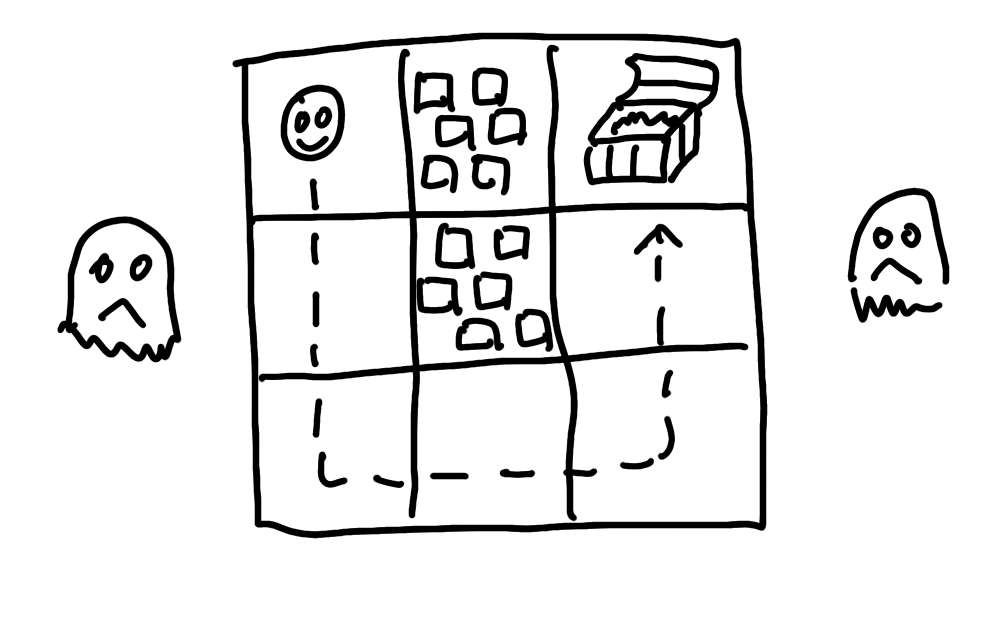
\includegraphics[width=4cm]{images/maze}	
\end{center}

Следите функции ``придвижват'' играча в лабиринта:

\begin{lstlisting}[basicstyle=\small,language=Haskell]
left (Game (x, y) w) = Game (x-1, y) w
right (Game (x, y) w) = Game (x+1, y) w
up (Game (x, y) w) = Game (x, y-1) w
down (Game (x, y) w) = Game (x, y+1) w	
\end{lstlisting}

И помощни функции при изследване на играта:

\begin{lstlisting}[basicstyle=\small,language=Haskell]
foundGold  :: Game -> Bool
foundGold  (Game (x,y) w) = (w !! y) !! x == Gold
stuck  :: Game -> Bool
stuck  (Game (x,y) w) = dead w (x, y)
dead :: [[Tile]] -> Pos -> Bool
dead w (x, y) = x < 0 || x >= length w ||
                y < 0 || y >= length w || 
                (w !! y) !! x == Wall
move :: Game -> (Pos -> Pos) -> Maybe Game
move (Game p w) mv = if dead w (mv p) 
                       then Nothing 
                       else Just $ Game (mv p) w
\end{lstlisting}

\end{mdframed}

\begin{enumerate}[resume]
	\item С помощта на \code{map}, \code{mapMaybe}, \code{filter} и \code{fold} да се намерят:
	\begin{enumerate}[label=\alph*)]
		\item Броя на препятсвията в даден лабиринт
		\item Броя съседи на целта, които не са препятсвия
		\item Дали целта е оградена изцяло от препятствия (\code{True} или \code{False})
	\end{enumerate}

	\item(*) С помощта на \code{foldr} да се дефинира функция, която проверява дали дали даден списък от числа \code{l::[Int]} е нареден във възходящ ред. \emph{Упътване: Използвайте двойка \code{(Bool,Int)} за акумулатор.}

\end{enumerate}

\section {$\lambda$ функции}

\begin{enumerate}[resume]
	\item Да се дефинира функция \code{caseof :: [a->Bool] -> [a->b] -> a->b}. Функцията приема $k$ на брой предиката над $a$ и $k$ на брой функции $a\rightarrow b$. Функцията \code{caseof} връща функция, която приема елемент $x$ от тип $a$ и връща резултата от първата функция, за която предикатът е изпълнен за $x$. Ако няма такава функция, функцията връща резултата от последната функция в списъка. Например, функцията:
\begin{lstlisting}[basicstyle=\small,language=Haskell]
myf = caseof [even, odd] [(\x -> x+1), (\x -> x-1)]
\end{lstlisting}
	ще увеличава с единица четните числа и ще намалява с единица нечетните числа.
		
	\item   Да се дефинира функция \code{createfn :: [(a,b)]->a->b}, която по даден списък от двойки $(a_i,b_i)$, връща функция $f:a \rightarrow b$ дефинирана за всички $a_i$, така че $f(a_i)=b_i$. Например:

\begin{lstlisting}[basicstyle=\small,language=Haskell]
createfn [(1,2),(2,4),(3,6)] 2 -> 4
\end{lstlisting}

\item Да се дефинира функция \code{integrate :: (Double->Double) -> Int -> Double -> Double -> Double}, която по функция $f: Double \rightarrow Double$ и цяло положително число $N$ връща $i(a,b)$ от тип $i:Double \times Double \rightarrow Double$, изчисляваща приближено стойността на определния интеграл $\int_{a}^{b} f(x) dx$ (приемайки, че такъв съществува) по метода на трапеците, по-специално Chained trapezoidal rule\cite{trapezoidal} с $N$ на брой подинтервала. (вж. фиг. \ref{fig:trapezoidal})

\section {Вход/Изход}


\begin{mdframed}[hidealllines=true,backgroundcolor=gray!20]
\textbf{Пренасочване на стандартния вход и изход}

Когато една програма се изпълнява от операционната система, тя получава достъп за четене до поток от данни, неречен ``стандартен вход'' и достъп за писане до ``стандартен изход''. Ако програмата е стартирана в терминална сесия под Posix операционни системи (Mac OS, Linux) или Windows, стадртният вход се състои от поредицата символи, въведени от потребителя чрез клавиатурата. Стандртният изход се визуализира под формата на символи на терминалния прозорец. Това позволява така наречените ``конзолни проложения'', които са предвидени да работят в терминал, да реализират диалогов интерфейс с потребителя. На езика C++, стандартния вход и изход са достъпни чрез потоците \code{cin} и \code{cout}, дефинирани в \code{iostream}. На езика Haskell, достъп до стандартният вход и изход се осъществява чрез функции като \code{getLine}, \code{putStr} и \code{putStrLn}.

Операционните системи позволяват стандартния вход да бъде пренасочен така, че вместо от въведените чрез клавиатурата символи, входът да се състои от съдържанието на файл или от изхода на друга програма. Стандартният изход може да бъде пренасочен така, че вместо да се визуализира на терминала, да се запише във файл или да бъде предаден като вход на друга програма.

При Posix операционните системи, пренасочването на входа от файл или изхода към файл става така: 
\begin{lstlisting}[basicstyle=\small,language=bash]
./myprog < input.txt
./myprog > output.txt
\end{lstlisting}

Съответно, пренасочването на изхода на една програма като вход на друга става така:
\begin{lstlisting}[basicstyle=\small,language=bash]
ls -l | ./myprog
\end{lstlisting}
При тази команда, изходът на командата \code{ls} се подава като вход на програмата \code{myprog}.

Под Windows, пренасочването на входа и изхода от файл става по аналогичен начин:
\begin{lstlisting}[basicstyle=\small,language=bash]
myprog.exe < input.txt
myprog.exe > output.txt
\end{lstlisting}
\end{mdframed}

\item Да се деифнира програма, която прочита изхода на командата \code{ls -l} под MacOS и Linux или \code{dir} под Window и извежда на стадартния изход:
\begin{enumerate}[label=\alph*)]
	\item Броят на файловете и броят на поддиректориите в текущата директория
	\item Броят на файловете в текущата директория с разширение \code{.hs}
	\item Името на най-големия файл в текущата директория
	\item Името на най-новия файл в текущата директория
\end{enumerate}

\begin{mdframed}[hidealllines=true,backgroundcolor=gray!20]
\textbf{Форматът CSV}


Форматът ``Comma Separated Values (CSV)'' е текстов формат за представяне на таблични данни. В CSV формат, всеки ред от таблицата се представя като поредица от стойности, разделени със запетаи. 

Например:
\begin{verbatim}
Kalin Georgiev,M,01-01-1981
Maria Ivanova,F,05-05-2003
\end{verbatim}

Ако в рамките на дадена стойност се съдържа символът за запетая, за да не се интерпретира той като разделител, цялата стойност се поставя в двойни кавички. От друга страна, ако искаме самият низ да съдържа двойни кавички, то всяка дойна кавичка в него ограждаме с други две. Например следния низ:
\begin{verbatim}
"Hello """world""", have a nice day!"
\end{verbatim}
се интерпретира като стойността \verb#Hello "world", have a nice day!#.

\end{mdframed}

\item Да се дефинира функция \code{parseCSV :: String -> [[String]]}, която по даден ред от \code{csv} файл, представен като символен низ, връща списък от символни низове, представляващи стойностите му, като се разглеждат случаите на стойности, оградени с двойни кавички.

Разгледаната в задача \ref{zad:split} функция \code{split} разеделя символния низ спрямо даден разделител, в случая запетая. Резултатът от функцията може да се обработи допълнително:
\begin{enumerate}[label=\alph*)]
	\item Да се слее в един низ всяка редица от съседни елементи $a_i,a_{i+1},...,a_k$, такава че (1)$a_i$ започва с двойна кавичка;  (2)$a_k$ завършва с двойна кавичка; (3)никой от останалите $a_{i+1},...,a_{k-1}$ не започва или завършва с двойна кавичка. \emph{Упражнете се да ивършите тази трансформация чрез }\code{fold}.
	\item се заместят всички срещания на три последователни двойни кавички \verb#"""# с една двойна кавичка \verb#"#.
	\item Функцията да се преработи до \code{Maybe [[String]]} и да разглежда случаи на грешна употреба на кавички -- например две последователни кавички. Кои са всички възможни случаи на грешна употреба на кавички?
\end{enumerate}

\end{enumerate}


\section {Индуктивни типове данни}


\begin{mdframed}[hidealllines=true,backgroundcolor=gray!20]
\textbf{Gantt диаграми}

В управлнието на проекти, \href{https://en.wikipedia.org/wiki/Gantt_chart}{Gantt диаграмите} предоставят начин за визуализане на задачите, от които се състои даден проект, както и за анализ на зависимостите между тях. В тези диаграми всяка задача се характеризира с начало и продължителност. Някои от елемените на диграмата са ``обобщени задачи'', т.е. задачи, коието се сътоят от други задачи, както прости, така и обобщени.
\end{mdframed}

\begin{mdframed}[hidealllines=true,backgroundcolor=gray!20]
\textbf{Работа с дати в Haskell}

Модулът \href{https://hackage.haskell.org/package/time-1.14/docs/Data-Time-Calendar.html}{Data.Time.Calendar} дава удобни стредства за работа с дати от грегорианския календар. Основният тип \code{Day} представя конкретна дата от календара. Функции като \code{addDays} и \code{diffDays}, както и операторите за сравнение, дават възможност за изчисления с дати и сравнения на дати. Чрез \code{read} може да се иницилизира дата от символен низ във формат "YYYY-MM-DD". Функцията \code{show} позволява преобразуване на дата към символен низ.


Например, ако \code{start} е дадена дата в миналото, a \code{today} е текущата дата, то изразът \code{(addDays n start) > today} е истина, ако задача, която е започнала на дата \code{start} и е с продължителност n дни, е приключила към днешна дата.

\end{mdframed}

\begin{enumerate}[resume]
	\item Да се дефинира индуктивен тип \code{Task}, който представя задача от Gantt диаграма. Задачата може да бъде или проста (\code{SimpleTask}), или обобщена (\code{ComplexTask}). Простите задачи се характеризират с име, начало и продължителност. Обобщените задачи се характеризират с име и списък от подзадачи, които могат да бъдат както прости, така и обобщени. 
	
	Да се дефинира функция \code{completed :: Task -> Day -> Bool}, която по задача и дата връща дали задачата е приключила към тази дата. 

	\item Да се дефинира функция \code{duration :: Task -> Int}, която по задача връща нейната продължителност в дни. Продължителността на обобщена задача представлява разликата между дата на започване на най-рано започващата ѝ подзадачи и дата на приключване на най-късно приключващата ѝ подзадача. 
	
	\item \label{zad:tasksxml} Да се реализира извеждане на информацията за задача във \code{xml}-подобен формат. Например:
\begin{lstlisting}[basicstyle=\tiny,language=xml]
<complex descr="Take a course">
	<complex descr="Study">
		<simple descr="Read Textbook" start="2025-02-01" duration="20"/>
		<simple descr="Do homeworks" start="2025-02-10" duration="20"/>
	</complex>
	<simple descr="Take Exam" start="2025-03-01" duration="1"/>
</complex>
\end{lstlisting}

	\item(*)При извеждането на информацията за задача във \code{xml}-подобен формат, да се извърши индентация на вложените елементи, както е в примера на задача \ref{zad:tasksxml}.
	

\end{enumerate}


\pagebreak


\begin{thebibliography}{99}

\bibitem{sbornik}	Магдалина Тодорова, Петър Армянов, Дафина Петкова, Калин Георгиев, ``Сборник от задачи по програмиране на C++. Първа част. Увод в програмирането''
\bibitem{tprog} А. Дичев, И. Сосков, ``Теория на програмите'', Издателство на СУ, София, 1998
\bibitem{pusheen} Wikihow, How to Draw Pusheen the Cat, https://www.wikihow.com/Draw-Pusheen-the-Cat
\bibitem{floyd} R. W. Floyd. ``Assigning meanings to programs.'' Proceedings of the American Mathematical Society, Symposia on Applied Mathematics. Vol. 19, pp. 19–31. 1967.
\bibitem{tpsbornik}	Александра Соскова, Стела Николова, ``Теория на програмите в задачи'', Софтех, 2003
\bibitem{cindy}	David Matuszek, ``Backtracking'', https://www.cis.upenn.edu/~matuszek/cit594-2012/Pages/backtracking.html.
\bibitem{sbornik2} Магдалина Тодорова, Петър Армянов, Дафина Петкова, Калин Николов, ``Сборник от задачи по програмиране на C++. Втора част. Обектно ориентирано програмиране''
\bibitem{trapezoidal} Trapezoidal rule, https://en.wikipedia.org/wiki/Trapezoidal\_rule


\end{thebibliography}

\end{document}
